\documentclass[11pt]{article}
\usepackage[english]{babel}
\usepackage{amsmath,amssymb,amstext}
\numberwithin{equation}{section}
\usepackage{graphicx}
\usepackage{parskip}
\usepackage{float}
\usepackage{tabularx}
\usepackage{amsmath}
\numberwithin{figure}{section}
\numberwithin{table}{section}
\usepackage{placeins}
\usepackage{esint}
%\usepackage{subtextbf}
\usepackage{pdfpages}
\usepackage{url}
%\usepackage{cite}
\usepackage{array}
\usepackage{multirow}
\usepackage[
colorlinks=true,
linkcolor=black,
citecolor=black,
urlcolor=black
]{hyperref}
\usepackage[style=numeric, backend=bibtex]{biblatex}
\usepackage{todonotes}
\usepackage{subcaption}
\usepackage{multirow}
\usepackage{upgreek}
\usepackage{circuitikz}
\usepackage[labelfont=bf,labelsep=space]{caption}
\DeclareCaptionLabelSeparator{tab}{\hspace{1em}} % adjust 1em as needed
\captionsetup[figure]{labelfont=bf,labelsep=tab}

\usepackage{cleveref}
\crefname{equation}{Equation}{Equations}
\Crefname{equation}{Equation}{Equations}





\addbibresource{references/references.bib}
\setlength{\textwidth}{15 true cm}
\setlength{\textheight}{22 true cm}
\oddsidemargin  0.5 cm
\evensidemargin 0.5 cm
\topmargin      0 cm

\renewcommand{\textfraction}{.2}
\renewcommand{\floatpagefraction}{.8}

\begin{document}
%\frontmatter
\pagenumbering{roman}

% Include titlepage
\begin{titlepage}	
	{\sffamily		
		\begin{center}			
			\includegraphics[width=30mm]{content/img/TU_Graz_Logo.png}
			
			\vfill\vfill\vfill
			\vfill\vfill\vfill
			
			{Simon Prato}
			% Author with existing titles
			
			\vfill\vfill\vfill
			
			{\LARGE\bfseries{Numerical Investigation of TEM Cells and Antenna Coupling}}
			% Title of the thesis			
			
			\vfill\vfill\vfill
			\vfill\vfill\vfill			
			
			{\bfseries\large{Master Thesis}}
			
			{Studies: {Electrical Engineering}}
						
			\vfill\vfill\vfill			
			
			submitted to
			
			\vfill
			
			{\bfseries\large{Technical University of Graz}}			
			
			\vfill\vfill\vfill			
			
			Supervisor
			
			{Dr. Thomas Bauernfeind}
			
			\vfill
			
			\vfill
			
			\includegraphics[width=30mm]{content/img/igte_logo.png}
			
			%% OPTIONAL: second supervisor/name of the faculty, etc.
					
			\vfill\vfill\vfill
					
			{Graz}, {August}~{2024}
			
		\end{center}
	}%% end sffamily
\end{titlepage}

\newpage

% Kurzfassung
\iftrue
\cleardoublepage
\setcounter{page}{2}
\vspace*{2.2 cm}
{\Large
\noindent
{\bf Abstract}} \\
\vspace*{0.3 cm}

\noindent

% Abstract
\cleardoublepage
\fi

\selectlanguage{english}
%\listoftodos
% Inhaltsverzeichnis
	\tableofcontents  

% Tabellenverzeichnis
% optional
\newpage
	\listoffigures 

% Abbildungsverzeichnis
% optinal
\newpage
	\listoftables
	
\cleardoublepage

%\mainmatter
\pagestyle{headings}
\pagenumbering{arabic}

\section{Introduction}
% !TeX root = Documentation.tex

In recent years, electronic systems have demonstrated a clear trend toward reduced physical dimensions and increased operating speeds, consequently, higher frequencies are used. As a result, these systems often contain small conducting structures that carry currents and voltages with high amplitudes and frequencies. These structures tend to radiate and are susceptible to electromagnetic radiation, behaving as antennas and causing electromagnetic compatibility (EMC) issues.

Taking EMC into account during the design of electronic systems helps to minimize additional costs and schedule delays that may arise from potential redesigns. Furthermore, it ensures that the product operates reliably when exposed to interference from external sources \cite[p.~64]{Paul_Scully_Steffka_2023}. Consequently, research focusing on all aspects of EMC is conducted regularly. This thesis aims to contribute to these ongoing investigations, specifically through analysis of the previously mentioned small antennas and their coupling behavior in TEM cells. TEM cells are included because they provide a standardized method for measuring electromagnetic emissions under approximate free-space conditions and have been widely used for testing small devices \cites{9153508,Koepke_1989,809846}.

Several studies have analyzed the coupling behavior of small antennas and devices with TEM cells \cites{Sreenivasiah_Chang_Ma_1981, 10274360}. Specifically, \cites{Kreindl_Bauernfeind_Weiss_Stockreiter_Kaltenbacher_2024, 10742020, Wilson_1981} implement electric and/or magnetic dipole moments to model the radiated fields of such antennas, which provide information about the electric and magnetic coupling with the TEM cell, respectively. The magnitudes of the dipole moments are found by measurements with the TEM cell \cite{Sreenivasiah_Chang_Ma_1981} or numerical analysis \cite{10742020}. This thesis treats the coupling behavior of small antennas modeled with dipole moments using the latter approach, namely numerical computation using the finite element method. The advantage of this approach is the absence of inaccuracies caused by the measurement setup or related uncertainties, allowing the analysis to focus on the underlying mechanics behind the coupling behavior.

This thesis aims to explain how the electric and magnetic dipole moments of antennas are created and what factors affect them. Understanding this helps design electronic devices that meet EMC requirements and achieve specific coupling behaviors. Additionally, replacing the small antennas with their equivalent dipole moments significantly reduces computational effort, which is particularly advantageous when dealing with large computational domains.

Furthermore, this thesis investigates the shielding efficiency of different materials in the presence of dipole moments. The performance of the shielding material with respect to the electric and magnetic coupling behavior of the antennas, as reflected by the dipole moments, is investigated. The results assist in the selection of appropriate shielding material to effectively reduce emissions produced by the antennas. 

To achieve these objectives, this thesis first presents the theoretical foundations of electric and magnetic dipole moments in \cref{sec:dipole-theory}. The behavior of electromagnetic waves generated by arbitrary sources in waveguides, specifically the TEM cell, is then discussed in \cref{sec:guided-waves}. Further, background information of electromagnetic shielding and methods to determine shielding effectiveness using the TEM cell are presented. A brief overview of the finite element method is provided in \cref{sec:simulations}. 

Subsequently, \cref{sec:num-inv} addresses the numerical modeling of antennas and the TEM cell and investigates the generation of electric and magnetic dipole moments for monopole and loop antennas using the theoretical framework developed earlier. This knowledge is applied to three additional antennas, whose analysis delivers results closely related to that of the monopole and loop antennas due to their shared predominantly inductive or capacitive characteristics, which emerge as the primary distinction in the antenna coupling behavior. Equivalent circuits to model capacitive and inductive antennas, together with the TEM cell and their coupling paths, are developed, from which the dipole moments can be investigated in more detail.

\cref{sec:shielding-sim} demonstrates the application of shielding materials in numerical simulations involving dipole moments and electrically small antennas. Lastly, \autoref{sec:conclusions} presents the conclusions and discussion derived from this thesis, along with potential directions for future research.



\section{Dipole Theory}

Magnetic and electric dipoles are an effective approach for modeling the radiation of electrically small antennas. They are defined as antennas with dimensions much less than one-tenth of the wavelength ($l\ll\lambda$)\cite[p. 151]{Balanis_1997}. By calculating the respective dipole moments, the coupling between antennas and TEM cells can be numerically estimated. This section provides a brief introduction to the underlying theory of this concept.

\subsection{Electric Dipoles}

An electric dipole is described as two tiny charged metal spheres or two capacitor-plates, which are connected with a linear wire of length $d$ and diameter $a$ \cite[p. 467]{Griffiths_2024}, \cite[p. 151]{Balanis_1997}. The charges move and accelerate along the wire, creating radiation. In case of an ideal, infinitesimal dipole, the wire is very thin ($a\ll \lambda$) and very small ($d \ll \lambda$) compared to the wavelength $\lambda$ \cite[p. 151]{Balanis_1997}, \cite[p. 468]{Griffiths_2024}. For an antenna to be accurately modeled as an infinitesimal electric dipole, its length usually must be smaller than a fiftieth of the wavelength ($d < \lambda/50$) \cite[p. 156]{Balanis_1997}. They are not very practical, but serve as a basic building block for more complex geometries. The current is spatially uniform throughout the wire.

Wires that are too long to be modeled as an infinitesimal dipole, but short enough to be considered electrically small ($\lambda / 50 < l \leq \lambda/10$), are classified as short physical dipoles \cite[pp. 162-163]{Balanis_1997}. They are a more accurate and useful representation of a linear wire antenna, and investigated further. In the remainder of this thesis, the term electric dipole refers specifically to short physical electric dipoles. Furthermore, time variation according to $\mathrm{e}^{-j\omega t}$ is assumed and therefore omitted.

A current $I_0$ is fed into the short, center-fed, linear antenna shown in \autoref{fig:electric_dipole}. The current along the antenna arms $I(z)$ linearly drops to zero \cite[p. 412]{Jackson}, as visualized in \autoref{fig:electricdipolecurrent}. Mathematically, it is described by, 

\begin{equation}
    I(z)= I_0\left( 1-\frac{2|z|}{d} \right).
    \label{eqn:current_dipole}
\end{equation}


\begin{figure}[h]
    \centering
    \includegraphics[width=0.5\linewidth]{content/10_theory/img/electric_dipole_drawing.png}
    \caption{Geometrical arrangement of a linear center-fed wire antenna.}
    \label{fig:electric_dipole}
\end{figure}

Charge accumulates along the antenna's arms. It is expressed as a charge per unit length $\rho'$ due to the thin wire. It is derived by the continuity equation,

\begin{equation}
    \rho' = \pm\frac{\mathrm{d}}{\mathrm{d}z}j\frac{ I(z)}{\omega} = \pm j\frac{2  I_0}{\omega d}.
    \label{eqn:charge_distribution_dipole}
\end{equation}

$\rho'$ is uniformly distributed along each antenna arm \cite[p. 412]{Jackson}.




An important metric is the electric dipole moment $\mathbf{p}$. It is defined as the product of charge density $\rho$ along the antenna and their source point $\mathbf{x'}$ \cite[p.410]{Jackson}, and generally expressed as 

\begin{equation}
	\mathbf{p} = \iiint_V\mathbf{x'} \rho (\mathbf{x'})\mathrm{d}\mathbf{x'}.
	\label{eqn:elec_dipole_mom}
\end{equation}

The vector $\mathbf{x}=\mathbf{\hat{a}}_x x + \mathbf{\hat{a}}_y y + \mathbf{\hat{a}}_z z$ represents the observation point coordinates, while $\mathbf{x'}=\mathbf{\hat{a}}_x x' + \mathbf{\hat{a}}_y y' + \mathbf{\hat{a}}_z z'$ represents the source point coordinates. The vectors $\mathbf{\hat{a}}_x$, $\mathbf{\hat{a}}_y$, and $\mathbf{\hat{a}}_z$ are unit vectors along the x-, y-, and z-directions, respectively. The integration is performed over the volume $V$ of the antenna.

Knowing the charge distribution $\rho'$ enables the calculation of the electric dipole moment $\mathbf{p}$ through \autoref{eqn:elec_dipole_mom}. This results in, 

\begin{equation}
    \mathbf{p}=\int_{-\frac{d}{2}}^{\frac{d}{2}}z\rho'(z)\,\mathrm{d}z\cdot\mathbf{\hat{a}}_z = j\frac{I_0d}{2\omega}\cdot\mathbf{\hat{a}}_z.
    \label{eqn:dipole_mom_example}
\end{equation}

The electric dipole moment $\mathbf{p}$ is parallel to the antenna's arms and points in the z-direction \cite[p. 412]{Jackson}, \cite[p. 155]{Griffiths_2024}. Next, the vector potential $\mathbf{A}$ is determined. It is generally defined as  \cites[p. 152]{Balanis_1997}[p. 410]{Jackson},
 
\begin{equation}
    \mathbf{A}(\mathbf{x})=\frac{\mu}{4\pi}\frac{\mathrm{e}^{-jkr}}{r}\iiint_V \mathbf{J}(\mathbf{x'})\mathrm{d}\mathbf{x'}.
    \label{eqn:vector_pot}
\end{equation}


The variable $r$ is the distance from any source point to the observation point $\left| \mathbf{x}-\mathbf{x'} \right|$. The permeability is described by $\mu$ and the term $\mathrm{e}^{jkr}$ the propagation of the wave, where $k=2\pi/\lambda$ is the propagation factor, or often called wavenumber \cite[p. 704]{Balanis_1997}. $\mathbf{J}$ is the current density in the source region. The calculations of $\mathbf{A}$ simplify to \cite[p. 410]{Jackson},

\begin{equation}
    \mathbf{A} (\mathbf{x})=-j\frac{\mathrm{\mu\omega}}{4\pi}\mathbf{p}\frac{\mathrm{e}^{-jkr}}{r}
    \label{eqn:vector_pot_elec_dipole}
\end{equation}
%Should the calculation of fields even be included? I don't need them for research. But the Field equations are important for explaining the frequency behavior of the electric dipole moment. This can be done by the radiation resistance in \autoref{eqn:elec_rad_res}. In our example, the radiation power depends on the frequency squared ($\mathbf{p}$\textasciitilde

\begin{figure}[t]
	\centering
	\includegraphics[width=0.3\linewidth]{content/10_theory/img/electric_dipole_current}
	\caption{Current distribution across linear wire antenna. It has a maximum at the feedpoint, and drops to zero at points $d/2$ and $-d/2$.}
	\label{fig:electricdipolecurrent}
\end{figure}


Any other field quantities can be derived out of the vector potential $\mathbf{A}$, such as the electric field intensity $\mathbf{E}$ and magnetic field intensity $\mathbf{H}$. This is achieved in a simpler way, when first transforming the Cartesian components of $\mathbf{A}$ into spherical ones, as demonstrated by \cite[p. 153]{Balanis_1997},

\begin{equation}
	\begin{bmatrix}
		A_r  \\
		A_\theta \\
		A_\phi
	\end{bmatrix} = 	
	\begin{bmatrix}
	\sin \theta \cos \phi & \sin \theta \sin \phi & \cos \theta\\
	\cos \theta \cos \phi &  \cos \theta \sin \phi & - \sin\theta\\
	- \sin\phi  & \cos\phi  & 0
	\end{bmatrix}
		\begin{bmatrix}
		A_x  \\
		A_y \\
		A_z
	\end{bmatrix}
\end{equation}

$\mathbf{E}$ and $\mathbf{H}$ are then expressed by \cite[p. 153]{Balanis_1997},

\begin{subequations}\label{eqn:elec_and_mag_field_dipole}
    \begin{equation}
    \mathbf{H} =\frac{1}{\mu r} \left[ \frac{\partial}{\partial r} (r A_{\theta}) - \frac{\partial A_{r}}{\partial \theta} \right]  \mathbf{\hat{\mathbf{a}}_\phi},
    \end{equation}\label{eqn:h_dipole}
    
    \begin{equation}
    \mathbf{E}=-j\omega\mathbf{A}-j\frac{1}{\omega\mu\epsilon}\nabla\left(\nabla\cdot\mathbf{A}\right).
    \end{equation}\label{eqn:e_dipole}
    
\end{subequations}

Substituting $\mathbf{A}$ into \autoref{eqn:h_dipole} and \autoref{eqn:e_dipole} reduces them to 

\begin{subequations}
	\begin{equation}
		H_r=H_\theta=0,
	\end{equation}
	\begin{equation}
		H_\phi = j\frac{k I_0 l \sin\theta}{4\pi r}\left[1 + \frac{1}{jkr}\right]\mathrm{e}^{-jkr},
	\end{equation}
\end{subequations}

and,

\begin{subequations}
	\begin{equation}
		E_r = \eta \frac{I_0 l \cos \theta}{2\pi r^2}\left[ 1 + \frac{1}{jkr} \right] \mathrm{e}^{-jkr},
	\end{equation}
	\begin{equation}
		E_\theta = j\eta \frac{kI_0 l \sin \theta }{4\pi r}\left[ 1 + \frac{1}{jkr} - \frac{1}{(kr)^2} \right] \mathrm{e}^{-jkr},
	\end{equation}
	\begin{equation}
		E_\phi = 0.
	\end{equation}
\end{subequations}


The total radiated power of the antenna is obtained by integrating the complex Poynting vector $\mathbf{W}$ over a closed surface surrounding the antenna \cite[p. 154]{Balanis_1997}. The real part of the total radiated power provides information about energy transferred by radiation, while the imaginary part about the antenna's reactive behavior. $\mathbf{W}$ is defined by 

\begin{equation}
	\mathbf{W}=\frac{1}{2}\left(\mathbf{E}\times\mathbf{H}^*\right) .
\end{equation}

The real power transfer is derived through the time-averaged Poynting vector $\mathbf{W}_\mathrm{av}$ \cite[p. 160]{Balanis_1997}, which is calculated by

\begin{equation}
    \mathbf{W}_\mathrm{av} = \frac{1}{2} \, \Re \{ \mathbf{E} \times \mathbf{H}^* \}.
    \label{eqn:time_averaged_poynting}
\end{equation}

By integrating the time-averaged real Poynting vector $ \mathbf{W}_\mathrm{av} $ over a closed surface, the radiated power $P_{\mathrm{rad}}$ is determined. The real part of the power is independent of the integrated surface, opposed to the imaginary part. In case of an electric dipole $P_{\mathrm{rad}}$ is expressed as

\begin{equation}
    P_{\mathrm{rad}} = \frac{\mathrm{c}^2\mathrm{Z_0}\mathrm{k}^4}{12\pi}|\mathbf{p}|^2.
    \label{eqn:elec_rad_res}
\end{equation}

The radiated power increases with the frequency squared, as the antenna becomes more efficient. This relation holds over the whole frequency range, as long as the antenna is electrically small.

The short physical electric dipole described in this section approximate the behavior of electrically short antennas. Special care must be taken of the excitation method and shape, as it influences the behavior \cite[p. 413]{Jackson}. Additionally, any antenna investigated through this method must remain as small as possible compared to the wavelength $\lambda$, to reduce any analytical approximation errors. 

\todo[inline]{Image theory may be added for TEM cell explanations \cite[p. 184]{Balanis}}


\subsection{Magnetic Dipoles}

The magnetic dipole is modeled as a current loop with radius $b$, whose axis is perpendicular to the plane of the loop. Its radiated fields are analogous to those of an electric dipole, with the electric and magnetic fields interchanged \cite[p. ]{Balanis_1997}. \autoref{fig:magnetic_dipole_drawing} shows a magnetic dipole.

\begin{figure}[h]
    \centering
    \includegraphics[width=0.5\linewidth]{content//10_theory//img/magnetic_dipole_drawing.png}
    \caption{Magnetic dipole}
    \label{fig:magnetic_dipole_drawing}
\end{figure}

The magnetic dipole moment is given by \autoref{eqn:mag_dipole_moment}.

\begin{equation}
    \mathbf{m}=\frac{1}{2}\int (\mathbf{x} \times \mathbf{J})\mathrm{d}^3x
    \label{eqn:mag_dipole_moment}
\end{equation}

A magnetic dipole can be represented with a current loop, or a magnetic current along a straight path. \autoref{eqn:magn_current_curr_loop} shows the mathematical relation between these two \cite{Balanis_1997}. 

\begin{equation}
    I_m L = \mathrm{i}S\omega\mu_0 I_0
    \label{eqn:magn_current_curr_loop}
\end{equation}

$I_m$ is the magnetic current with the unit $\mathrm{V}$. The area $S$ of the loop is calculated by $b^2\pi$. $I_0$ is the electric current with the unit $\mathrm{A}$ flowing through the loop, and $\mu_0$ is the permeability of free space.

\todo{Add fields and radiation power formulas, if it is needed later}

\subsubsection{Crossed Dipoles}
% Read Bauernfeind's: Crossed Dipole Antennas

% When placing the magnetic dipole in the center of the upper or lower chamber of the TEM cell, and pointing in y-direction, it will generate a TEM-wave. Same goes for the electric dipole, pointing in z-direction. When combining two of these dipole moments, any excitation with the first order TEM mode is possible. This is the main idea for modeling antennas. The relation of the magnetic and electric fields is assumed to be roughly equal to the free space wave impedance. Also, magnetic dipoles create a difference in output voltage of the two ports, while electric dipoles create a increase of voltage in both ports. The power transmitted is the same. However: How are they modeled in HFSS? 

Crossed dipoles can generate a wide variety of radiation patterns. Supposed two dipoles are placed perpendicular to each other and fed 90° out of phase, an omnidirectional radiation pattern in created \cite{7293591}. If the equivalent dipoles of an EUT represents such two dipoles, any mode which can propagate in the TEM cell will do so, and therefore influence the measurement result. It is therefore not only important to know which dipoles there are representing the EUT, but also what phase and magnitude they have. Meaning that not only the dipoles aligned with the TEM mode alone influence the result. 
\todo{Write}

\todo{Dipoles next to conducting planes (balanis, collin)}

% Also, the reflections of the conducting sheets of the TEM cell might enhance the dipoles' gain, therefore artificially supporting a certain mode even more. This property is often used in antennas, where a perfect electric conductor (PEC) is placed a quarter wavelength away from the antenna, hence enhancing the gain \cite{7293591}. 


\input{content/10_dipoles/12_antennas_to_investigate}
\subsection{Radiated Field}\label{sec:rad_fields}
\subsection{Antenna Terminology}
Is this chapter necessary?
\subsection{Field regions}

The field quantities $\mathbf{E}$ and $\mathbf{H}$ have been derived for an infinitesimal electric dipole in \cref{eqn:e_er,eqn:e_et,eqn:e_ep} and \cref{eqn:e_hr,eqn:e_hpt}. They are valid everywhere except for the source region \cite[p. 156]{Balanis_1997}. Depending on the distance $r$ to the dipole, the behavior of the fields changes. This becomes apparent when investigating $E_\theta$ in \autoref{eqn:e_et}, specifically expressions 1 and 2 in

\begin{equation}
	E_\theta = j\eta \frac{kI_0 d \sin \theta }{4\pi r}\left[ 1 + \underbrace{\frac{1}{jkr}}_{\text{expression 1}} - \underbrace{\frac{1}{(kr)^2}}_{\text{expression 2}} \right] \mathrm{e}^{-jkr}.
	\label{eqn:e_et_2}
\end{equation}

If the distance $r < \lambda/2\pi$ $(kr < 1)$, then expression 2 dominates the value in the brackets. Consequently, the energy stored in this region is mostly imaginary. It is referred to as the near-field region.

At $r = \lambda/2\pi$ $(kr = 1)$, expression 1 and 2 are of equal magnitude. This leads to the energy stored \todo{Continue}

\todo[inline]{In case of a short dipole, the field regions change as shown below.}


The region around an antenna may be divided into three sub-regions:
\begin{itemize}
	\item Reactive near-field region
	\item Radiating near-field or Fresnel region
	\item Far-field or Fraunhofer region
\end{itemize}

They are shown in \autoref{fig:fieldregionsantenna}. These regions are distinguished for most antennas using the wavelength $\lambda$ and the largest dimension of the antenna $D$. The nearest region to the antenna, the reactive near-field region, is a sphere with radius $R_1$, which is calculated with \autoref{eqn:region_r1}. It is characterized by the predominantly reactive fields in it. The next region, the radiating near-field region, is located around the first, within a sphere of radius $R_2$ calculated in \autoref{eqn:region_r2}. In there, the radiating fields dominate and the angular field distribution is dependent on the distance to the antenna. In the largest and last region, the far-field region, the angular field distribution is independent of the distance to the antenna \cite{Balanis_1997}.

\begin{subequations}
	\begin{equation}
		R_1=0.62\sqrt{D^3/\lambda}
		\label{eqn:region_r1}
	\end{equation}
	\begin{equation}
	R_2=2D^2/\lambda
	\label{eqn:region_r2}
	\end{equation}
\end{subequations}

\begin{figure}[h]
	\centering
	\includegraphics[width=0.4\linewidth]{content/img/field_regions_antenna}
	\caption{Field regions of an antenna \cite{Balanis_1997}}
	\label{fig:fieldregionsantenna}
\end{figure}

The electrically short antennas located in the TEM cell interact with it mostly through the reactive near-field region. However, if the TEM cell is large and frequencies are high, the coupling occurs over the radiating near-field. There, the field distributions are different, hence the dipole moments couple differently over frequency to the cell. \todo[inline]{Is this even possible without reaching other modes behavior? And demonstrate the fields over frequency and distance, which changes differently in different regions}.

An infinitesimal dipole is taken as an antenna. The fields are calculated through the auxiliary fields, as described earlier by \autoref{eqn:elec_and_mag_field_dipole}, which leads to \autoref{eqn:inf_dipole_h_field} for the magnetic field strength and \autoref{eqn:inf_dipole_e_field} for the electric field strength. Those equations are valid everywhere, except for the source point \cite{Balanis_1997}.

\begin{subequations}\label{eqn:inf_dipole_h_field}
	\begin{equation}\label{eqn:hr_htheta}
		H_r = H_\theta = 0
	\end{equation}
	\begin{equation}\label{eqn:hphi}
		H_\phi = j \frac{k I_0 l \sin \theta}{4 \pi r}
		\left[ 1 + \frac{1}{j k r} \right] e^{-j k r}
	\end{equation}
\end{subequations}


\begin{subequations}\label{eqn:inf_dipole_e_field}
	\begin{equation}\label{eqn:er}
		E_r = \eta \frac{I_0 l \cos \theta}{2 \pi r^2} 
		\left[ 1 + \frac{1}{jkr} \right] e^{-jkr}
	\end{equation}
	
	\begin{equation}\label{eqn:etheta}
		E_\theta = j \eta \frac{k I_0 l \sin \theta}{4 \pi r} 
		\left[ 1 + \frac{1}{jkr} - \frac{1}{(kr)^2} \right] e^{-jkr}
	\end{equation}

	\begin{equation}\label{eqn:ephi}
		E_\phi = 0
	\end{equation}
\end{subequations}

The distance of $\lambda / 2\pi$, leading to $kr = 1$, is called radian distance, where $r$ is the distance to the antenna and $k$ is the free-space wave number. There, the real and imaginary part for both $H_\phi$ and $E_r$ is equal. Furthermore in $E_\theta$, only the $1/(jkr)$ term contributes to the field, because the other terms cancel each other out. The radian distance essentially marks a point of equal imaginary and stored power \cite{Balanis_1997}.

In distances smaller than the radian distance $kr<1$, the fields are largely reactive and located in a reactive near-field region. There, the field strength decreases with the cube of the distance ($\propto 1/r^3$).  
At distances beyond the radian distance (kr > 1), in the intermediate-field region, the field strength decreases with the square of the distance ($\propto 1/r^2$) \cite{Balanis_1997}. This behavior is visualized in \autoref{fig:energyfieldsregions}.

The wave-number $k$ is dependent on the frequency. Therefore, when placing an infinitesimal dipole into a TEM cell, its coupling behavior depends on the distance and the field regions, that couple. For that reason, the $kr$ number shall be investigated over the whole frequency range for different distances.

\begin{figure}[t]
	\centering
	\includegraphics[width=0.5\linewidth]{content/img/energy_fields_regions}
	\caption{Magnitude of the terms $1/(kr)$ and $1/(kr)^2$ depending on distance $r$ \cite{Balanis_1997}}
	\label{fig:energyfieldsregions}
\end{figure}





\subsection{Radiated Power}
Important for the Lorentz Reciprocity Part.



\section{Guided Waves}
\subsection[Lorentz Reciprocity Theorem]{Lorentz Reciprocity Theorem\protect\footnote{This section follows closely the treatment in: Robert E. Collin, \textit{Field Theory of Guided Waves}, IEEE Press, 2015 and Constantine A. Balanis, \textit{Antenna theory: Analysis and design}, Wiley, 1997.}}\label{sec:lorentz_theorem}


Let two source pairs $\mathbf{J}_1$, $\mathbf{M}_1$ and $\mathbf{J}_2$, $\mathbf{M}_2$ exist in a volume $V$, bounded by the closed surface $S$. The medium in $V$ is linear and isotropic. The source pairs generate fields $\mathbf{E}_1$, $\mathbf{H}_1$ and $\mathbf{E}_2$, $\mathbf{H}_2$, respectively, with the same frequency. The fields and source pairs can then be related with \cites[p.~145]{Balanis_1997}[p. 49]{Collin_2015}

\begin{equation}
	-\nabla \cdot (\mathbf{E}_1\times \mathbf{H}_2-\mathbf{E}_2\times \mathbf{H}_1)=\mathbf{E}_1\cdot \mathbf{J}_2+\mathbf{H}_2\cdot \mathbf{M}_1-\mathbf{E}_2\cdot \mathbf{J}_1-\mathbf{H}_1\cdot \mathbf{M}_2.
	\label{eqn:lorentz_rec_theorem}
\end{equation}

Integrating \autoref{eqn:lorentz_rec_theorem} over $V$, and converting the volume integral to a surface integral with the divergence theorem, leads to \cites[p. 145]{Balanis_1997}[p. 50]{Collin_2015}

\begin{align}
    -\oiint_S &(\mathbf{E}_1\times \mathbf{H}_2-\mathbf{E}_2\times \mathbf{H}_1)\cdot d\mathbf{s}'\nonumber\\&=\iiint_V
\left(\mathbf{E}_1\cdot \mathbf{J}_2+\mathbf{H}_2\cdot \mathbf{M}_1-\mathbf{E}_2\cdot \mathbf{J}_1-\mathbf{H}_1\cdot \mathbf{M}_2\right)\cdot dv'.
    \label{eqn:lorentz_rec_theorem_int}
\end{align}

This integral equation relates the coupling of different source points. Additionally, if one of these sources is set to zero, the respective source point can serve as an observation point. Setting all sources to zero allows investigation of the coupling of modal fields in a waveguide to other modes, as the following example shows. Suppose the volume $V$ does not contain sources $\mathbf{J}_1 = \mathbf{M}_1 = \mathbf{J}_2 = \mathbf{M}_2 = \mathbf{0}$. Then, the source-free Lorentz Reciprocity theorem reduces to the condition that the modes in the waveguide must fulfill \cite[pp. 145-146]{Balanis_1997}: 

\begin{subequations}
	\begin{equation}
		\nabla \cdot (\mathbf{E}_1\times \mathbf{H}_2-\mathbf{E}_2\times \mathbf{H}_1)=0,
	\end{equation}
	\begin{equation}
		\oiint_S (\mathbf{E}_1\times \mathbf{H}_2-\mathbf{E}_2\times \mathbf{H}_1)\cdot d\mathbf{s}'=0.
		\label{eqn:modes_waveguide}
	\end{equation}
\end{subequations}

Another application arises when investigating a volume $V$ confined by a perfectly conducting surface $S$, in which the linear current densities $\mathbf{J}_1$ and $\mathbf{J}_2$ flow. Because $\mathbf{n}\times\mathbf{E}_1=\mathbf{n}\times\mathbf{E}_2=0$ along the surface $S$, the surface integral in \autoref{eqn:lorentz_rec_theorem_int} vanishes, leading to  

\begin{equation}
	\mathbf{E}_1\cdot\mathbf{J}_2=\mathbf{E}_2\cdot\mathbf{J}_1.
\end{equation}

This is the Rayleigh-Carson form of the Lorentz reciprocity theorem \cite[p. 50]{Collin_2015}. It states that the component of $\mathbf{E}_1$ along $\mathbf{J}_2$ is equal to the component of $\mathbf{E}_2$ along $\mathbf{J}_1$, and vice versa \cite[p. 50]{Collin_2015}. 

In summary, the Lorentz Reciprocity theorem is useful for deriving reciprocal aspects of waveguides, finding orthogonal properties of modes, investigating fields generated by currents and dipole moments in waveguides \cite[p. 50]{Collin_2015}, among several other examples. This theorem will be employed often throughout the remainder of this thesis.

\subsection{Green's Function}

\subsubsection{Scalar Green's Function}\label{sec:scal_green}

Green's function describes the response of a linear differential operator $L$ to a point source as an input, which is modeled by delta-function $\delta$. Its general form is 

\begin{equation}
    \mathrm{L}G(\mathbf{x},\mathbf{x'}) = \delta(\mathbf{x}-\mathbf{x'}).
    \label{eqn:general_greens_funct}
\end{equation}

Once \autoref{eqn:general_greens_funct} is solved and the Green's function $G$ of this specific operator is known, it can be used to solve any input function, such as $u(\mathbf{x})$ in 

\begin{equation}
    Lu(\mathbf{x}) = f(\mathbf{x}).
    \label{eqn:examplary_function_with_operator}
\end{equation}

\todo{What is f(x)?}

This is done by a convoluting 

\begin{equation}
    u(\mathbf{x})=\iiint_V G(\mathbf{x},\mathbf{x'})f(\mathbf{x'})\mathrm{d}\mathbf{x'}
    \label{eqn:examplary_function_solved}
\end{equation}

The Green's function can be used to solve equations involving the Nabla operator $\nabla$ in electrostatics. \autoref{eqn:greens_function_scalar_pot_1} and \autoref{eqn:greens_function_scalar_pot_2} demonstrate how the scalar potential $\phi$ can be calculated from point charge distributions in space $\rho$ by using the Green's function of the Nabla operator. There, the Green's function $G(\mathbf{x},\mathbf{x'}) = \frac{1}{4\pi |\mathbf{x}-\mathbf{x'|}}$ represents the potential at position $\mathbf{x}$ created by an unit point charge at point $\mathbf{x'}$.

\begin{subequations}
\begin{equation}
    \nabla \phi = -\frac{\rho}{\epsilon_0}
    \label{eqn:greens_function_scalar_pot_1}
\end{equation}
\begin{equation}
    \phi(\mathbf{x}) = \frac{1}{4\pi\epsilon_0}\iiint_V\frac{\rho(\mathbf{x'})}{|\mathbf{x}-\mathbf{x'}|}\mathrm{d}V'
    \label{eqn:greens_function_scalar_pot_2}
\end{equation}
\end{subequations}

When boundary conditions are present, the Green's Function may be modified to make the boundary condition vanish. The resulting function is called tailored Green's Function. This proves especially useful in the analysis of guided waves. Another possibility is to construct the Green's Function by a series of reflections on boundaries, applying image theory on perfectly conducting surfaces \cite{Collin_2015}.


%This enables an expansion of the fields in a waveguide excited by an internal source. The perfectly conducting surfaces of the waveguides mirror the source infinitely often. Therefore, the Green's function may be represented by a series of these mirror sources. In practice, these calculations are cumbersome, and only the most significant parts of the series are computed \cite{Collin_2015}. %Should I show mathematical calculations?


\subsubsection{Dyadic Green's Function}\label{sec:dyad_green}

The scalar Green's Function demonstrated in \autoref{sec:scal_green} is useful to solve for one-dimensional functions. However, for the analysis of waveguides, the calculation of the three-dimensional vector potential $\mathbf{A}$ as in \autoref{eqn:helmholtz} is necessary.  

\begin{equation}\label{eqn:helmholtz}
	\nabla^2\mathbf{A}+k^2\mathbf{A}=-\upmu \mathbf{J}
\end{equation}


When replacing $\upmu \mathbf{J}$ by an unit vector source, the solution of the differential equation is shown in \autoref{eqn:sol_dyadic_green}. This is a vector Green's Function by definition.

\begin{equation}\label{eqn:sol_dyadic_green}
	(\mathbf{a}_x + \mathbf{a}_y + \mathbf{a}_z) \frac{e^{-j k |\mathbf{r} - \mathbf{r}_0|}}{4\pi |\mathbf{r} - \mathbf{r}_0|}
\end{equation}

The solution of any current distribution $\mathbf{J}$ can be obtained by superposition, analogous to the scalar Green's Function. A prerequisite is that each component of the current vector $\mathbf{J}$ is each associated with one unit vector of the Green's function, i.e. $J_x$ with $\mathbf{a_x}$, $J_y$ with $\mathbf{a_y}$ and $J_z$ with $\mathbf{a_z}$. This is implemented by using a dyadic Green's Function $\mathbf{\hat{G}}$. The dyadic has a mapping function, rather than an operational one. The dyadic Green's Function is defined as the solution of \autoref{eqn:helmholtz_green}.

\begin{equation}\label{eqn:helmholtz_green}
	\nabla^2 \mathbf{\hat G}(\mathbf{r}, \mathbf{r}_0) + k^2 \mathbf{\hat G} = -\mathbf{\hat I} \delta(\mathbf{r} - \mathbf{r}_0)
\end{equation}

Analogous to the scalar Green's Function, multiplying the unit input function by $\mathbf{\hat{I}}$ leads to the same multiplication of the Green's function, as shown in \autoref{eqn:dyadic_final}.

\begin{equation}\label{eqn:dyadic_final}
	\mathbf{\hat G}(\mathbf{r}, \mathbf{r}_0) = \mathbf{\hat I} \frac{e^{-jk|\mathbf{r} - \mathbf{r}_0|}}{4\pi |\mathbf{r} - \mathbf{r}_0|}
\end{equation}

The dyadic Green's Function is commonly applied to calculate field distributions in waveguides. In \cite{Wilson_1981} it is used to derive the fields in a TEM cell caused by a vertical current conducting wire with help of the small-gap approximation.




\subsection{Modes in TEM Cells}\label{sec:modes_tem_cell}
\subsubsection{Power transfer of modes}
% Goal is to describe the modes in a TEM cell, including their cut-off frequencies. \cite{Kreindl_Bauernfeind_Weiss_Stockreitner_Kaltenbacher_2024} shows that these investigations are important. There are also modes propagating perpendicular to the intended propagation direction. Why are no waveguides used? Explain.

% In this paper, a VCSEL with a decoupling capacitor are modeled. It is visible, that the electric coupling dominates at an orientation of 90°. A local minimum is then visible. At 400\,MHz and upwards, inductive coupling becomes dominant, but only at 0° where it couples with the septum. It is possible, that a certain mode can propagate at a certain frequency, which influenced the result in this paper. 


Any electromagnetic field distribution in a waveguide can be represented by an infinite series of normal modes. \autoref{eqn:norm_power} shows that each mode is orthogonal to each other, with $\mathbf{e_n}^\pm$ and $\mathbf{h_n^\pm}$ being the function vectors of the electric and magnetic field in transverse direction \cite{Collin_2015}. A coupling between the modes only occurs due to geometric changes of the waveguide. Additionally, each mode is normalized to $\sqrt{\mathrm{W}}$, shown by \autoref{eqn:unit_power}. Only the transverse fields are investigated in these Equations, because they carry power along the waveguide, opposed to the fields in the propagation direction.

\begin{align}
    \iint \mathbf{e_n^\pm}\times \mathbf{h_m^\pm}\mathrm{d}S\mathbf{n}&=0 \quad\text{if}\quad n\neq m
    \label{eqn:norm_power}\\
    \iint \mathbf{e_n^\pm}\times \mathbf{h_n^\pm}\mathrm{d}S\mathbf{n}&=1
    \label{eqn:unit_power}
\end{align}

The radiated fields can be described by a summation of normal modes, as in \autoref{eqn:modal_superposition1} and \autoref{eqn:modal_superposition2}. The coefficients of these modes are straightforward to calculate, due to Lorentz Reciprocity Theorem, if the waveguide's walls are perfectly conducting. Ideally, any higher order mode than the first TEM mode will be suppressed, and the calculation simplifies to $n=0$. Additionally, it is assumed that the source is electrically small, which makes it possible to represent it with dipoles, further simplifying the equations \cite{Koepke_1989}. 

\begin{align}
    \mathbf{E^\pm}&=\sum_na_n\mathbf{E_n^\pm}    \label{eqn:modal_superposition1}\\
    \mathbf{H^\pm}&=\sum_na_n\mathbf{H_n^\pm}    \label{eqn:modal_superposition2}
\end{align}

Suppose a current source $\mathbf{J_1}$ excites a waveguide (as is the case with the dipoles in the TEM cell). Normally, such a current source would be driven with external fields, but for the sake of the argument, they are ignored. Only $\mathbf{E}$ and $\mathbf{H}$ are considered, which are the fields radiated by $\mathbf{J_1}$. Additionally, $\mathbf{E}_n^\pm$ and $\mathbf{H}_n^\pm$ are the resulting waveguide fields, with the signs indicating the direction of propagation. Take \autoref{eqn:lorentz_rec_theorem_int} and set $\mathbf{J_2}=\mathbf{M_1}=\mathbf{M_2}=0$. Now, only the current source $\mathbf{J_1}$ remains, and the \autoref{eqn:J1_propagating_waves} emerges. % Explain how certain surfaces do not to have be integrated, therefore rendering this equation very useful. Also, the expansion coefficients can be determined. Maybe do this calculation with a rectangular waveguide.

\begin{equation}
    \oiint _S (\mathbf{E_n^\pm}\times \mathbf{H}-\mathbf{E}\times \mathbf{H}_n^\pm)\cdot\mathrm{d}\mathbf{S}=\iiint \mathbf{J_1}\cdot\mathbf{E_n^\pm}\mathrm{d}V
    \label{eqn:J1_propagating_waves}
\end{equation}

\begin{figure}[t]
	\centering
	\includegraphics[width=0.7\linewidth]{content/img/reciprocity_tem_cell}
	\caption{TEM cell with an arbitrary current source $\mathbf{J}$ along the curve $\mathbf{\tau}$. $\mathbf{E}$ and $\mathbf{H}$ are the field intensities induced by the current. $\mathbf{E}^+$ and $\mathbf{E}^-$ are outgoing fields towards both output ports of the TEM cell. $\mathbf{S}$ indicates the surface, and $V$ the volume of the domain in question.}
	\label{fig:reciprocitytemcell}
\end{figure}


In case of the TEM cell, it is desirable that only the TEM mode is propagating, and that the source is represented by a dipole. When the expansions \autoref{eqn:modal_superposition1}, \autoref{eqn:modal_superposition2} and the orthogonal property \autoref{eqn:norm_power} are used, and when considering an electric dipole, the \autoref{eqn:dipole_tem_waves} arises. In this equation, the wave amplitudes $a$ and $b$ are given through the surface integral in the Lorentz Reciprocity theorem, with $a$ being the wave going to the left side, and $b$ to the other. The electric dipole moment $\mathbf{m_e}$ is given by the current $\mathbf{J}$ flowing through the infinitesimal wire. Note that only the electric field of TEM wave propagation is considered. In reality, more modes may propagate, for which the electric field must be replaced by the superposition of normal modes as in \autoref{eqn:modal_superposition1}. %Additionally, to calculate the exact value of the electric field, a series of image sources as a Green's function may be applied.

\begin{equation}
\begin{pmatrix}a \\b\end{pmatrix} = -\frac{1}{2}\mathbf{m_e}\cdot \mathbf{E}^\pm
\label{eqn:dipole_tem_waves}
\end{equation}
\todo{$E_n^\pm$?}

If this arbitrary current distribution forms an infinitesimal loop, the source can be represented by a magnetic dipole moment $\mathbf{m_m}$. It is defined by the product $\mathbf{m_m}=\mathbf{A}\cdot I$, an infinitesimal current loop with area $A$ carrying a current $I$. This leads to \autoref{eqn:mag_dipole_moment_tem}. This formulation assumes, that the magnetic field strength $\mathbf{H}^\pm$ does not change over the loop area, i.e. the loop is electrically small. Otherwise, the magnetic field strength $\mathbf{H}^\pm$ must be considered in the integration \cite{Collin_2015,Sreenivasiah_Chang_Ma_1981}.

\begin{align}
    \begin{pmatrix}a \\b\end{pmatrix} &= -\oint_C \mathbf{E}^\pm \mathrm{d}l \nonumber \\
    &= -\iint_{S_0} \nabla \times \mathbf{E}^\pm \mathrm{d}\mathbf{S}\nonumber\\
    &= \mathrm{i}\omega\mu_0\iint_{S_0} \mathbf{H}^\pm\cdot \mathrm{d}\mathbf{S}\nonumber\\
    &= \mathrm{i}\omega\mu_0\mathbf{m}_m\mathbf{H}^\pm 
    \label{eqn:mag_dipole_moment_tem}
\end{align}


If there are several modes propagating, it is useful to find the coefficients of the modes $a_n$ and $b_n$ in \autoref{eqn:modal_superposition1} and \autoref{eqn:modal_superposition2}. In this case, the orthogonality property in \autoref{eqn:norm_power} is used to derive \autoref{eqn:an} and \autoref{eqn:bn} \cite{Collin_2015}. The wire is described by a curve C, and the tangential vector $\boldsymbol{\tau}$ is used to integrate along this curve.

\begin{subequations}
    \begin{equation}
        2a_n = -\int_C \boldsymbol{\tau}\cdot\mathbf{E}_n^-\mathrm{d}l
        \label{eqn:an}
    \end{equation}
        \begin{equation}
        2b_n = \int_C \boldsymbol{\tau}\cdot\mathbf{E}_n^+\mathrm{d}l
        \label{eqn:bn}
    \end{equation}
\end{subequations}

\subsubsection{Modes in rectangular waveguides}

A TEM cell is used for EMC test specifications. It makes the conduction of TEM waves possible, which resemble planar free-space waves. Additionally, it shields the waves from radiating to the sides, for which it has a clear advantage to a stripline \cite{809846,990711}. A simple rectangular waveguide cannot be used for this application. Assuming that a monochromatic wave travels down the waveguide, the waves will propagate without dampening only at a certain angle of reflection on the perfectly conducting surface. A short mathematical proof can be shown here, using Maxwell's equation. It shows that the electric and magnetic fields in direction of propagation cannot both be zero. 
\begin{align}
    \mathbf{E}&=(E_{0,x}\cdot\mathbf{e_x}+E_{0,y}\cdot\mathbf{e_y}+E_{0,z}\cdot\mathbf{e_z})\mathrm{e}^{\mathrm{i}(\omega t-kz)}\\
    \mathbf{H}&=(H_{0,x}\cdot\mathbf{e_x}+H_{0,y}\cdot\mathbf{e_y}+H_{0,z}\cdot\mathbf{e_z})\mathrm{e}^{\mathrm{i}(\omega t-kz)}\\
    \nabla \times \mathbf{E} &=\begin{pmatrix}\frac{\mathrm{d}}{\mathrm{d}y}E_z-\mathrm{i}kE_y \\\mathrm{i}kE_x-\frac{\mathrm{d}}{\mathrm{d}x}E_z \\\frac{\mathrm{d}}{\mathrm{d}x}E_y-\frac{\mathrm{d}}{\mathrm{d}y}E_x\end{pmatrix}=\begin{pmatrix} -\mathrm{i}\omega B_x\\-\mathrm{i}\omega B_y\\ -\mathrm{i}\omega B_z \end{pmatrix}\\
    \nabla \times \mathbf{B} &=\begin{pmatrix}\frac{\mathrm{d}}{\mathrm{d}y}B_z-\mathrm{i}kB_y \\\mathrm{i}kB_x-\frac{\mathrm{d}}{\mathrm{d}x}B_z \\\frac{\mathrm{d}}{\mathrm{d}x}B_y-\frac{\mathrm{d}}{\mathrm{d}y}B_x\end{pmatrix}=\begin{pmatrix} \frac{\mathrm{i}\omega}{\mu\epsilon} E_x\\\frac{\mathrm{i}\omega}{\mu\epsilon} E_y\\ \frac{\mathrm{i}\omega}{\mu\epsilon} E_z \end{pmatrix}
\end{align}

If $E_z$ and $B_z$, the fields in direction of propagation, were both zero, then the change of the transverse fields would be constantly zero, and because of the boundary conditions, all transverse fields would be zero. \autoref{eqn:rect_waveguide_gauss} shows Gauss' law and \autoref{eqn:rect_waveguide_faraday} Faraday's law if $E_z=B_z=0$, from which the unchanging transverse electric field can be derived. 

\begin{align}
    \frac{\mathrm{d}}{\mathrm{d}x}E_x+\frac{\mathrm{d}}{\mathrm{d}y}E_y&=0\quad\text{Derived out of Gauss' law}\label{eqn:rect_waveguide_gauss}\\
    \frac{\mathrm{d}}{\mathrm{d}y}E_x-\frac{\mathrm{d}}{\mathrm{d}x}E_y&=0\quad\text{Derived out of Faraday's law}\label{eqn:rect_waveguide_faraday}
\end{align}

\subsubsection{TEM Mode in TEM Cells}

A TEM cell solves this problem, by having a gap between the septum and the side walls. Essentially, it can be considered as two rectangular waveguides with apertures on the sides. Those apertures allow perturbations of the electromagnetic fields between them. The boundary conditions of the Laplace equation now changed due to the gaps. The Green's function may be calculated of the new construction, now considering the boundary conditions at the gaps, which must be the same for both waveguides (to prevent discontinuities). In the papers of Tippet, Chang and Wilson, this new Green's function lead to the excitation of TEM modes in both waveguides \cite{Tippet_Chang_Crawford_1976,Wilson_1981}. However, the gap is assumed to be small, electrically ($\xi g \ll 1$) and compared to the septum width ($g/a \ll 1$) \cite{4091747}. The variable $\xi=\sqrt{k_0^2 - \beta ^2}$ is the transverse (in y-direction) propagation constant, and consists of the free-space wave number $k_0$ and longitudinal (in z-direction) propagation constant $\beta$. The variables $g$ and $a$ are geometry variables of the TEM cell annotated in \autoref{fig:verticalantennatemcell}.

\begin{figure}[h]
	\centering
	\includegraphics[width=0.7\linewidth]{content/img/vertical_antenna_tem_cell}
	\caption{TEM cell with vertical antenna inserted}
	\label{fig:verticalantennatemcell}
\end{figure}


To analyze the fields in a TEM cell, the dyadic Green's function discussed in \autoref{sec:dyad_green} proofs itself to be useful. It is assumed, that a vertical, electrically short antenna is inserted in the top center of the TEM cell. This is modeled by a current distribution in y-direction $\mathbf{\hat J}(\mathbf{x}) = \mathbf{a}_y J(\mathbf{x})$ \cite{4091747}. Accordingly, the Green's function reduces to $\mathbf{\hat G}(\mathbf{x, x'}) = \mathbf{a}_y G(\mathbf{x, x'})$. \todo{Check Vector notation. Is correct for Dyadics?} First, the Green's function for a rectangular waveguide $G_O(\mathbf{x,x'})$ is shown in \autoref{eqn:unperturbed_green} \cite{Balanis_1997}. There, $\eta_0$ is the free-space impedance, $M=m\pi / (2a)$, $N=n\pi/b$ and $K_m=(\xi^2-M^2)^{1/2}$. Furthermore,

$\Delta_n = 
\begin{cases}
	\frac{1}{2}, & n = 0 \\
	1,           & n > 0
\end{cases} $ 

and,

$g_{mn}(\mathbf{x}_t, \mathbf{x}_t') = \left( \frac{2}{ab} \right)
\sin M(x + a) \sin M(x' + a)
\cdot \cos Ny \cos Ny'$

are functions implemented in \autoref{eqn:unperturbed_green}. The components $x$, $x'$ and $y$, $y'$ are part of the vectors $\mathbf{x}_t$, $\mathbf{x}'_t$. 

\begin{equation}\label{eqn:unperturbed_green}
	\tilde{G}_0(\mathbf{x}_t, \mathbf{x}_t') =
	\frac{-\mathrm{j} \eta_0}{k_0} \left\{\sum_{m,n=0}^{\infty} \frac{\Delta_n [M^2 + \beta^2]}{M^2 + N^2 - \xi^2} \; g_{mn}(\mathbf{x}_t, \mathbf{x}_t')
	\right\}
\end{equation}


The TEM cells Green's function by adding a unperturbed term to it \cite{4091747}. The derivation of those Green's Functions is demonstrated in \cite{Wilson_1981}, which uses the same methods described in \cite{Balanis_1997}, as mentioned above.

The perturbed term in \autoref{eqn:perturbed_green} describes the influence of the gaps on the field distribution. They are derived by forcing the tangential fields to be continuous across the gaps, then describing this boundary condition mathematically as a perturbing second Green's function. The rest of the boundary conditions on the are zero due to the geometry of the TEM cell. The functions used are,

\begin{equation*}
L(\beta) = \left[
\ln \left( \frac{8a}{\pi g} \right)
- \frac{\pi}{a} \sum_{m \in \{1,3,5,...\}}^{\infty} \left(
\frac{\cot K_m b}{K_m}
+ \frac{2a}{m\pi}
\right)
\right]^{-1}
\end{equation*}

and, 

\begin{equation*}
f(\mathbf{x}_t) = \sum_{m \in \{1,3,5,...\}}^{\infty} M \frac{\cos K_{m} (b - y)}{K_{m} \sin K_{m} b}
\sin Ma \cos Mx J_0(Mg).
\end{equation*}

To receive the final Green's Function, the unperturbed and perturbed term are added together ${G}(\mathbf{x}_t, \mathbf{x}'_t) = {G}_O(\mathbf{x}_t, \mathbf{x}'_t)+{G}_g(\mathbf{x}_t, \mathbf{x}'_t)$. Naturally, the observation point $\mathbf{x}$ can only be on the upper half in the chamber, where the source is also located \cite{4091747}. 


\begin{equation}\label{eqn:perturbed_green}
	\widetilde{G}_g(\mathbf{x}_t, \mathbf{x}'_t) = \frac{ -j \pi k_0 \eta_0}{2 a^2 s^2} L(\beta) f(\mathbf{x}_t) f(\mathbf{x}'_t)
\end{equation}

Because waves propagating in the TEM cell are assumed to travel into infinity, they might have any longitudinal propagation constant $\beta$. They are not limited by boundary conditions in this direction. It therefore proofs useful to apply a Fourier Series over this variable, as done in \autoref{eqn:greens_fourier}. There, the subscript $t$ indicates only the transverse (xy-plane). 
\todo{This explanation is not directly cited but my interpretation. Make sure that this is correct info.}

\begin{subequations}\label{eqn:greens_fourier}
	\begin{equation}
	G_O(\mathbf{x,x'})=\frac{1}{2\pi}\int^\infty_{-\infty} \tilde{G}_0(\mathbf{x_t,x_t'})\mathrm{e}^{j\beta z}\mathrm{d}\beta
	\end{equation}
	\begin{equation}
	G_g(\mathbf{x,x'})=\frac{1}{2\pi}\int^\infty_{-\infty} \tilde{G}_g(\mathbf{x_t,x_t'})\mathrm{e}^{j\beta z}\mathrm{d}\beta
	\end{equation}
\end{subequations}



Now, the antenna impedance is calculated using the generic \autoref{eqn:antenna_imp}. The Green's Function in this represents the electric field excited by an unit strength dipole \cite{4091747}. Scaled by multiplication with the current density  $\mathbf{J}(\mathbf{x})$ and integrated over the length of the wire, results in the total electric field. Next, by multiplying it by the current distribution $\mathbf{J}(\mathbf{x})$ and integrated over the length of the wire again, leads to the apparent power. In the end, dividing this term by the total current consumption squared $I^2$ leads to the impedance.


\begin{equation}\label{eqn:antenna_imp}
	Z = \frac{-1}{I^2} \int_S \int_{S'} \mathbf{J}(\mathbf{x}) \cdot \mathbf{G}(\mathbf{x}, \mathbf{x}') \cdot \mathbf{J}(\mathbf{x}') \, \mathrm{d}s' \, \mathrm{d}s
\end{equation}

When evaluating the real part of the impedance for the case described here, the radiation resistance results from \autoref{eqn:rad_res}. If the inserted antenna is electrically small, as it is in this case, $d$ reduces the influence of other terms. The most dominant term then, $k_0^2$, results in a quadratic relation of the radiation resistance to the frequency. This agrees with the theoretical framework in the discussion about small dipoles in \autoref{sec:dipoles}, as well as with the simulations results in \autoref{sec:simulations}.

\begin{equation}\label{eqn:rad_res}
	R = \frac{ \pi \eta_0 k_0^2 }{ 4 a^2 } \csc^2{ k_0 d } \, L(k_0) H(k_0)
\end{equation}

Here, 
\begin{equation*}
H(\beta) = \sum_{m' \in \{1,3,5,...\}}^{\infty} h_{m'}(\beta) \sum_{m \in \{1,3,5,...\}}^{\infty} h_m(\beta) J_0(r(M^2 + \beta^2)^{1/2})
\end{equation*}

and,

\begin{equation*}
h_m(\beta) = \frac{M \sin Ma J_0(Mg)}{K_m \sin K_m b} \cdot 
\frac{\cos k_0 d - \cos K_m d}{M^2 + \beta^2}.
\end{equation*}

\todo[inline]{Give a short interpretation of each variable. Subdivide the text into subsections}

% To do this, the electric and magnetic field are described by the wave equations in \autoref{eqn:wave_equ_e_field} and \autoref{eqn:wave_equ_h_field} \cite{Collin_2015}. 

% \begin{subequations}
% \begin{equation}
%     \left(\nabla^2-\mu\epsilon\frac{\mathrm{d^2}}{\mathrm{d}t^2}\right)\mathbf{E}(\mathbf{x})=\mu\frac{\mathrm{d}}{\mathrm{d}t}\mathbf{J}+\frac{\nabla\rho}{\epsilon}
%     \label{eqn:wave_equ_e_field}
% \end{equation}

% \begin{equation}
%     \left(\nabla^2-\mu\epsilon\frac{\mathrm{d^2}}{\mathrm{d}t^2}\right)\mathbf{H}(\mathbf{x})=-\nabla\times\mathbf{J}
%     \label{eqn:wave_equ_h_field}
% \end{equation}
% \end{subequations}

% The Green's function must solve these wave equations, therefore it is formulated as \autoref{eqn:greens_function_wave_equ}. The boundary condition for the Green's function is $\frac{\mathrm{d}}{\mathrm{d}\mathbf{n}}\mathbf{G}=0$, which sets the normal derivative at the boundary to zero. ACHTUNG: ICH GLAUBE, DASS DAS NUR IM FALL \cite{Wilson_1981} FUNKTIONIERT, IN WELCHEM NUR DIE Z KOMPONENTEN BEACHTET WERDEN. DIESE ÄNDERN SICH NICHT ÜBER DIE GAP. This boundary condition applies everywhere, meaning to every conducting surface, as well as the gaps between the septum and the walls of the TEM cell. Consequently, any discontinuities in fields are prevented.

% \begin{equation}
%     \left(\nabla^2-\mu\epsilon\frac{\mathrm{d^2}}{\mathrm{d}t^2}\right)\mathbf{G}(\mathbf{x}-\mathbf{x'})=-\delta(\mathbf{x}-\mathbf{x'})
%     \label{eqn:greens_function_wave_equ}
% \end{equation}

% The solution to this given problem has been solved before \cite{Collin_2015}. Here, the TE guide mode expansion in \autoref{eqn:greens_function_rect_waveguide_solved} are included \cite{Wilson_1981}. THIS IS ONLY Z-COMPONENT OF FIELDS! THERE IS NO VECTOR.

% \begin{equation}
%     \mathbf{G}(\mathbf{x}-\mathbf{x'})=\left(\frac{2}{ab}\right)\sum^\infty_{m,n=0}\frac{\Delta_m\Delta_n}{(K^2_{mn}-k^2)}\cos{\left( \frac{m\pi}{2a}(x+a) \right)}\cos{\left( \frac{m\pi}{2a}(x'+a) \right)}\cos{\left( \frac{n\pi y}{b}\right)}\cos{\left( \frac{n\pi y'}{b}\right)}
%     \label{eqn:greens_function_rect_waveguide_solved}
% \end{equation}

% \begin{itemize}
%     \item $\mathbf{x}$ is the observation point
%     \item $\mathbf{x'}$ is the source point
%     \item $a$ and $b$ are the height and width of the rectangular waveguide
%     \item $m, n$ are the indices of the TE mode
%     \item $x$ is the x-component of the observation point $\mathbf{x}$
%     \item $y$ is the y-component of the observation point $\mathbf{x}$
%     \item $x'$ is the x-component of the source point $\mathbf{x}$
%     \item $y'$ is the y-component of the source point $\mathbf{x}$
%     \item $K_{mn} = \left[ \left( \frac{m\pi}{2a} \right)^2+\left( \frac{n\pi}{b} \right)^2 \right]^{1/2}$
%     \item $k$ is the wave number $\frac{2\pi}{\lambda}$
%     \item $\Delta_m=\begin{cases}1/2, & \text{if } m = 0 \\1,       & \text{if } m \neq 0\end{cases}$ and $\Delta_n=\begin{cases}1/2, & \text{if } n = 0 \\1,       & \text{if } n \neq 0\end{cases}$
% \end{itemize}

% To use the Green's function to solve the magnetic fields, \autoref{eqn:wave_equ_h_field} is multiplied with the Green's function $\mathbf{G}(\mathbf{x}-\mathbf{x'})$, and \autoref{eqn:greens_function_wave_equ} with the magnetic field $\mathbf{H}(\mathbf{x})$. The two resulting equations are subtracted from each other, which leads to \autoref{}.

% \begin{equation}
%     \mathbf{G}(\mathbf{x}-\mathbf{x'})\frac{\mathrm{d^2}}{\mathrm{d}t^2}\mathbf{H}(\mathbf{x})-\mathbf{H}(\mathbf{x})\frac{\mathrm{d^2}}{\mathrm{d}t^2}\mathbf{G}(\mathbf{x}-\mathbf{x'})=-\mathbf{G}(\mathbf{x}-\mathbf{x'})\nabla\times\mathbf{J}(\mathbf{x})+\mathbf{H}(
% \end{equation}

\subsubsection{Higher order modes in TEM cells}

The TEM cell used in the simulation has a width of $a=40\,\mathrm{mm}$ and a height of $b=24\,\mathrm{mm}$. A cross section of the TEM cell with the important dimensions is shown in \autoref{fig:tem_cell_crosssection}. The cutoff frequencies of the higher order TE and TM modes can be approximated by the same formula, shown in \autoref{eqn:cutoff_frequency_rect_waveguide} for rectangular waveguides. However, this is only true, if the septum is very thin ($t/b \ll 0.1$), and for modes with n-even subscripts, i.e. TE\textsubscript{m,2n} and TM\textsubscript{m,2n} modes.

\begin{figure}[h]
    \centering
    \includegraphics[width=0.5\linewidth]{content/img/tem_cell_crosssection.png}
    \caption{Cross section of the TEM cell}
    \label{fig:tem_cell_crosssection}
\end{figure}

\begin{equation}
    f_c = \frac{c}{2} \sqrt{\left(\frac{m}{a}\right)^2 + \left(\frac{n}{b}\right)^2}
    \label{eqn:cutoff_frequency_rect_waveguide}
\end{equation}

\begin{itemize}
  \item \( f_c \): cutoff frequency of the mode \(\text{T}_{mn}\)
  \item \( c \): speed of light in the medium (approximately \(3 \times 10^8 \, \text{m/s}\) in air)
  \item \( a \): wider dimension (broad wall) of the rectangular waveguide (meters)
  \item \( b \): narrower dimension (narrow wall) of the rectangular waveguide (meters)
  \item \( m \): mode index in the \(a\)-direction (integer, \(m \geq 0\))
  \item \( n \): mode index in the \(b\)-direction (integer, \(n \geq 0\))
\end{itemize}

The cutoff frequency of the TE\textsubscript{10} mode is around 3.75\,GHz, according to \autoref{eqn:cutoff_frequency_rect_waveguide}. To verify this, a modal analysis was performed in Ansys HFSS, where an empty TEM cell was modeled with two waveports defined at its output. The resulting S\textsubscript{12}-parameters are presented in\autoref{fig:te01_te10_tem_propagation}. The black line shows the S\textsubscript{12}-parameter over the frequency of the TEM mode, while the blue line demonstrates S\textsubscript{12}-parameter of the TE\textsubscript{10} mode. At a frequency of 3.75\,GHz, the mode propagates without attenuation, where the cutoff frequency $f_\mathrm{c,10}$ is defined. The simulated result comes very close to the analytically determined one. 

The red trace shows a cutoff frequency of $f_\mathrm{c,10}=3.12\,\mathrm{GHz}$ for the TE\textsubscript{01} mode. \autoref{eqn:cutoff_frequency_rect_waveguide} would predict a cutoff frequency of 6.25\,GHz, however, the septum influences n-odd modes like this one. Their cutoff frequencies are shifted to a lower value \cite{Weil_Gruner_1984}. 

The frequency in simulations with the TEM cell will range from 1\,MHz to 3\,GHz. This guarantees that the higher order modes will not influence the simulation results.

%The first TM mode would be the TM\textsubscript{11} mode, since TM\textsubscript{01} and TM\textsubscript{10} do not exist.

In a real TEM cell, a tapered section transform the TEM waveguide to a coaxial transmission line. This section does not cause reflections of waves in TEM mode. However, higher order TE and TM modes get reflected, and because the TEM cell is a high-Q cavity, resonances occur at $\frac{\lambda}{4}$ or $\frac{\lambda}{2}$ \cite{990711}. This is not considered in these simulations, since the simulation model does not contain this tapered section. \todo{Maybe do simulations with such a tapered section. See \cite{990711}}

% \autoref{tab:even_n_modes} shows the cutoff frequencies of the n-even modes. The cutoff frequencies of the n-odd modes either have to be determined by the approximation in \cite{Wilson_Ma_1986} or analyzed numerically. \todo{Do either one of these}


% \begin{table}[h]
%     \centering
%     \begin{tabular}{ccc}
%         Mode & Calculated $f_c$ & Measured $f_c$\\
%         TE\textsubscript{10} & 750\,MHz & \\
%         TE\textsubscript{20} & 1.50\,GHz & \\
%         TE\textsubscript{12} & 3.09\,GHz & \\
%         TM\textsubscript{20} & 1.50\,GHz & \\
%         TM\textsubscript{12} & 3.09\,GHz & \\
%     \end{tabular}
%     \caption{Caption}
%     \label{tab:even_n_modes}
% \end{table}

\begin{figure}[h]
    \centering
    \includegraphics[width=1\linewidth]{content/img/tem_cell_modes.png}
    \caption{Propagation of TEM, TE\textsubscript{01} and TE\textsubscript{10} modes in TEM cell}
    \label{fig:te01_te10_tem_propagation}
\end{figure}




The TEM cell does not only support TEM modes, above their cut-off frequency TE and TM modes begin to propagate. Because the TEM cell is a high-Q cavity, those cut-off frequencies are sharply defined frequencies. Due to imperfections, change in materials or finite conductivity of the conducting plates, wave propagating in the TEM mode may excite higher order TE and TM modes, too \cite{10791592}. A change in material, for example, demands the electric and magnetic field to have a component in the direction of propagation at the discontinuity. A paper by Wilson and Ma present analytical approximations to determine these frequencies \cite{Wilson_Ma_1986}.  There is a long list for the several first few corner frequencies of the first modes. Additionally, a paper by Koch, Groh and Garbe determines the resonance frequencies of the first TE modes analytically \cite{10791592}. The TEM mode is necessarily excited by the geometry of the TEM cell, hence this mode is called essential. The higher order TE and TM modes, which are only excited due to non-uniformity of the TEM cell, are called non-essential modes \cite{990711}.


The first modes propagating after the TEM mode is the TE\textsubscript{10} and TE\textsubscript{01} modes. Their transversal electric fields are depicted in \autoref{fig:transversal_e_fields_tem_cell}. 

\begin{figure}[h]
    \centering
    \begin{subfigure}[b]{0.3\linewidth}
        \centering
        \includegraphics[width=\linewidth]{content/img/tem_cell_mode.png}
        \caption{TEM Mode}
        \label{fig:tem_mode}
    \end{subfigure}
    \begin{subfigure}[b]{0.3\linewidth}
        \centering
        \includegraphics[width=\linewidth]{content/img/te01_mode.png}
        \caption{TE\textsubscript{01}}
        \label{fig:te01_mode}
    \end{subfigure}
    \begin{subfigure}[b]{0.3\linewidth}
        \centering
        \includegraphics[width=\linewidth]{content/img/te10_mode.png}
        \caption{TE\textsubscript{10}}
        \label{fig:te10_mode}
    \end{subfigure}
    \caption{Transversal electric fields in cross section of TEM cell}
    \label{fig:transversal_e_fields_tem_cell}
\end{figure}
\todo{Vector directions are wrong in the pictures. Additionally, update cutoff frequencies.}

The cut-off frequencies are dependent on the dimensions of the TEM cell, as previously shown. \autoref{tab:modes_tem_cell} shows some cut-off frequencies of these modes for different TEM cell dimensions. The TE\textsubscript{10}-mode is independent of the height $b$ of the TEM cell, as would be the case in a rectangular waveguide. Both the TE\textsubscript{10}-mode and the TE\textsubscript{01}-mode are dependent on the width $a$. Note that a port impedance of $50\,\Omega$ is only kept in the case $a=40\,\mathrm{mm}$ and $b=24\,\mathrm{mm}$. This information is important when varying the TEM cell dimension, as is done when investigating near-field ($k\cdot r < 1$) and intermediate-field ($k\cdot r = 1$) coupling. 

\begin{table}[h]
\centering
\caption{Cut-off frequencies of higher order modes depending on TEM cell dimensions}
\label{tab:modes_tem_cell}
\begin{tabular}{|c|c||c|c|}
	\hline
	a [mm]& b [mm]&TE\textsubscript{01} $f_c$ [GHz] &TE\textsubscript{10} $f_c$ [GHz]\\
	\hline\hline
	80 & 24 & 1.89 & 2.05 \\
	\hline\hline
	40 & 24 & 3.17 & 3.76 \\
	\hline\hline
	40 & 48 & 2.10 & 3.76 \\
	\hline
\end{tabular}
\end{table}






\subsection{Radiating Sources in TEM Cells}

\subsubsection{Arbitrary source}

Suppose a current source $\mathbf{J}_1$ excites a waveguide (as is the case with the dipoles in the TEM cell). Normally, such a current source requires external fields to drive it, but for they are neglect for now. Only $\mathbf{E}$ and $\mathbf{H}$ are considered, which are the fields radiated by $\mathbf{J}_1$. $\mathbf{E}$ and $\mathbf{H}$ are solved according to $\nabla \times \mathbf{E}=-j\omega\mu_0\mathbf{H}$ and $\nabla\times\mathbf{H}=j\omega\epsilon_0\mathbf{E}+\mathbf{J}$ \cite[p. 360]{Collin_2015}. Additionally, $\mathbf{e}_n^\pm$ and $\mathbf{h}_n^\pm$ are the resulting waveguide fields, with the signs indicating the direction of propagation. Take \autoref{eqn:lorentz_rec_theorem_int} and set $\mathbf{J}_2=\mathbf{M}_1=\mathbf{M}_2=0$. Now, only the current source $\mathbf{J}_1$ remains, and the \autoref{eqn:J1_propagating_waves} emerges. % Explain how certain surfaces do not to have be integrated, therefore rendering this equation very useful. Also, the expansion coefficients can be determined. Maybe do this calculation with a rectangular waveguide.

\begin{equation}
	\oiint _S (\mathbf{e}_n^\pm\times \mathbf{H}-\mathbf{E}\times \mathbf{h}_n^\pm)\cdot\mathrm{d}\mathbf{s'}=\iiint \mathbf{J_1}\cdot\mathbf{e}_n^\pm\mathrm{d}v'
	\label{eqn:J1_propagating_waves}
\end{equation}

\begin{figure}[htbp]
	\centering
	\includegraphics[width=0.7\linewidth]{content/img/reciprocity_tem_cell}
	\caption{TEM cell with an arbitrary current source $\mathbf{J}_1$ along the curve $\boldsymbol{\tau}$. $\mathbf{E}$ and $\mathbf{H}$ are the field intensities induced by the current. $\mathbf{e}^+_n$ and $\mathbf{e}^-_n$ are outgoing fields towards both output ports of the TEM cell of arbitrary form. $\mathbf{S}$ indicates the surface, and $V$ the volume of the domain in question.}
	\label{fig:reciprocitytemcell}
\end{figure}

\todo[inline]{TODO: Maybe add H fields in figure?}

%In case of the TEM cell, it is desirable that only the TEM mode is propagating, and that the source is represented by a dipole. 

The fields $\mathbf{E}$ and $\mathbf{H}$ radiated by $\mathbf{J}_1$ equal a combination of normals modes. Using the expansions \cref{eqn:a_modal_superposition1,eqn:a_modal_superposition2}, \cref{eqn:b_modal_superposition1,eqn:b_modal_superposition2} lead to

\begin{align}
	\oiint _S (\mathbf{e}_n^+\times \mathbf{H}-&\mathbf{E}\times \mathbf{h}_n^+)\cdot\mathrm{d}\mathbf{s'}=\nonumber\\ \nonumber
	&=\oiint _S (\mathbf{e}_n^+\times \sum_m a_m\mathbf{h}_m^+-\sum_m a_m\mathbf{e}_m^+\times \mathbf{h}_n^+)\cdot\mathrm{d}\mathbf{s'}\\
	&=\sum_m a_m \oiint _S (\mathbf{e}_n^+\times \mathbf{h}_m^+-\mathbf{e}_m^+\times \mathbf{h}_n^+)\cdot\mathrm{d}\mathbf{s'}.
\end{align}

Due to the orthogonal property of \autoref{eqn:norm_power} and the normalization in \autoref{eqn:unit_power}, the coefficients of each mode can be evaluated separately through

\begin{align}
	\oiint _S (\mathbf{e_n^+}\times \mathbf{H}&-\mathbf{E}\times \mathbf{h}_n^+)\cdot\mathrm{d}\mathbf{s'}=\nonumber\\
	&=a_n \oiint _S (\mathbf{e}_n^+\times \mathbf{h}_n^+-\mathbf{e}_n^+\times \mathbf{h}_n^+)\cdot\mathrm{d}\mathbf{s'}=-2a_n.
\end{align}

The coefficient $b_n$ of the fields $\mathbf{e}_n^-$ and $\mathbf{h}_n^-$ are evaluated in the same manner.

In this equation, the wave amplitudes $a_n$ and $b_n$ are given through the surface integral in the Lorentz Reciprocity theorem, with $a_n$ being the wave going to the left side, and $b_n$ to the other. 

One pair of coefficients $a_\mathrm{TEM}$, $b_\mathrm{TEM}$ suffice when investigating the propagation of the TEM mode, only. The fields $\mathbf{e}_\mathrm{TEM}$ and $\mathbf{h}_\mathrm{TEM}$ of the TEM-mode are known \todo{Some plot or table for explanation, plus citation}. Combining them with \autoref{eqn:unit_power} leads to \cite{4091811}

\begin{subequations}
	\begin{equation}
		P_{\mathrm{out1}}=\iint_S \langle \mathbf{S} \rangle \cdot \mathrm{d}\mathbf{s'}= \iint_S \frac{1}{2} \, \Re \{ \left(a\cdot \mathbf{e}_\mathrm{TEM}^\pm\right) \times \left(a\cdot \mathbf{h}_\mathrm{TEM}^\pm\right)^* \}\cdot \mathrm{d}\mathbf{s'} = \frac{|a|^2}{2},
		\label{eqn:power_of_poynting1}
	\end{equation}
	\begin{equation}
		P_{\mathrm{out2}}=\iint_S \langle \mathbf{S} \rangle \cdot \mathrm{d}\mathbf{s'}= \iint_S \frac{1}{2} \, \Re \{ \left(b\cdot \mathbf{e}_\mathrm{TEM}^\pm\right) \times \left(b\cdot \mathbf{h}_\mathrm{TEM}^\pm\right)^* \}\cdot \mathrm{d}\mathbf{s'} = \frac{|b|^2}{2}.
		\label{eqn:power_of_poynting2}
	\end{equation}
\end{subequations}



The Poynting vector $\langle \mathbf{S} \rangle$ of the TEM mode does not have an imaginary component,

\begin{equation}
	\langle \mathbf{S} \rangle=\mathbf{e}_\mathrm{TEM}^\pm\times\mathbf{h}_\mathrm{TEM}^\pm=\Re\{\mathbf{e}_\mathrm{TEM}^\pm\times\left(\mathbf{h}_\mathrm{TEM}^\pm\right)^*\}.
	\label{eqn:equivalent_tem}
\end{equation}



\subsubsection{Equivalent dipole moments}\label{sec:equ-dip-mom}

The electric dipole moment $\mathbf{m_e}$ is given by the current $\mathbf{J}_1$ flowing through the infinitesimal wire.

\begin{equation}
	\begin{pmatrix}a_n \\b_n\end{pmatrix} = -\frac{1}{2}\mathbf{m_e}\cdot \mathbf{e}_n^\pm
	\label{eqn:dipole_tem_waves}
\end{equation}

If this arbitrary current distribution forms an infinitesimal loop, the source can be represented by a magnetic dipole moment $\mathbf{m_m}$. It is defined by the product $\mathbf{m_m}=\mathbf{A}\cdot I$, an infinitesimal current loop with area $A$ carrying a current $I$. This leads to \autoref{eqn:mag_dipole_moment_tem}. This formulation assumes, that the magnetic field strength $\mathbf{h}^\pm$ does not change over the loop area, i.e. the loop is electrically small. Otherwise, the magnetic field strength $\mathbf{h}^\pm$ must be considered in the integration \cite{Collin_2015,Sreenivasiah_Chang_Ma_1981}.

\begin{align}
	\begin{pmatrix}a_n \\b_n\end{pmatrix} &= -\oint_C \mathbf{e}_n^\pm \mathrm{d}l \nonumber \\
	&= -\iint_{S} \nabla \times \mathbf{e}_n^\pm \mathrm{d}\mathbf{s'}\nonumber\\
	&= \mathrm{i}\omega\mu_0\iint_{S} \mathbf{h}_n^\pm\cdot \mathrm{d}\mathbf{s'}\nonumber\\
	&= \mathrm{i}\omega\mu_0\mathbf{m}_m\mathbf{h}_n^\pm 
	\label{eqn:mag_dipole_moment_tem}
\end{align}


If there are several modes propagating, it is useful to find the coefficients of the modes $a_n$ and $b_n$ in \autoref{eqn:modal_superposition1} and \autoref{eqn:modal_superposition2}. In this case, the orthogonality property in \autoref{eqn:norm_power} is used to derive \autoref{eqn:an} and \autoref{eqn:bn} \cite{Collin_2015}. The wire is described by a curve C, and the tangential vector $\boldsymbol{\tau}$ is used to integrate along this curve.

\begin{subequations}
	\begin{equation}
		2a_n = -\int_C \boldsymbol{\tau}\cdot\mathbf{e}_n^-\mathrm{d}l
		\label{eqn:an}
	\end{equation}
	\begin{equation}
		2b_n = \int_C \boldsymbol{\tau}\cdot\mathbf{e}_n^+\mathrm{d}l
		\label{eqn:bn}
	\end{equation}
\end{subequations}

% What is this subsection for? Maybe it should be combined with the TEM cell section. In there, the calculations with Green's theorem and Lorentz Reciprocity Theorem could be put. Then, the calculations from the paper of Sreenivasia could follow. It shows how to find the equivalent Dipole moments. It is important to know which modes are propagating. A Electric dipole, which points in direction of wave propagation, should not influence the result. However, it could create TM modes, which would transfer power to the ports. -> Investigate modes.

An electrically small radiating source may be represented by six dipoles. This number includes three magnetic dipoles pointing in every direction of the Cartesian coordinate system (x, y, and z-direction), and three electric dipoles in the same orientation. Consequently, an equipment under test (EUT) could be modeled with these dipoles, leading to much less computational effort in simulation. The excited EM waves by point sources is discussed in \cite{Collin_2015} and in \autoref{sec:modes_tem_cell}. An analytical procedure to determine these dipole moments is presented by Sreenivasiah \cite{Sreenivasiah_Chang_Ma_1981}, and some experimental results based on it can be found in the research of Kreindl, where bond wires were modeled with magnetic dipoles\cite{Kreindl_Bauernfeind_Weiss_Stockreiter_Kaltenbacher_2024}, and, again, Sreenivasiah \cite{Sreenivasiah_Chang_Ma_1981}.

% Citing: "If the waveguide walls are perfectly conducting, the coefficients of such an expansion may be obtained in a straightforward manner, by an application of Lorentz's reciprocity principle." - This should be treated in the section about TEM cells. A reference to the Lorentz Reciprocity Theorem shall be made, and how it is used to determine the coefficients of the orthonormal modes.

The idea is to place the EUT in the TEM cell and measure the power of both output ports. The amplitudes of the TEM fields are expressed by \autoref{eqn:a_b_moments} \cite{Sreenivasiah_Chang_Ma_1981}.

\begin{equation}
    \begin{pmatrix}a_n \\b_n\end{pmatrix} = \frac{1}{2}(-\mathbf{m_e}\cdot \mathbf{e}_n^\pm+\mathrm{i}\omega\mu_0\mathbf{m_m}\cdot\mathbf{h}_n^\pm)
    \label{eqn:a_b_moments}
\end{equation}

The magnetic field $\mathbf{h}_n$ and electric field $\mathbf{e}_n$ are both normalized to $1\,\sqrt{\mathrm{Hz}}$ \cite{Kreindl_Bauernfeind_Weiss_Stockreiter_Kaltenbacher_2024} and correspond to the TEM mode in free space \cite{Sreenivasiah_Chang_Ma_1981}. The electric dipole moment $\mathbf{m_e}$ and the magnetic dipole moment $\mathbf{m_m}$ are complex vectors, containing an amplitude and phase for every one of the three directions in the coordinate system (x, y, z), and have the units $\mathrm{A\cdot m}$ and $\mathrm{V\cdot m}$. The variables $a$ and $b$ correspond to the amplitudes of the waves in both possible directions in the TEM cell with the unit $\sqrt{\mathrm{W}}$.
This leads to the final form in \autoref{eqn:a_b_moments_simp} \cite{Sreenivasiah_Chang_Ma_1981}.

\begin{equation}
    \begin{pmatrix}a_n \\b_n\end{pmatrix} =-\frac{1}{2}(\mathbf{m_e}\pm jk\mathbf{m_m}\times \mathbf{z})\cdot \mathbf{e}_n^\pm.
    \label{eqn:a_b_moments_simp}
\end{equation}

$\mathbf{m}_{\mathrm{e}}$ and $\mathbf{m}_{\mathrm{e}}$ are separately derived by 

\begin{equation}
	\mathbf{m}_{\mathrm{e}}=\frac{a_n+b_n}{\mathbf{e}_n^\pm},
	\label{eqn:ifa_me}
\end{equation}

\begin{equation}
	\mathbf{m}_{\mathrm{m}}=j\frac{a_n-b_n}{k_0  \mathbf{e}_n^\pm}.	\label{eqn:ifa_mm}
\end{equation}

The unity vector $\mathbf{\hat{a}}_z$ points in direction of propagation. The function vector $\mathbf{e}_n^\pm$ describes the normalized electric field amplitude in traverse direction, i.e. x and y-directions, of the excited fundamental mode. Due to the normalization of the electric and magnetic fields to $1\,\sqrt{\mathrm{W}}$, the total power at one port is 1/2\,W. This defines $\mathbf{e}_n^\pm$ as the electric field of the TEM cell, excited with a peak unit power (1\,W).

The individual components aligned with the x- and y-direction can be investigated separately. For example, the components of $\mathbf{m}_\mathrm{e}$ are derived with

\begin{subequations}
	\begin{equation}
		 m_{\mathrm{ex}} = \frac{2 \sqrt{P_\mathrm{x}}}{e^\pm_{\mathrm{n,x}}},
		\label{eqn:e0x_mse}
	\end{equation}
	\begin{equation}
		m_{\mathrm{\mathrm{ey}}} = \frac{2 \sqrt{P_\mathrm{y}}}{e^\pm_{\mathrm{n,y}}}.
		\label{eqn:e0y_mse}
	\end{equation}
\end{subequations}

$P_\mathrm{x}$ and $P_\mathrm{y}$ describe the power measured at one output port induced by the respective component of the dipole moment \cite{Sreenivasiah_Chang_Ma_1981}. The output power generated by a component of the dipole moment depends on $\mathbf{e}^\pm_{\mathrm{n}}$, therefore on the position in the TEM cell.

In case of the TEM mode, the electric dipole in the TEM cell leads to a increase in power with the same phase in both ports, and a magnetic dipole leads to the same increase, but with a phase shift of $\pm\pi$. This is due to the phase-shift of the magnetic fields at the output ports, as shown in \autoref{fig:reciprocitytemcelltemmode}. 

In case of the next higher-order mode TE\textsubscript{01}, the situation is reversed. An electric dipole moment leads to a phase shift of $\pm\pi$, and a magnetic dipole moment to an absence of a phase shift. This is, again, due to the phase shift between $\mathbf{e}_\mathrm{TE01}^+$ and $\mathbf{e}_\mathrm{TE01}^-$, while there isn't a phase shift present between $\mathbf{h}_\mathrm{TE01}^+$ and $\mathbf{h}_\mathrm{TE01}^-$.

The EUT shall be placed halfway on the septum in $z$-direction to accurately derive electric and magnetic dipole moments. A shift in $z$-direction leads to a phase shift between the powers at the output ports, therefore inducing an error to the results.

It is required to measure the power at the output ports with phase information, which is done with the complex Poynting vector in a numerical analysis. When measuring an EUT with a real TEM cell, the phase information may be found by summing and subtracting the output powers of the ports, as is shown in \cite{Sreenivasiah_Chang_Ma_1981}.

\begin{figure}[htbp]
	\centering
	\includegraphics[width=0.7\linewidth]{content/img/reciprocity_tem_cell_tem_mode}
	\caption{Field distribution of the TEM mode highlighting the out-of-phase magnetic fields at the output ports.}
	\label{fig:reciprocitytemcelltemmode}
\end{figure}


\subsubsection{Electrically small antennas}

The electric field coupling with an electrically small antenna can be simply put as \cite[p. 361]{Collin_2015}

\begin{subequations}
	
	\begin{equation}
		2a_n=-\int_C \boldsymbol{\tau} I(l)\cdot \mathbf{e}_n^+\,dl.
		\label{eqn:e_int_a}
	\end{equation}
	\begin{equation}
		2b_n=-\int_C \boldsymbol{\tau} I(l)\cdot \mathbf{e}_n^-\,dl.
		\label{eqn:e_int_b}
	\end{equation}
	
\end{subequations}

Since the antenna is electrically small, the electric field $\mathbf{e}_n^\pm$ is assumed to be constant in $C$. Furthermore, if the current $I$ is constant along $C$, it does not have to be considered in the integration. Integrating over the closed loop simplifies to \cite[p. 361]{Collin_2015}

\begin{subequations}
	\begin{equation}
		2a_n=-\oint_C \mathbf{e}_n^+\cdot \boldsymbol{\tau}\,dl = j\omega\mu_0 \iint_S \mathbf{h}_n^+\,d\mathbf{s}'=V_n^+,
		\label{eqn:e_a_closed_int}
	\end{equation}
	\begin{equation}
		2b_n=-\oint_C \mathbf{e}_n^-\cdot \boldsymbol{\tau}\,dl = j\omega\mu_0 \iint_S \mathbf{h}_n^-\,d\mathbf{s}'=V_n^-.
		\label{eqn:e_b_closed_int}
	\end{equation}
\end{subequations}

The induced voltage $V_n^+$ causes or is caused by the fields at one port $\mathbf{e}_n^+$, $\mathbf{h}_n^+$, and the induced voltage $V_n^-$ by the fields at the other port $\mathbf{e}_n^-$, $\mathbf{h}_n^-$. The induced voltages $V_n^+$ and $V_n^-$ relate to the magnetic dipole moment $\mathbf{m_m}$ and the coefficients $a$ and $b$. Defining a total induced voltage as $V_n=V_n^--V_n^+$ leads to 

\todo[inline]{Only valid for TEM mode. Make general assumption}

\begin{equation}
	\mathbf{m}_m=\frac{a_n-b_n}{\mathbf{e}_n^\pm\cdot k_0}=\frac{V_n}{\mathbf{e}_n^\pm\cdot k_0}.
	\label{eqn:m_v}
\end{equation}

A magnetic dipole moment $\mathbf{m}_m$ producing fields characterized with coefficients $a_n$ and $b_n$ models the magnetic coupling behavior of any electrically small antenna yielding the same coefficients. Consequently, deriving an equivalent $\mathbf{m}_m$ of an electrically small antenna is possible by measuring $a_n-b_n$ at the output port. 

In a similar manner to \cref{eqn:e_int_a,eqn:e_int_b}, a constant magnetic field $\mathbf{h}_n^\pm$ along $C$, where a magnetic current is present, leads to

\begin{subequations}
	
	\begin{equation}
		2a_n=-\int_C \boldsymbol{\tau} I_m(l)\cdot \mathbf{h}_n^+\,dl,
		\label{eqn:h_int_a}
	\end{equation}
	\begin{equation}
		2b_n=-\int_C \boldsymbol{\tau} I_m(l)\cdot \mathbf{h}_n^-\,dl.
		\label{eqn:h_int_b}
	\end{equation}
	
\end{subequations}

Analogous to \cref{eqn:e_a_closed_int,eqn:e_b_closed_int}, $I_m$ is assumed to be constant and $C$ to form a closed loop, leading to 

\begin{subequations}
	\begin{equation}
		2a_n=-\oint_C \mathbf{h}_n^- \cdot \boldsymbol{\tau}\,dl = -j\omega\epsilon_0 \iint_{S_0} \mathbf{e}_n^+\,d\mathbf{s}',
		\label{eqn:h_a_closed_int}
	\end{equation}
	\begin{equation}
		2b_n=-\oint_C \mathbf{h}_n^+ \cdot \boldsymbol{\tau}\,dl = -j\omega\epsilon_0 \iint_{S_0} \mathbf{e}_n^-\,d\mathbf{s}'.
		\label{eqn:h_b_closed_int}
	\end{equation}
\end{subequations}

Now, further surfaces $S_1$ and $S_2$ are defined. Surface $S_1$ leads, starting from $S_0$, parallel to the electric field $\mathbf{e}_n^\pm$ to infinity. A total surface is defined $S=S_0+S_1+S_2$, where $S_2$ closes the total surface around $S_1$ in infinity\todo{sketch}. Therefore, the total surface covered is closed, and \cref{eqn:h_a_closed_int,eqn:h_b_closed_int} can be written as 


\begin{equation}
	j \omega \epsilon_0 \oiint_{S} \mathbf{e}_n^{\pm} \cdot d\mathbf{s'}=j \omega \epsilon_0 \iint_{S_0} \mathbf{e}_n^{\pm} \cdot d\mathbf{s'}+\underbrace{j \omega \epsilon_0 \iint_{S_1} \mathbf{e}_n^{\pm} \cdot d\mathbf{s'}}_{=0}+\underbrace{j \omega \epsilon_0 \iint_{S_2} \mathbf{e}_n^{\pm} \cdot d\mathbf{S}}_{=0}.
\end{equation}

Inserting Gauss' law $\nabla\cdot \mathbf{E}=\frac{\rho}{\epsilon_0}$ leads to

\begin{equation}
	-j \omega \epsilon_0 \oiint_{S} \mathbf{e}_n^{\pm} \cdot d\mathbf{s'} = -j \omega \epsilon_0 \iiint_{V} \nabla \cdot\mathbf{e}_n^{\pm} \cdot dv' = -j \omega \iiint_{V} {\rho}_n^\pm \cdot dv'.
\end{equation}

With the continuity equation $j\omega\rho = -\nabla\cdot \mathbf{J}$ this leads to

\begin{subequations}
	\begin{equation}
		2a_n = -j \omega \iiint_{V} {\rho}_n^+ \cdot dv' = \iiint_{V} \nabla \cdot \mathbf{J}_n^+ \cdot dv' = \oiint_{S} \mathbf{J}_n^+ \cdot d\mathbf{s'} =I_n^+,
		\label{eqn:charges_a}
	\end{equation}
	\begin{equation}
		2b_n = -j \omega \iiint_{V} {\rho}_n^- \cdot dv' = \iiint_{V} \nabla \cdot \mathbf{J}_n^- \cdot dv' = \oiint_{S} \mathbf{J}_n^- \cdot d\mathbf{s'} = I_n^-.
		\label{eqn:charges_b}
	\end{equation}
\end{subequations}

Relating the obtained expression to the electric dipole moment from \autoref{eqn:ifa_me} with a total current $I_n=I_n^+ + I_n^-$ delivers

\begin{equation}
	\mathbf{m}_e=\frac{a_n+b_n}{\mathbf{e}_n^\pm}=\frac{I_n}{\mathbf{e}_n^\pm}.
	\label{eqn:me_i}
\end{equation}

The physical meaning of $I_n$ is electrical current passing between the septum and the dipole through capacitive coupling with a certain mode, i.e. displacement current. Concluding, the magnetic dipole moment occurs due to induced voltage, while the electric dipole moment due to coupling electric current.

An electric dipole moment $\mathbf{m}_e$ producing fields characterized with coefficients $a_n$ and $b_n$ models the electric coupling behavior of any electrically small antenna yielding the same coefficients. Consequently, deriving an equivalent $\mathbf{m}_e$ of an electrically small antenna is possible by measuring $a_n+b_n$ at the output port. 

Numerical simulations enable the determination of $a+b$ and $a-b$ directly. When applying this described method in a measurement with a real TEM cell, the values are found by adding and subtracting the output powers of both ports, as is shown in \cite{Sreenivasiah_Chang_Ma_1981}.

\subsubsection{Radiation resistance}

\todo[inline]{TODO: Dieses Kapitel eventuell rausnehmen.}

The radiation resistance of an electrically small antenna is derived by applying the Green's function. The following content is mostly taken from \cite{4091747}.

To analyze the fields in a TEM cell, the dyadic Green's function discussed in \autoref{sec:dyad_green} proofs itself to be useful. It is assumed, that a vertical, electrically short antenna is inserted in the top center of the TEM cell. This is modeled by a current distribution in y-direction $\mathbf{\hat J}(\mathbf{x}) = \mathbf{a}_y J(\mathbf{x})$ \cite{4091747}. Accordingly, the Green's function reduces to $\mathbf{\hat G}(\mathbf{x, x'}) = \mathbf{a}_y G(\mathbf{x, x'})$. \todo{Check Vector notation. Is correct for Dyadics?} First, the Green's function for a rectangular waveguide $G_O(\mathbf{x,x'})$ is shown in \autoref{eqn:unperturbed_green} \cite{Balanis_1997}. There, $\eta_0$ is the free-space impedance, $M=m\pi / (2a)$, $N=n\pi/b$ and $K_m=(\xi^2-M^2)^{1/2}$. Furthermore,

$\Delta_n = 
\begin{cases}
	\frac{1}{2}, & n = 0 \\
	1,           & n > 0
\end{cases} $ 

and,

$g_{mn}(\mathbf{x}_t, \mathbf{x}_t') = \left( \frac{2}{ab} \right)
\sin M(x + a) \sin M(x' + a)
\cdot \cos Ny \cos Ny'$

are functions implemented in \autoref{eqn:unperturbed_green}. The components $x$, $x'$ and $y$, $y'$ are part of the vectors $\mathbf{x}_t$, $\mathbf{x}'_t$. 

\begin{equation}\label{eqn:unperturbed_green}
	\tilde{G}_0(\mathbf{x}_t, \mathbf{x}_t') =
	\frac{-\mathrm{j} \eta_0}{k_0} \left\{\sum_{m,n=0}^{\infty} \frac{\Delta_n [M^2 + \beta^2]}{M^2 + N^2 - \xi^2} \; g_{mn}(\mathbf{x}_t, \mathbf{x}_t')
	\right\}
\end{equation}

\begin{figure}[h]
	\centering
	\includegraphics[width=0.7\linewidth]{content/img/vertical_antenna_tem_cell}
	\caption{TEM cell with vertical antenna inserted}
	\label{fig:verticalantennatemcell}
\end{figure}


The TEM cells Green's function by adding a unperturbed term to it \cite{4091747}. The derivation of those Green's Functions is demonstrated in \cite{Wilson_1981}, which uses the same methods described in \cite{Balanis_1997}, as mentioned above.

The perturbed term in \autoref{eqn:perturbed_green} describes the influence of the gaps on the field distribution. They are derived by forcing the tangential fields to be continuous across the gaps, then describing this boundary condition mathematically as a perturbing second Green's function. The rest of the boundary conditions on the are zero due to the geometry of the TEM cell. The functions used are,

\begin{equation*}
	L(\beta) = \left[
	\ln \left( \frac{8a}{\pi g} \right)
	- \frac{\pi}{a} \sum_{m \in \{1,3,5,...\}}^{\infty} \left(
	\frac{\cot K_m b}{K_m}
	+ \frac{2a}{m\pi}
	\right)
	\right]^{-1}
\end{equation*}

and, 

\begin{equation*}
	f(\mathbf{x}_t) = \sum_{m \in \{1,3,5,...\}}^{\infty} M \frac{\cos K_{m} (b - y)}{K_{m} \sin K_{m} b}
	\sin Ma \cos Mx J_0(Mg).
\end{equation*}

To receive the final Green's Function, the unperturbed and perturbed term are added together ${G}(\mathbf{x}_t, \mathbf{x}'_t) = {G}_O(\mathbf{x}_t, \mathbf{x}'_t)+{G}_g(\mathbf{x}_t, \mathbf{x}'_t)$. Naturally, the observation point $\mathbf{x}$ can only be on the upper half in the chamber, where the source is also located \cite{4091747}. 


\begin{equation}\label{eqn:perturbed_green}
	\widetilde{G}_g(\mathbf{x}_t, \mathbf{x}'_t) = \frac{ -j \pi k_0 \eta_0}{2 a^2 s^2} L(\beta) f(\mathbf{x}_t) f(\mathbf{x}'_t)
\end{equation}

Because waves propagating in the TEM cell are assumed to travel into infinity, they might have any longitudinal propagation constant $\beta$. They are not limited by boundary conditions in this direction. It therefore proofs useful to apply a Fourier Series over this variable, as done in \autoref{eqn:greens_fourier}. There, the subscript $t$ indicates only the transverse (xy-plane). 
\todo{This explanation is not directly cited but my interpretation. Make sure that this is correct info.}

\begin{subequations}\label{eqn:greens_fourier}
	\begin{equation}
		G_O(\mathbf{x,x'})=\frac{1}{2\pi}\int^\infty_{-\infty} \tilde{G}_0(\mathbf{x_t,x_t'})\mathrm{e}^{j\beta z}\mathrm{d}\beta
	\end{equation}
	\begin{equation}
		G_g(\mathbf{x,x'})=\frac{1}{2\pi}\int^\infty_{-\infty} \tilde{G}_g(\mathbf{x_t,x_t'})\mathrm{e}^{j\beta z}\mathrm{d}\beta
	\end{equation}
\end{subequations}



Now, the antenna impedance is calculated using the generic \autoref{eqn:antenna_imp}. The Green's Function in this represents the electric field excited by an unit strength dipole \cite{4091747}. Scaled by multiplication with the current density  $\mathbf{J}(\mathbf{x})$ and integrated over the length of the wire, results in the total electric field. Next, by multiplying it by the current distribution $\mathbf{J}(\mathbf{x})$ and integrated over the length of the wire again, leads to the apparent power. In the end, dividing this term by the total current consumption squared $I^2$ leads to the impedance.


\begin{equation}\label{eqn:antenna_imp}
	Z = \frac{-1}{I^2} \int_S \int_{S'} \mathbf{J}(\mathbf{x}) \cdot \mathbf{G}(\mathbf{x}, \mathbf{x}') \cdot \mathbf{J}(\mathbf{x}') \, \mathrm{d}s' \, \mathrm{d}s
\end{equation}

When evaluating the real part of the impedance for the case described here, the radiation resistance results from \autoref{eqn:rad_res}. If the inserted antenna is electrically small, as it is in this case, $d$ reduces the influence of other terms. The most dominant term then, $k_0^2$, results in a quadratic relation of the radiation resistance to the frequency. This agrees with the theoretical framework in the discussion about small dipoles in \autoref{sec:dipoles}, as well as with the simulations results in \autoref{sec:simulations}.

\begin{equation}\label{eqn:rad_res}
	R = \frac{ \pi \eta_0 k_0^2 }{ 4 a^2 } \csc^2{ k_0 d } \, L(k_0) H(k_0)
\end{equation}

Here, 
\begin{equation*}
	H(\beta) = \sum_{m' \in \{1,3,5,...\}}^{\infty} h_{m'}(\beta) \sum_{m \in \{1,3,5,...\}}^{\infty} h_m(\beta) J_0(r(M^2 + \beta^2)^{1/2})
\end{equation*}

and,

\begin{equation*}
	h_m(\beta) = \frac{M \sin Ma J_0(Mg)}{K_m \sin K_m b} \cdot 
	\frac{\cos k_0 d - \cos K_m d}{M^2 + \beta^2}.
\end{equation*}



% In reality, at frequencies over cut-off frequencies of TE and TM modes, the dipoles not aligned with the TEM mode will generate some TE/TM modes, which enable them to transmit power and disturb the results, as in \cite{Kreindl_Bauernfeind_Weiss_Stockreiter_Yenumula_Narayanan_Kaltenbacher_2022}.
 
%Furthermore, in the optimal case, the EUT is placed in the dead center of the TEM cell, where the x- and z-component of $\mathbf{e_0}$ in the y=0 plane becomes zero due to symmetry \cite{Sreenivasiah_Chang_Ma_1981}. If this is not the case, the measurements may vary significantly \cite{Kreindl_Bauernfeind_Weiss_Stockreiter_Yenumula_Narayanan_Kaltenbacher_2022}.

%The formula has originally been derived for cylindrical waveguides \cite{Collin_2015}. There, the position of the electric and magnetic dipole moments do not matter, as long as the matching electric and magnetic fields at the surfaces are chosen. This is because the field components do not change direction when propagating from the dipoles to the surfaces, due to the symmetrical property of the cylindrical waveguide. This is not the case for a TEM cell. There, an offset into the x- and y-direction from the center leads to field components, which change direction while traveling to the surfaces. Then, the vector product used in the derivation by Lorentz Reciprocity theorem is not valid anymore. Instead, the fields at the test points have to be considered, and because they don't have a singular x,y or z-component anymore, several more dipole moments become relevant.



%\todo[inline]{This analysis might be wrong. The normalized E-Field is something different here than previously - I mixed it up. What could work: Simulate electric dipole moment in y-direction with geometry sweep. Adjust $y_0$ in \cite{Sreenivasiah_Chang_Ma_1981}. Find norm. E-Field for that. Simulate output power. Compare with calculations.}



\FloatBarrier

\subsection{Shielding}

\subsubsection{Incident, reflected and transmitted waves in medium}

In the following, the fundamental theory of electromagnetic shielding is presented. A figure of merit for shielding capabilities of a material is the electromagnetic shielding effectiveness $SE$, given in \cites{10518640}[p. 63]{Jaroszewski_Thomas_Rane_2019}

\begin{equation}
	SE_{\mathrm{dB}}=20\log{\left(\frac{E_\mathrm{i}}{E_\mathrm{t}}\right)}.
	\label{eqn:se_elec_fields}
\end{equation}

$E_\mathrm{i}$ denotes the incident electric field intensity, while $E_\mathrm{t}$ represents the transmitted electric field intensity, as illustrated in \autoref{fig:shielding_material_diagram}. These values depend on the material’s thickness, geometry, and its electric and magnetic properties.

\begin{figure}[h]
    \centering
    \includegraphics[width=0.35\linewidth]{content/img/shielding_material_diagram.png}
    \caption{Incident, reflected and transmitted electric field intensities at a shielding material.}
    \label{fig:shielding_material_diagram}
\end{figure}

% (Note: Higher order modes may be able to propagate in the TEM cell, as the refraction of the shielding material follows to excitation of these modes.)

An electromagnetic wave can undergo reflection, absorption or multiple reflections within the shielding material, with each reflection contributing to the total reflected, absorbed, and transmitted wave. The main contribution of a material's shielding effectiveness is reflection \cite[p. 1]{Jaroszewski_Thomas_Rane_2019}. The total shielding effectiveness is determined by \cite[p. 63]{Jaroszewski_Thomas_Rane_2019}

\begin{equation}
	SE_{\mathrm{dB}}=R_{\mathrm{dB}}+A_{\mathrm{dB}}+B_{\mathrm{dB}},
	\label{eqn:se_rereflections}
\end{equation}

according to Schelkunoff's approach to shielding \cite{Schelkunoff_1938}. Absorption losses $A_{\mathrm{dB}}$ arise from waves propagating through the shield, $R_{\mathrm{dB}}$ denotes reflections at the material's surface, and $B_{\mathrm{dB}}$ is a correction factor accounting for multiple reflections within the shield \cite{10518640}. However, when investigating shielding materials with thicknesses less than the skin depth, $B_{\mathrm{dB}}$ can be neglected \cite[p. 1]{Jaroszewski_Thomas_Rane_2019}. While absorption $A_{\mathrm{dB}}$ is related to the skin depth, the thinness of the shielding material shifts the emphasis to reflection as the primary shielding mechanism. The concept of skin depth is still discussed in \cref{sec:skin_effect}.

Reflections are caused by wave impedance mismatch between to materials, and are characterized by the reflection coefficient $R$. It is common practice to normalize the wave impedance $Z$ to the free-space wave impedance $Z_0$. At the interface between free space and a shielding material, this yields \cite{Collin_2015}

\begin{equation}
	R=\frac{Z-1}{Z+1}.
	\label{eqn:reflection_coefficient_plane_dielectric}
\end{equation}


\subsubsection{Electrical characteristics}

The normalized wave impedance is given by

\begin{equation}
    Z=\frac{1}{Z_0}\sqrt{\frac{\mathrm{i}\omega\mu}{\sigma+\mathrm{i}\omega\epsilon}}.
    \label{eqn:rel_wave_imp}
\end{equation}



%The reflection coefficient can be converted into dB, leading to $R_\mathrm{dB}$. Any additional reflection happen due to re-reflections inside the shielding material, described by $B_\mathrm{dB}$. The rest of the energy must either be absorbed, described by $A_\mathrm{dB}$ or transmitted, shown by $T_\mathrm{dB}$. 

%\todo{p. 309 Classical Electrodynamics (John David Jackson) describe shielding material by dipole moments}


%The wavenumber $k$ in lossy media consists of a real and an imaginary, parts as in
%
%\begin{equation}
%	k = \beta + \mathrm{i}\alpha.
%	\label{eqn:wave_number}
%\end{equation}

%The imaginary part of the wavenumber $k$, $\alpha$ denotes the attenuation or absorption coefficient. It describes the reduction of the intensity of the wave over distance.

When molecules in a material are exposed to an electric field, they become polarized. This property is characterized by the material's permittivity $\epsilon$. Exposure to a magnetic field causes the spins of electrons within atoms to align with the field, described by the material’s permeability $\mu$. When these electric and magnetic fields vary with time, the molecules continuously move and realign, resulting in the movement of charges, which is quantified by the conductivity $\sigma$. The energy lost in this dynamic process is dissipated as heat \cite{Balanis_2012}.

The electric field will push charges in polarizable molecules apart. This separation of charges may be described as a electric dipole, depending on the separation distance and the charge. Under alternating electric fields, the moving of charges will contribute to $\sigma$. This phenomenon is called dielectric hysteresis. It is quantified by the loss tangent $\tan\delta_e$, and defined as \cite{Balanis_2012}

\begin{equation}
	\tan\delta_e = \frac{\sigma_s}{\omega\epsilon'}+\frac{\epsilon''}{\epsilon'}.
	\label{eqn:loss_tangent_permittivity}
\end{equation}

There, $\sigma_s$ is the static conductivity, indicating the conductivity of the material for constant fields over time. The complex part of the permittivity $\epsilon''$ describes the lossy part of the dielectric material, specifically relevant for alternating fields over time. The real part of the permittivity is lossless and is noted by $\epsilon'$, and corresponds to the material's ability to store electric energy \cite{Kruželák_Kvasničáková_Džuganová_Dosoudil_Hudec_Krump_2024}. The overall complex permittivity is therefore $\epsilon=\epsilon'+\mathrm{i}\epsilon''$.

The loss tangent relates therefore the conductivity of a material to the real permittivity. A dielectric with low losses has a much larger displacement current than conduction current density ($\tan\delta_e \ll 1$). The opposite is true for a good conductor ($\tan\delta_e \gg 1$) \cite{Balanis_2012}.

%The loss tangent $\tan\delta_e$ is a function of frequency, however, it is often not stated as such. Therefore, the loss tangent of FR4, for example, is given as $\tan\delta_e=0.02$ for frequencies up to 1\,GHz. For higher frequencies, the molecules may have resonance frequencies, where they influence more strongly the overall conductance and consequently increase the imaginary part of the permittivity $\epsilon''$.

Analogous to polarizable material, there are also magnetizable lossy materials, which is characterized by a complex permeability $\mu=\mu'+\mathrm{i}\mu''$. The real part of the permeability $\mu'$ described the material's ability to store magnetic energy, while $\mu''$ described the magnetic losses  \cite{Kruželák_Kvasničáková_Džuganová_Dosoudil_Hudec_Krump_2024}. The complex permeability can also be described by a magnetic loss tangent $\tan{\delta_m}$, as shown in

\begin{equation}
	\tan{\delta_m}=\frac{\mu''}{\mu'}.
	\label{eqn:magnetic_loss_tangent}
\end{equation}

Although, the loss tangent is very low for the majority of materials and will be neglected. Ferrites are an exception, which are commonly used to dampen high frequency signals \cite{Balanis_2012}.

Electric fields dominate in the near-field region of electric dipoles, as discussed in \cref{sec:ele_dip}. Consequently, the wave impedance in this region is very high. For effective shielding by reflection, the shielding material should possess high permittivity and high conductivity to achieve a low impedance (see \autoref{eqn:rel_wave_imp}), creating the necessary impedance mismatch for reflection \cite[p. 67]{Jaroszewski_Thomas_Rane_2019}.

In contrast, magnetic fields are predominant in the near-field region of magnetic dipoles, as demonstrated with \cref{sec:mag_dip}. A high conductivity shields well against high-frequency magnetic fields due to creation of counter-acting eddy currents \cite[p. 112]{Jaroszewski_Thomas_Rane_2019}. Low-frequency magnetic fields are difficult to shield, and the most common approach is the redirection of magentic flux line due to high permeability of the shielding material \cite[pp. 112-113]{Jaroszewski_Thomas_Rane_2019}.

\subsubsection{ASTM ES7-83 Method}\label{sec:astm}

The ASTM ES7-83 method is used to determine the shielding effectiveness of shielding materials. The shielding material is inserted into a coaxial TEM cell around the septum. Ideally, they form a continuous connection \cite{MORARI_BĂLAN_2015}. 

In this method, two measurements are performed with an oscilloscope attached to the output of the TEM cell. In the first, an empty TEM cell is excited and a reference output voltage $U_\mathrm{ref}$ is measured. In the second, the TEM cell is loaded with the shielding material, and the output voltage $U_\mathrm{load}$ is again noted. The measurement values are then used in 

\begin{equation}
	SE_\mathrm{dB}=20\cdot\log{\left(\frac{U_\mathrm{ref}}{U_\mathrm{load}}\right)}.
	\label{eqn:SE_voltages}
\end{equation}

to derive the shielding effectiveness $SE_\mathrm{dB}$ \cite{MORARI_BĂLAN_2015}.

When applying numerical analysis in combination with this method, it is more convenient to defined a reference output power $P_\mathrm{ref}$ for an unloaded TEM cell, and an output power for the loaded case $P_\mathrm{load}$. This leads to the similar 

\begin{equation}
	SE_\mathrm{dB}=10\cdot\log{\left( \frac{P_\mathrm{ref}}{P_\mathrm{load}} \right)}.
	\label{eqn:SE_power}
\end{equation}

Additionally, a rectangular TEM cell is used for this method, instead of the commonly used cylindrical version. \autoref{fig:form_of_shielding_material} shows the cross section of this shielding material, which is inserted into the TEM cell. In \autoref{fig:ASTM ES7-83} the shielding material can be seen wrapped around the septum. 

\begin{figure}[h]
    \centering
    \begin{subfigure}[h]{0.49\textwidth}
        \centering
        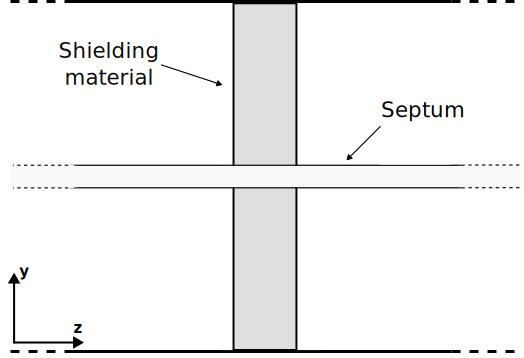
\includegraphics[width=\textwidth]{content/img/ASTM ES7-83.png}
        \caption{Shielding material in TEM cell}
        \label{fig:ASTM ES7-83}
    \end{subfigure}%
    \hfill
    \begin{subfigure}[h]{0.49\textwidth}
        \centering
        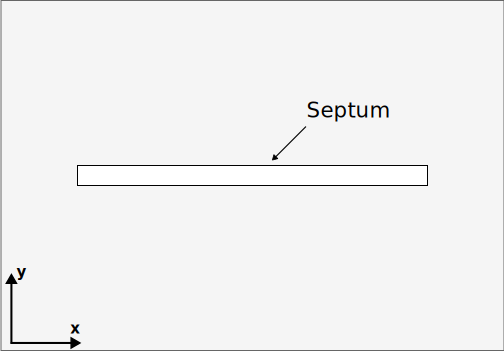
\includegraphics[width=\textwidth]{content/img/form_of_shielding_material.png}
        \caption{Shape of the shielding material}
        \label{fig:form_of_shielding_material}
    \end{subfigure}
    \label{fig:subfigures}
\end{figure}

Then, the S-parameters derived in the simulations are used to get to the output powers $P_\mathrm{ref}$ and $P_\mathrm{load}$. By exciting the TEM cell with a power of 1\,W, the reference power $P_\mathrm{ref}=1\,\mathrm{W}$. The measured power is then derived through

\begin{equation}
    P_\mathrm{load}=P_\mathrm{ref}\cdot10^{|S_\mathrm{12, dB}|/10}.
    \label{eqn:load_power}
\end{equation}

\subsubsection{Dual TEM cell}\label{sec:dual_tem_cell}

The shielding effectiveness of a material may also be determined using a dual TEM cell shown in \autoref{fig:dual_tem_cell}. They are connected through an aperture, which can be filled with the shielding material or left empty. The upper TEM cell is excited through port 1, and acts as a driving cell, transmitting power through the aperture. Port 2 is loaded with the reference impedance $Z_w\approx50\,\Omega$. The second TEM cell functions as a receiver, collecting power at its output ports \cite{MORARI_BĂLAN_2015}.

\begin{figure}[h]
	\centering
	\includegraphics[width=0.75\linewidth]{content/img/dual_tem_cell.png}
	\caption{Dual TEM cell with aperture}
	\label{fig:dual_tem_cell}
\end{figure}

If the aperture is electrically small, its coupling may be described by an electric and a magnetic dipole moment. Their magnitude is related to the electric and magnetic coupling between the TEM cells over the aperture. Therefore, the electric and magnetic coupling can be determined separately by adding or subtracting the output powers of the receiving TEM cell \cite{MORARI_BĂLAN_2015, 4091811}. Consequently, a electric shielding effectiveness $SE_\mathrm{dB}^\mathrm{e}$ and a magnetic shielding effectiveness $SE_\mathrm{dB}^\mathrm{m}$ can be calculated with

\begin{subequations}
	\begin{equation}
		SE_\mathrm{dB}^\mathrm{e}=10\log{\left( \frac{P_\mathrm{ref, sum}}{P_\mathrm{load,sum}} \right)},
		\label{eqn:se_dual_cell_e}
	\end{equation}
	\begin{equation}
		SE_\mathrm{dB}^\mathrm{m}=10\log{\left( \frac{P_\mathrm{ref, diff}}{P_\mathrm{load,diff}} \right)}.
		\label{eqn:se_dual_cell_m}
	\end{equation}
\end{subequations}

Separating the electric and magnetic shielding effectiveness is useful when applying shielding materials in the near field of electric or magnetic dipole moments. For shielding a magnetic dipole moment, the $SE_\mathrm{dB}^\mathrm{m}$ value is considered significant \cite{4091811}, whereas for an electric dipole moment, the $SE_\mathrm{dB}^\mathrm{e}$ value is relevant.

%Because the normalized electric field at the aperture will be of TEM mode, only the component normal to the aperture in z-direction has to be considered. Just as in the case of dipole representation, the Lorentz Reciprocity theorem may be applied to find the fields in the TEM cell. Because both the fields at the output and in the aperture are of TEM mode, only the E-field at the output may be considered. 





\section{Finite Element Method}\label{sec:simulations}
\subsection{Finite Element Method}

\subsubsection{General Idea}
Problems involving the calculations of electromagnetic fields are often cumbersome and difficult to solve. This is due to the need of solving differential equations describing these fields over a computational domain, which is not possible with a computer in this sense. The simulation software Ansys HFSS (High Frequency Simulation Software) aims to provide a solution. This software is used for the simulations in \autoref{sec:simulations}, hence it is described in this following, dedicated section.

HFSS uses a numerical technique, namely the Finite Element Method (FEM). The general idea of FEM after Rayleigh-Ritz-Galerkin is to choose a number of basis functions. The goal is to find a linear combination of these basis functions, so that the differential equation is satisfied as closely as possible. This turns the problem of solving a differential equation into a system of algebraic equations, which the computer can process. There is always a set of basis functions which enable the calculation to converge to the real solution. However, the number of basis functions used in the domain is limited, due to reasons of computability \cite{STRANG_2018}. 

FEM therefore divides the domain into finite elements, i.e. smaller pieces. Then, within each piece, such a basis function is assigned. A linear combination of these basis functions are found, which satisfy the differential equations. In region where the approximating solution has a high degree of error, the accuracy may be increased by further subdividing the finite elements. This is repeated, until the error falls below a certain threshold, and a precise solution is derived.

\subsubsection{Dividing a computational domain into finite elements}

The differential equation to be solved is shown in \autoref{eqn:full_wave_equation}, where $\epsilon_r$ is the relative permeability and $\mu_r$ is the relative permeability of the material. The variable $k_0$ is the wave number of free space and equals $k_0=\omega\sqrt{\epsilon_0\mu_0}$. \cite{Cendes_Lee_1988,85399,Cendes_1991}.

\begin{equation}
    \nabla\times\left(\frac{1}{\mu_r}\nabla\times\mathbf{E}\right)-k_0^2\epsilon_r\mathbf{E}=0 \quad\text{in $\Omega$}
    \label{eqn:full_wave_equation}
\end{equation}

This equation is solved in a computational domain $\Omega$. This computational domain is divided into finite elements, called a mesh. Each node in this mesh has polynomial functions assigned, which are weighted to approximate the real solution. It has been proven that tetrahedral finite elements are best suited for this task, as they are geometrically flexible and make the definition of complete polynomial approximation functions possible \cite{Shenton_Cendes_1985}. Ansys HFSS uses a adaptive finite element mesh generator, which automatically provides a mesh for a given 3-dimensional construction. The Delaunay tesselation for three-dimensions is used for generating a mesh. It efficiently creates a mesh from objects of arbitrary shapes. Any boundary condition can be added recursively to the mesh. At the heart of this algorithm lies the property, that the circumsphere of an tetrahedra's vertices may not contain other tetrahedra's vertices. 

\autoref{fig:tetrahedral_mesh} shows one of such tetrahedrons. At the edge points, the components of the field which are normal to the respective edge and tangential to the face of the element is stored. At the vertex points, the component of a field which are tangential to the edges are stored. The value of the field at any midpoint is derived through interpolation from the node values. The basis function is used for interpolation.

\begin{figure}[h]
    \centering
    \includegraphics[width=0.25\linewidth]{content/img/tetrahedral_mesh.png}
    \caption{Tetrahedron with points on the edge and vertices.}
    \label{fig:tetrahedral_mesh}
\end{figure}

Because of the way how the fields are stored in the tetrahedra, they are called tangetial vector finite elements. Their advantage is that tangential components of fields can be forced to be equal among adjacent tetrahedra at the boundary. For example, an electric field stored at a vertex point must point in the direction along one of the edges, therefore it is tangential to the element. An adjacent element then has the same tangential electric field imposed at this node, leading to a continuous tangential electric field, therefore satisfying the boundary conditions implied by the Maxwell equation automatically. Furthermore, any Dirichlet boundary conditions can easily be set along the edges.
\cite{85399}. 

The finite element is described as \autoref{eqn:finite_element_3d}, where $L_2(\Omega)$ is a set of square integrable functions and $P_1$ a set of piecewise linear functions in the discretized domain $\Omega$ \cite{104986}. The vector fields at the vertices are given as $u$. $D(\Omega)$ is a set of divergence free functions. The vectors $u$ used in the finite element therefore 

\begin{itemize}
    \item are continuous in the normal direction.
    \item are square integrable.
    \item have a curl describable by piecewise linear functions.
\end{itemize}

\begin{equation}
    H^{(\dim=3)}_1(\mathrm{curl}) = \left\{ \mathbf{u} \mid \mathbf{u} \in \left[ L_2(\Omega) \right]^3, \nabla \times \mathbf{u} \in \left[ P_1(\Omega) \right]^3 \cap D(\Omega) \right\}
    \label{eqn:finite_element_3d}
\end{equation}

\autoref{fig:tetrahedra_w_unknowns} shows the finite element with the unknowns marked at each point. For reasons of simplicity, only the face is shown. The variables $u_i^j$ and $u_j^i$ are imposed across element boundaries, therefore guaranteeing tangential continuity at boundaries. Additionally, they inherently defined a linear polynomial, meaning that they describe a gradient of the field along this edge. \autoref{eqn:tangential_vector_component} describes this relation mathematically, where $\mathbf{t}_{ij}$ is the unit vector tangentially to the edge from node i to node j and $l_{ij}$ is the length of this edge.

\begin{equation}
    \mathbf{u}\cdot\mathbf{t}_{ij}=\frac{1}{l_{ij}}\left( u_i^j-u_j^i \right)
    \label{eqn:tangential_vector_component}
\end{equation}

\begin{figure}[h]
    \centering
    \includegraphics[width=0.25\linewidth]{content/img/tetrahedra_w_unknowns.png}
    \caption{Face of the finite element with unknowns}
    \label{fig:tetrahedra_w_unknowns}
\end{figure}

Two facial unknowns $f_1$ and $f_2$ are added to two of the three edge points at one face. Contrary to the variables $u_i^j$, the facial unknowns $f_i$ are only assigned locally at each element and do not cross boundaries. The purpose of the facial unknowns $f$ is to provide a quadratic polynomial for the field component normal to the edges. This will lead to a linear approximation for the curl of the unknown vector field $\nabla\times \mathbf{u}$, providing sufficient accuracy. The overall vector field of this element is then calculated by a superposition of all nodes' vector attributions.

\subsubsection{Solving the differential equation}

A testing function $\mathbf{W}_n$ is defined, which is multiplied to \autoref{eqn:full_wave_equation}. Integrating over the whole test volume then leads to \autoref{eqn:test_funct}. This yields $N$ equations, with $n=1,2,...N$, for each finite element in the domain $\Omega$. This is a common procedure in FEM, and it works through orthogonalization of the residual of \autoref{eqn:full_wave_equation} with respect to the function $\mathbf{W}_n$. This means the new goal of the solution is to minimize the residual by making $\mathbf{W}_n$ as orthogonal as possible \cite{Mohsen_1982}.

\begin{equation}
    \int_\Omega\left( \mathbf{W}_n\cdot\nabla \times\left( \frac{1}{\mu_r}\nabla\times\mathbf{E} \right)-k_0^2\epsilon_r\mathbf{W}_n\cdot\mathbf{E} \right)\mathrm{d}V=0
    \label{eqn:test_funct}
\end{equation}

Using the vector identity $\nabla\cdot\left(\mathbf{a}\times\mathbf{b}\right)=\left(\nabla\times\mathbf{a}\right)\cdot\mathbf{b}-\mathbf{a}\cdot\left(\nabla\times\mathbf{b}\right)$  on \autoref{eqn:test_funct} provides a weak form of the equation, meaning a form of the original partial differential equation, which does not contain all original derivatives \cite{Cendes_Lee_1988,Cendes_1991}. Additionally, boundary terms come into play, as seen in the right hand side of the resulting \autoref{eqn:greens_theorem_wave_eqn}. The usefulness in this step has been described as lowering the highest-order derivative, therefore the approximating functions need to guarantee continuity of value, not of slope \cite{huebner2001finite}. Another explanation is the possibility of incorporation of Neumann boundary conditions \cite{Mohsen_1982}. 

\begin{equation}
    \int_\Omega \left[ \left(\nabla \times \mathbf{W}_n \right)\cdot \frac{1}{\mu_r}\nabla\times \mathbf{E}-k_0^2\epsilon_r\mathbf{W}_n\cdot\mathbf{E}\right]\mathrm{d}V=\underbrace{\oint_{\partial\Omega}\left( \mathbf{W}_n\times \frac{1}{\mu_r}\nabla\times\mathbf{E}\right)\cdot\mathrm{d}\mathbf{S}}_{\text{Boundary term}}
    \label{eqn:greens_theorem_wave_eqn}
\end{equation}

Next, the electric field $\mathbf{E}$ is represented by a superposition of basis functions. When applying Galerkin's method, the basis functions are equal to the test functions $W_n$. \autoref{eqn:representation_e_field_fem} demonstrates the sum of the basis functions, which are weighted with the variable $x_m$. These variables $x$ for all elements have to be solved, to find the electric field $\mathbf{E}$ over the whole domain. The FEM has therefore reduced the initial wave equation in \autoref{eqn:full_wave_equation} to a simple linear matrix equation $Ax=b$, where $A$ is a known $N\times N$ matrix, $b$ contains port excitations and $x$ is the unknown. Ideally, the basis functions are defined to be zero outside of their adjacent elements. This will result to zero for all entries in the matrix, where the test and basis function do not overlap. Therefore, the matrix is sparse, and will be solved much faster. In the end, other electromagnetic quantities can all be derived through the electric field.

\begin{equation}
    \mathbf{E}=\sum^N_mx_m\mathbf{W}_n
    \label{eqn:representation_e_field_fem}
\end{equation}

\autoref{eqn:matrix_a} shows what the matrix then looks like. Some manipulation on the boundary term have been made, so that it contains the surface impedance $Z_s$. The surface impedance defines the ratio of the electric field to the magnetic field on the boundary region. Furthermore, it contains the free space, which equals $\eta_0 \approx 377\,\Omega$.

\begin{equation}
A_{ij} = \int_{\Omega} \nabla \times \mathbf{W}_i \, \frac{1}{\mu_r} \nabla \times \mathbf{W}_j \, \mathrm{d}V 
- k_0^2 \int_{\Omega} \mathbf{W}_i \, \varepsilon_r \mathbf{W}_j \, \mathrm{d}V 
+ \mathrm{i} k_0 \left(\frac{\eta_0}{Z_s}\right) \oint_{\partial\Omega} \mathbf{n} \times \mathbf{W}_i \cdot \mathbf{n} \times \mathbf{W}_j \, \mathrm{d}\mathbf{S}
\label{eqn:matrix_a}
\end{equation}

\subsubsection{Adaptive solution process}

Each finite element therefore has a solved electric field assigned, which should approximate the real solution as closely as possible. To determine the error for each element, \autoref{eqn:full_wave_equation} is evaluated. The elements with the highest residuals contain the largest deviation from the real result, meaning they have a large degree of error. Region in the mesh with large degrees of errors are refined, i.e. the tetrahedral finite elements are split into smaller ones. This allows the FEM solver to recalculate the fields in this region with higher precision, leading to a smaller residual. Consequently, the finite elements represent the fields more accurately, due to a smaller element size and higher resolution \cite{1063929}. An additional method is increasing the order of the polynomial basis functions of elements with low degree of accuracy.

\begin{equation}
    \nabla\times\left(\frac{1}{\mu_r}\nabla\times\mathbf{E}_{\mathrm{solved}}\right)-k_0^2\epsilon_r\mathbf{E}_{\mathrm{solved}}=residual
    \label{eqn:full_wave_equation_solved}
\end{equation}

To determine when the iterative refinement process is done and the solution good enough, some kind of threshold must be defined. One possibility is the $\mathrm{Max}\ \Delta \mathrm{S}$ parameter. It is compared to the difference of S-parameters of the defined excitation ports over two iterations. If, after a mesh refinement, the S-parameters of the ports do not significantly change anymore, meaning change less than $\mathrm{Max}\ \Delta \mathrm{S}$, then the iterative process can be considered done. This described iterative process is shown in \autoref{fig:workflow_fem}. 

\begin{figure}[h]
    \centering
    \includegraphics[width=0.75\linewidth]{content/img/workflow_fem.png}
    \caption{Adaptive solution process}
    \label{fig:workflow_fem}
\end{figure}

\todo{Short HFSS introduction with boundary conditions, ports and modal and terminal solutions?}
 % Fehlende Ressourcen von Zoltan in Journal of Applied Physics. Schreibe über mathetmaische Grundlagen, Meshing, Dipole Excitation und Impedance Network Boundary Counditions (INBC)

% Additional missing ressource: Finite Elements, Electromagnetics, and Design



\subsection{Investigation of antennas}
\subsubsection{Conceptual framework and modeling}

\todo[inline]{Einige Themen hier sollten zum Theorieteil voriger Kapitel verschoben werden.}

\begin{figure}[h]
	\centering
	\includegraphics[width=0.7\linewidth]{content/img/antenna_port}
	\caption{Geometry of an antenna's feedpoint used in simulation. The antenna is fed through a waveport. This geometry leads to a port impedance of $50\,\Omega$.}
	\label{fig:antennaport}
\end{figure}


The coupling of various electrically small antennas placed in a TEM cell is investigated. Their electric and magnetic coupling is investigated through dipole moments. All antennas are fed with a power of 1\,W. Their material are made of a perfect electric conductor. Different positions and offsets are investigated and the results discussed. They are fed through a round wave port with a diameter of 0.46\,mm, and their wire has a diameter of 0.2\,mm and free-space permittivity. This results in a reference impedance of $Z_0\approx 50$\,$\Omega$. The TEM cell used has a width of $a=40$\,mm, a height of $b=24$\,mm and a length of $l=100$\,mm, and its cells walls and septum consist of a perfect electric conductor, too. The TEM cell model does not contain the tapered sections at the ports. The ports have an impedance of $50\,\Omega$ due to the TEM cell's geometry.


\begin{figure}[htbp]
	\centering
	\begin{subfigure}[b]{0.48\textwidth}
	\centering
\includegraphics[width=1\linewidth]{content/img/tem_cell_front}
\caption{xy-plane}
\label{fig:temcellfront}
	\end{subfigure}
	\hfill
	\begin{subfigure}[b]{0.48\textwidth}
	\centering
\includegraphics[width=1\linewidth]{content/img/tem_cell_side}
\caption{yz-plane}
\label{fig:temcellside}
	\end{subfigure}
	
	\caption{Geometrical arrangement of the TEM cell used in simulations. The front shows the xy-plane, and the side the yz-plane of the TEM cell.}
	\label{fig:example}
\end{figure}

The capacitance and inductance of the TEM cell is derived by calculating the feed current and voltage out of the S-parameters. The capacitance and inductance are then derived through the electric and magnetic peak energy. The values fluctuate slightly over frequency by $\pm1\,\%$, which is likely due to numerical inaccuracies. The average capacitance and inductance values over the frequency range are chosen. It is therefore assumed that the TEM cell has a constant capacitance and inductance. $C_T = 6.74\,\mathrm{pF}$, $L_T = 16.25\,\mathrm{nH}$. 

The coupling between the antenna and the two ports of the TEM cell are described by S-parameters, specifically the forward transmission coefficients $S_{\mathrm{A1}}$ and $S_{\mathrm{A2}}$. The magnitude of this coefficient is the same for the antenna to both ports ($|S_{\mathrm{A1}}|=|S_{\mathrm{A2}}|$). The power transferred from the antenna $P_{\mathrm{Antenna}}$ to the output ports $P_{\mathrm{Out1}}$ and $P_{\mathrm{Out2}}$ is then derived through

\begin{equation}
	P_{\mathrm{Antenna}}=\frac{P_{\mathrm{Out1}}}{10^{|S_{\mathrm{A1}}|/10}}=\frac{P_{\mathrm{Out2}}}{10^{|S_{\mathrm{A2}}|/10}}.
	\label{eqn:power_antenna}
\end{equation}

The fields are normalized such that 

\begin{equation}
	\iint_S \mathbf{E}^\pm \times \mathbf{H	_0}\pm \cdot d\mathbf{s}' = 1,
	\label{eqn:normalization of fields}
\end{equation}

where the surface $S$ spans over one of the output ports. The fields are linearly scaled by the complex coefficients $a$ and $b$. If only the TEM mode is considered, only one such pair of coefficients is needed to describe the fields at the output ports. Some investigations explicitly include the propagation of higher order modes. In this case, each mode is assigned a separate pair of coefficients $a_n$, $b_n$. The coefficients $a$ and $b$ have the unit $\sqrt{\mathrm{W}}$.

%\begin{figure}[h]
%	\centering
%	\includegraphics[width=1\linewidth]{content/img/sketch_dipoles_tem_cell.png}
%	\caption{Dipole moments and measurement point of $e_{0,z}$ in TEM cell}
%	\label{fig:sketch_dipoles_tem_cell2}
%\end{figure}

The coefficients $a$ and $b$ have the unit $\sqrt{\mathrm{W}}$. The fields $\mathbf{e_0}$ and $\mathbf{h_0}$ for a TEM cell is known \todo{Some plot or table for explanation}.The normalization condition leads to an output power equal to $P_\mathrm{out,1} = |a|^2/2$ and $P_\mathrm{out,2}=|b|^2/2$, which is also found in \cite{4091811}. This is derived by

\begin{subequations}
	\begin{equation}
		P_{\mathrm{out1}}=\iint_S \langle \mathbf{S} \rangle \cdot \mathrm{d}\mathbf{s'}= \iint_S \frac{1}{2} \, \Re \{ \left(a\cdot \mathbf{E}^\pm\right) \times \left(a\cdot \mathbf{H}^\pm\right)^* \}\cdot \mathrm{d}\mathbf{s'} = \frac{|a|^2}{2},
		\label{eqn:power_of_poynting1}
	\end{equation}
	\begin{equation}
		P_{\mathrm{out2}}=\iint_S \langle \mathbf{S} \rangle \cdot \mathrm{d}\mathbf{s'}= \iint_S \frac{1}{2} \, \Re \{ \left(b\cdot \mathbf{E}^\pm\right) \times \left(b\cdot \mathbf{H}^\pm\right)^* \}\cdot \mathrm{d}\mathbf{s'} = \frac{|b|^2}{2}.
		\label{eqn:power_of_poynting2}
	\end{equation}
\end{subequations}

Because ideal TEM fields are assumed at the output ports, the Poynting vector has no imaginary component,


\begin{equation}
	\mathbf{E}^\pm\times\mathbf{H}^\pm=\Re\{\mathbf{E^\pm}\times\left(\mathbf{H}^\pm\right)^*\} \quad\text{for TEM mode}.
	\label{eqn:equivalent_tem}
\end{equation}

Consequently, if the normalized electric field distribution of the TEM mode $\mathbf{E^\pm}$ is unknown, it may be derived by setting the output power of a waveport to $P_{\mathrm{out}}=1/2\,\mathrm{W}$, where $|a|=|b|=1\,\sqrt{\mathrm{W}}$. For example, the uniformly distributed, normalized electric field along the y-axis in the center of the TEM cell ($z=0$, $x=0$) is derived by

\begin{equation}
	|a|\cdot\mathbf{E}^\pm(0,y,0)=1\sqrt{\mathrm{W}}\cdot\mathbf{E}^\pm = \frac{\sqrt{P_\mathrm{out}R_\mathrm{waveport}}}{b/2}
\end{equation}
 
 The difference in phase of $S_{\mathrm{A1}}$ and $S_{\mathrm{A2}}$ influence the quantity of magnetic dipole moments and electric dipole moments.  If the dipole moments are placed in the center of the TEM cell half-way between both output ports, they will contain the same power, therefore $|a| = |b|$. In this case, a phase shift of $\pi$ indicates the presence of a magnetic dipole moment and the absence of electric dipole moments. This is shown by

\begin{subequations}
	\begin{equation}
		\mathbf{m}_\mathrm{e} = \frac{a+b}{\mathbf{E}^\pm} = \frac{a+a\cdot e^{j\pi}}{\mathbf{E}^\pm} = 0,
	\end{equation}
	\begin{equation}
		\mathbf{m}_\mathrm{m} = j\frac{a-b}{\mathbf{E}^\pm\cdot k_0} = j\frac{a-a\cdot e^{j\pi}}{\mathbf{E}^\pm\cdot k_0} = j\frac{2a}{\mathbf{E}^\pm\cdot k_0}.
	\end{equation}
\end{subequations}

 A phase shift of zero indicates the opposite case. The influence of the electric and magnetic dipole moment is equal, if the phase shift equals $\pi/2$. 

If only the TEM mode propagates, only the y-component of an electric dipole moment and the x-component of a magnetic dipole moment generates output power, assuming they are centrally located ($x=0$, $y=b/4$, $z=0$). This is due to the magnetic field containing only an x-component $\mathbf{H}^\pm = H_x^\pm e^{\pm k_0 z}$, and the electric field only an y-component $\mathbf{E}^\pm = E_y^\pm e^{\pm k_0 z}$ at the center of the TEM cell. \todo{Sketch this situation. Also, $e^{\pm k_0 z}$ indicated that at z=0 the dipole moment is located. Consider this in all sketches}
An offset of dipole moments or propagation of higher order modes lead to different field components of $\mathbf{H}^\pm$ and $\mathbf{E}^\pm$, and therefore to a change in coupling. These effects are investigated numerically in \autoref{sec:dipole_moments}.

A magnetic dipole moment can be expressed equivalently as either an electric current loop or a magnetic line current, as described in \autoref{eqn:magn_current_curr_loop}. For infinitesimal magnetic dipoles, this duality simplifies to
\begin{equation}
	m_{\mathrm{m}}=j\omega\mu_0 m_{\mathrm{0}},
	\label{eqn:m_mymag_ifa}
\end{equation}
where $m_{\mathrm{m}}$ (in V$\cdot$m) denotes the magnetic dipole moment in the magnetic current representation, and $m_{\mathrm{0}}$ (in A$\cdot$m$^2$) denotes the moment in the electric current representation.

If the output power and phase shifts of the waveports are known, any antenna in the TEM cell may be replaced by an electric and a magnetic dipole moment. Using numeric simulation, the phase shift is determined by measuring the phase shifts of the electric fields at both output ports. When applying this described method in a measurement with a real TEM cell, the phase shift is found by adding and subtracting the output powers of both ports, as is shown in \cite{Sreenivasiah_Chang_Ma_1981}.

The energy density is given by \cite[p. 330]{Griffiths_2024}

\begin{equation}
	w_\mathrm{EM} = \frac{1}{2}\left(\underbrace{\epsilon E^2}_{\text{Electric energy} w_E} + \underbrace{\frac{1}{\mu} B ^ 2}_{\text{Magnetic energy} w_M}\right).
	\label{eqn:em_energy}
\end{equation}

Integrating $w_\mathrm{EM}$ over a volume yields the total electromagnetic energy in this volume. Similarly, integrating $w_E$ gives the electric energy in said volume, and $w_M$ the magnetic energy.

If all of the energy is provided by an electrically short antenna, its equivalent reactances can be derived through \cite[pp 107, 328]{Griffiths_2024}

\begin{subequations}
	\begin{equation}
		L = 2\frac{W_m}{I^2}
		\label{eqn:m_energy}
	\end{equation}
	\begin{equation}
		C = 2 \frac{W_e}{V^2}
		\label{eqn:e_energy}
	\end{equation}
\end{subequations}


All simulations are counterchecked by inserting frequency-dependent dipole moments and checking the power and phase of the output ports.

In the measurement configuration, the TEM cell with an inserted antenna can be modeled as a three-port network. The two output ports of the TEM cell are denoted as ports 1 and 2, while the antenna feed point is represented as port A. The behavior of this system is fully characterized by its scattering matrix, given as

\begin{equation}
	\left[S\right]=
	\begin{bmatrix}
		S_{11} & S_{12} & S_{1A} \\
		S_{21} & S_{22} & S_{2A} \\
		S_{A1} & S_{A2} & S_{A}
	\end{bmatrix}.
\end{equation}

 The current through the feedpoint of the antennas are calculated with those S-parameters,
 
 \begin{equation}
 	I_{in} = \sqrt{P_{in}}\frac{(1-S_{AA})}{\sqrt{Z_0}},
 \end{equation}
 
  $P_{in}$ is the power applied to the port, not considering reflections. The voltage at the feedpoint is calculated in a similar fashion as 
 
 \begin{equation}
 	V_{in} = \sqrt{P_{in}}(1-S_{AA})\sqrt{Z_0}.
 \end{equation}
 
 The impedance seen from the feedpoint is 
 
 \begin{equation}
 	Z_{in}=Z_0\frac{1+S_{AA}}{1-S_{AA}}.
 \end{equation}
 

\FloatBarrier
\subsubsection{Monopole Antenna}
\subsubsection{Setup}
\FloatBarrier

\begin{figure}[htbp]
	\centering
	\hspace*{-0.0cm}
	\begin{subfigure}[b]{0.48\textwidth}
		\centering
		\includegraphics[height=8cm]{content/img/monopole_near_field}
		\caption{}
		\label{fig:monopolenearfield}		
	\end{subfigure}
	\hfill
	\begin{subfigure}[b]{0.48\textwidth}
		
		\centering
		\raisebox{0.12cm}{\includegraphics[height=8cm]{content/img/monopole_antenna}}
		\caption{}
		\label{fig:monopoleantenna}
	\end{subfigure}
	
	\caption{Geometry of monopole antenna inserted into TEM cell with its electric near-field.}
	\label{fig:field_monopole_antenna}
\end{figure}


The monopole antenna, shown in \autoref{fig:monopoleantenna}, is installed at the center of the TEM cell and connected to the feedpoint located on the top wall. It has a length of 5\,mm, which makes it electrically short at frequencies up to 6\,GHz. It may be approximated as an infinitesimal electric dipole for frequencies up to 1.25\,GHz. The equivalent dipole moments $\mathbf{m}_e$ and $\mathbf{m}_m$ are derived through \cref{eqn:ifa_me, eqn:ifa_mm}. 

The frequency range investigated reaches from 1\,MHz to 3\,GHz. \autoref{fig:te01_te10_tem_propagation} demonstrates the cut-off frequencies of higher-order modes of the TEM cell in use for the simulation, where the cut-off frequency of TE\textsubscript{01} equals $f_{\mathrm{c,01}}=3.12\,\mathrm{GHz}$. The output power is influenced by the propagation of this evanescent mode, which must be considered in the simulation results in the upper frequency range. 


\FloatBarrier
\subsubsection{Equivalent dipole moments}
\FloatBarrier



The electric dipole moment is normalized to the free-space wave impedance to enable comparison with the magnetic dipole moment \cite{Kreindl_Bauernfeind_Weiss_Stockreiter_Kaltenbacher_2024}. The electric dipole moment shown in \autoref{fig:dipole_moments_monopole} increases approximately linearly over frequency, while the magnetic dipole moment is negligible over the whole frequency range. Consequently, the phase difference between the powers $\Delta = \varphi_2 - \varphi_1=0$ over the whole frequency range. 

\begin{figure}[htbp]
	\centering
	\begin{subfigure}[b]{0.48\textwidth}
		\centering
		\includegraphics[width=1\linewidth]{content/img/dipole_moments_monopole.png}
		\caption{Dipole moments}
		\label{fig:dipole_moments_monopole}
	\end{subfigure}
	\hfill
	\begin{subfigure}[b]{0.48\textwidth}
		\centering
		\includegraphics[width=1\linewidth]{content/img/phase_shift_monopole}
		\caption{Phase shift}
		\label{fig:phaseshiftmonopole}
	\end{subfigure}
	
	\caption{The equivalent dipole moments of the monopole antenna and the corresponding induced phase shift between the wave ports are presented in separate figures.}
	\label{fig:monopole_moments_phase}
\end{figure}

\FloatBarrier
\subsubsection{Electrical characteristics}
\FloatBarrier

\begin{figure}[htbp]
	\centering
	\begin{subfigure}[b]{0.48\textwidth}
		\centering
		\centering
		\includegraphics[width=1\linewidth]{content/img/monopole_feed_voltage}
		\caption{Voltage at feedpoint}
		\label{fig:monopolefeedvoltage}
	\end{subfigure}
	\hfill
	\begin{subfigure}[b]{0.48\textwidth}
		\centering
		\includegraphics[width=1\linewidth]{content/img/monopole_feed_current}
		\caption{Current at feedpoint}
		\label{fig:monopolefeedcurrent}
	\end{subfigure}
	
	\caption{Current and voltage at feedpoint of monopole antenna over frequency.}
	\label{fig:example}
\end{figure}

\todo{axis typo}

The electric current present in the monopole antenna is aligned with the electric field $\mathbf{e}_\mathrm{TEM}^\pm$ of the dominant TEM mode present in the investigated frequency range. Only the the electric dipole moment in y-direction and the magnetic dipole moment in x-direction are needed to model the antenna, because they align with the fields of the TEM mode.

According to \autoref{eqn:J1_propagating_waves}, this will lead to a coupling with the output ports. \autoref{eqn:J1_propagating_waves} also requires $\mathbf{e}_\mathrm{TEM}^\pm$ and the part of $I$ contributing to the output power to be in phase at the position of the monopole antenna, due to $\mathbf{e}_\mathrm{TEM}^\pm$ and $\mathbf{h}_\mathrm{TEM}^\pm$ being in-phase at the output ports. Using \cref{eqn:e_int_a, eqn:e_int_b} and integrating the current $I$ in \autoref{fig:monopolefeedcurrent} yields

\begin{equation}
	\mathbf{m}_e=\int_C \boldsymbol{\tau} I(l)\,dl = 82.00\,\mu\mathrm{Am}\cdot\mathbf{\hat{a}}_z,
\end{equation}

which is equivalent to $\mathbf{m_e}=3.09\cdot 10^{-2} \cdot\mathbf{\hat{a}}_z\,\mathrm{Vm}$, if normalized to the free-space wave impedance $Z_0\approx 376.73\,\Omega$. Since the monopole antenna is located in the center, $\mathbf{e}_\mathrm{TEM}^\pm$ remains constant over $y$.

%For example, measuring the y-component of the electric field at the center of output port 1 yields $E_y^+(x=0, y, z=l/2)=15.35\,\mathrm{V/m}$, which is constant over $y$. \todo{differentiate somehow between normalized and normal electric field}. Using the Lorentz Reciprocity theorem \autoref{eqn:J1_propagating_waves}, and integrating $E_y^+(x=0, y, z=l/2)$ and $I(x=0, y, z=l/2)$ over the length of the monopole antenna yields \todo{all values must be peak values}

%\begin{equation}
%	\int_C E_y^+(x=0, y, z=l/2)\cdot I(x=0, y, z=l/2)\,dy=521.9\,\mathrm{\mu W}=2a^2.
%\end{equation}
%
%Applying \autoref{eqn:ifa_me} to then derive the electric dipole moment leads to 
%
%\begin{equation}
%	\mathbf{m}_e = \sqrt{2}\frac{521.9\,\mathrm{W}}{\mathbf{E^\pm}}=
%\end{equation}




The voltage $V$ at the feedpoint in \autoref{fig:monopolefeedvoltage} remains largely constant over the frequency range. This agrees with the absence of magnetic dipole moment $\mathbf{m}_m$, which is directly related to induced voltage according to \autoref{eqn:m_v}. The current $I$ at the feedpoint in \autoref{fig:monopolefeedcurrent} rises linearly. According to \autoref{eqn:me_i}, the frequency behavior of $\mathbf{m}_\mathrm{e}$ is proportional to $I$. \autoref{eqn:me_i} cannot directly be applied using $I$, because some of this current returns as displacement current to the feedpoint (see \autoref{fig:monopolenearfield}), not contributing to the electric coupling. Furthermore, this agrees with the quadratically increasing output power in \autoref{fig:monopoleoutputpower} and the quadratically increasing radiation resistance determined.

\begin{figure}[htbp]
	\centering
	\begin{subfigure}[t]{0.48\textwidth}
		\centering
		\includegraphics[height=5cm]{content/img/monopole_output_power}
		\caption{Output electric field and power of monopole antenna.}
		\label{fig:monopoleoutputpower}
	\end{subfigure}
	\hfill
	\begin{subfigure}[t]{0.48\textwidth}
		\centering
		\includegraphics[height=5cm]{content/img/monopole_moment_comp}
		\caption{Comparison of output power produced by monopole antenna and equivalent dipole moments.}
		\label{fig:monopolemomentcomp}
	\end{subfigure}
	
	\caption{Output power and electric field data of antenna and equivalent dipole moments}
	\label{fig:monopole_power_comp}
\end{figure}

The derived equivalent dipole moments $\mathbf{m}_e$, $\mathbf{m}_m$ positioned in the center of the TEM cell produce output power shown in \autoref{fig:monopolemomentcomp}, where they are compared with the monopole antenna. The approximation with the dipole moments worsens, when approaching the cut-off frequency of the first higher-order mode. The coefficients $a_{01}$ and $b_{01}$ of the TE\textsubscript{01} have to be considered, which would provide the difference in power to increase accuracy.

The output power rises quadratically over the frequency, which fits the linearly rising electric dipole moment and the quadratically rising radiation resistance determined in section \todo{Fill in}.




\begin{figure}[htbp]
	\centering
	\begin{minipage}[t]{0.48\textwidth}
		\centering
		\centering
		\includegraphics[width=1\linewidth]{content/img/monopole_current_dist}
		\caption{At $3\,\mathrm{GHz}$}
		\label{fig:currentdistributionmonopole}
		\hfill
	\end{minipage}
	\hfill
	\begin{minipage}[t]{0.48\textwidth}
		\centering
		\includegraphics[width=1\linewidth]{content/img/current_loop_charge_distribution_1MHz}
		\caption{At $1\,\mathrm{MHz}$}
		\label{fig:currentloopchargedistribution1mhz}
	\end{minipage}
	\caption{Current distribution along the monopole antenna at frequencies $1\,\mathrm{MHz}$ and $3\,\mathrm{GHz}$}
	\label{fig:monopole_current_dist}
\end{figure}






The distribution of the current along the monopole antenna shown in \autoref{fig:monopole_current_dist} is numerically derived by integrating the magnetic field intensity in a closed loop around the antenna at each position. 

Near the feedpoint at $0\,\mathrm{mm}$ non-linearities become apparent, due to significant displacement current in this region, as \autoref{fig:monopolenearfield} makes clear. This causes the current in the antenna to rapidly decreases in this section. 

The current distribution at $3\,\mathrm{GHz}$ (see \autoref{fig:currentdistributionmonopole}) approximates that of a small electric dipole as described in \autoref{sec:small_electric_dipole}. It shows an approximately linear decrease. Any current observed beyond the antenna length of $5\,\mathrm{mm}$ is attributed to displacement current to the septum, as is visible by the increased electric field there in \autoref{fig:monopolenearfield}.

The current distribution at $1\,\mathrm{MHz}$ demonstrated in \autoref{fig:currentloopchargedistribution1mhz} approximately follows the behavior of an infinitesimal electric dipole discussed in \autoref{sec:infinitesimal_electric_dipoles}. There, the current remains nearly constant over some sections of antenna length, decreasing towards the end. Additionally, the magnitude of the current is significantly lower at this frequency. 

\begin{figure}
	\centering
	\includegraphics[width=0.4\linewidth]{content/img/monopole_imp}
	\caption{Magnitude and phase of monopole antenna's impedance.}
	\label{fig:monopoleimp}
\end{figure}


This frequency-dependent behavior is explained by the impedance of the monopole antenna shown in \autoref{fig:monopoleimp}. At low frequencies, the antenna impedance demonstrates a high magnitude, which rapidly decreases as frequency increases. Over the whole frequency range, it exhibits highly capacitive behavior, which is consistent with \autoref{eqn:compl_power_inf_elec_dipole}.


An equivalent circuit is derived in \autoref{fig:chucircuit}, which is known as Chu equivalent circuit for a short dipole \cite{Hansen_Collin_2013}. \todo{What is the purpose of this circuit here? Explain more. And should other chapters have circuits, too?}


\begin{figure}[htbp]
	\centering
	\includegraphics[width=0.3\linewidth]{content/img/chu_circuit}
	\caption{Chu equivalent circuit of short dipole}
	\label{fig:chucircuit}
\end{figure}

\FloatBarrier
\subsubsection{Current distribution on septum}
\FloatBarrier

\begin{figure}[h]
	\centering
	\includegraphics[width=1\linewidth]{content/img/monopole_surface_currents.png}
	\caption{Current surface density at 3\,GHz}
	\label{fig:monopole_surface_currents}
\end{figure}


\autoref{fig:monopole_surface_currents} shows the surface current density on the septum caused by the monopole antenna. The current heads towards output ports in-phase, which causes the output power to be in-phase, too. This is a characteristic of the dominant electric dipole moment, predicted by . 

\begin{figure}[h]
	\centering
	\includegraphics[width=1\linewidth]{content/img/monopole_surface_currents_te01.png}
	\caption{Current surface density at 3.3\,GHz }
	\label{fig:monopole_surface_current_te01}
\end{figure}

\autoref{fig:monopole_surface_current_te01} shows the current density of the septum at 3.3\,GHz. Due to the magnetic fields propagating in the z-direction, the current on the septum creates a pattern of swirls. Current, which reach an output ports by following this pattern, contributes to the total power transferred by the TE\textsubscript{01} mode.

\todo[inline]{idea: offset in z-direction, show surface current how it gets a pahse shift at waveports, and a magnetic dipole moment appears to be induced}.

\FloatBarrier
\subsubsection{Electromagnetic energy in the TEM cell}
\FloatBarrier

The antenna produces electromagnetic energy in the TEM cell, which is derived by \autoref{eqn:em_energy}. This gives information about the real and imaginary power consumed by the antenna. Furthermore, it is possible to derive the inductance and capacitance of the monopole antenna in the TEM cell through \cref{eqn:m_energy, eqn:e_energy}. With help of the peak electrical energy shown in \autoref{fig:monopole_em_energy}, the reactances turn out to be

\begin{subequations}
	\begin{equation}
		L = todo
	\end{equation}
	\begin{equation}
		C = todo
	\end{equation}
\end{subequations}
\todo{Problem: eqc has series circuit, for which must be accounted}

\begin{figure}[htbp]
	\centering
	\begin{subfigure}[b]{0.48\textwidth}
	\centering
\includegraphics[width=1\linewidth]{content/img/monopole_magn_energy}
\caption{Magnetic energy}
\label{fig:monopolemagenergy}
	\end{subfigure}
	\hfill
	\begin{subfigure}[b]{0.48\textwidth}
	\centering
\includegraphics[width=1\linewidth]{content/img/monopole_elec_energy}
\caption{Electric energy}
\label{fig:monopoleelecenergy}
	\end{subfigure}
	
	\caption{Peak electromagnetic energy in the TEM cell generated by the monopole antenna}
	\label{fig:monopole_em_energy}
\end{figure}

As discussed previously, the monopole antenna demonstrates capacitive behavior and has a lot of voltage. This leads to the electromagnetic energy to be predominantly electric.

\FloatBarrier

\subsection{Loop antenna}\label{sec:loop_sim}
\subsubsection{Setup}
\FloatBarrier

\begin{figure}[htbp]
	\centering
	\begin{subfigure}[b]{0.48\textwidth}
		\centering
		\includegraphics[width=1\linewidth]{content/img/loop_near_field}
		\caption{}
		\label{fig:loopnearfield}
	\end{subfigure}
	\hfill
	\begin{subfigure}[b]{0.48\textwidth}
		\centering
		\includegraphics[width=1\linewidth]{content/img/loop_antenna}
		\caption{}
		\label{fig:loopantenna}
	\end{subfigure}
	
	\caption{Geometry of loop antenna inserted into the TEM cell with its magnetic near-field. The return path leads into the conducting surface of the cell.}
	\label{fig:loop_moments_phase}
\end{figure}

A square loop antenna is placed in the TEM cell, each side has a length of 1.6\,mm. This is preferable to a round antenna in these numerical simulations, due to more accurate mesh modeling and clearer investigation of the resulting dipole moments. The normal vector of its surface points in x-direction.

\FloatBarrier
\subsubsection{Equivalent dipole moments}
\FloatBarrier

\begin{figure}[htbp]
	\centering
	\begin{subfigure}[b]{0.48\textwidth}
		\centering
		\includegraphics[width=1\linewidth]{content/img/dipole_moments_loop_antenna.png}
		\caption{Dipole moments}
		\label{fig:dipole_moments_loop_antenna}
	\end{subfigure}
	\hfill
	\begin{subfigure}[b]{0.48\textwidth}
		\centering
		\includegraphics[width=1\linewidth]{content/img/loop_phase}
		\caption{Phase}
		\label{fig:loopphase}
	\end{subfigure}
	
	\caption{Dipole moments and phase shift of loop antenna}
	\label{fig:loop_moments_phase}
\end{figure}

\FloatBarrier
\subsubsection{Electrical characteristics}
\FloatBarrier

\begin{figure}[htbp]
	\centering
	\begin{subfigure}[b]{0.45\textwidth}
	\centering
\includegraphics[width=1\linewidth]{content/img/loop_elec_energy}
\caption{Electric energy}
\label{fig:loopelecenergy}
	\end{subfigure}
	\hfill
	\begin{subfigure}[b]{0.45\textwidth}
	\centering
\includegraphics[width=1\linewidth]{content/img/loop_mag_energy}
\caption{Magnetic energy}
\label{fig:loopmagenergy}
	\end{subfigure}
	
	\caption{}
	\label{fig:example}
\end{figure}
 
%
%The output power is calculated through the S-parameters. The impedance too. The voltage and current at the antenna port follow from the impedance and input power. The magnetic and electric energy in the TEM cell is calculated through integrating the electric and magnetic field intensities. By dividing them with the voltage and current, the inductance and capacitance of the antenna is calculated.  \todo{Passt so vermutlich nicht: die port s parameter lügen diesbezüglich ein wenig, da sehr viel strom bereits nähe des ports als displacement current zurückfließt.}



\begin{figure}[htbp]
	\centering
	\begin{subfigure}[b]{0.45\textwidth}
	\centering
\includegraphics[width=1\linewidth]{content/img/loop_feed_current}
\caption{Current}
\label{fig:loopfeedcurrent}
	\end{subfigure}
	\hfill
	\begin{subfigure}[b]{0.45\textwidth}
	\centering
\includegraphics[width=1\linewidth]{content/img/loop_feed_voltage}
\caption{Voltage}
\label{fig:loopfeedvoltage}
	\end{subfigure}
	
	\caption{Voltage and current at feedpoint of the loop antenna.}
	\label{fig:example}
\end{figure}


If the current $I$ in the loop antenna was constant, the electric field integral in \autoref{eqn:ind_volt} would equal zero. However, this current varies along the loop as shown in \autoref{fig:loopfeedcurrent}, and much of it escapes as displacement current and leads to electric coupling. 

\autoref{fig:loopfeedvoltage} demonstrates the voltage at the feedpoint of the antenna, and it does resemble therefore the magnetic dipole moment in \autoref{fig:dipole_moments_loop_antenna} strongly. 


Using a similar line of argument, the electric dipole moment is derived by $j\omega C U$

\autoref{fig:eqc_balanis} shows an equivalent circuit for the electrically small loop antenna, where $C$ models stray capacitances, $R_L$ the losses, $R_r$ the radiation, $L_i$ the internal inductance and $L_A$ the external inductance \cite[p. 244] {Balanis_1997}. The model used in the simulation consists of a perfect conductor, therefore $R_L$ and $L_A$ are neglected. Instead, the simplified schematic in \autoref{fig:eqc_simple} is used, where $R_A$, $L_A$ and $C_A$ model the impedance behavior of the antenna.

\begin{figure}[htbp]
	\centering
	\begin{subfigure}[b]{0.45\textwidth}
	\centering
	\resizebox{0.7\textwidth}{!}{
	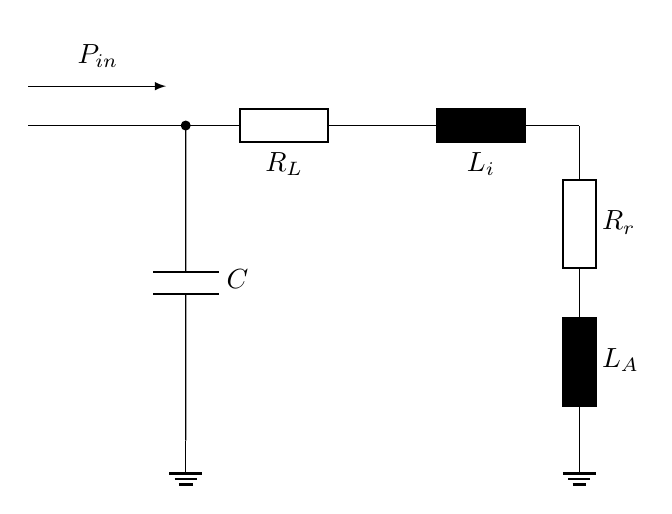
\begin{tikzpicture}
		% Paths, nodes and wires:
		\draw (11.75, 6) to[european inductor, l={$L_{i}$}] (9.75, 6);
		\draw (12, 2) to[european inductor, l_={$L_{A}$}] (12, 4);
		\draw (7, 6) to[capacitor, l={$C$}] (7, 2);
		\draw (12, 5.75) to[european resistor, l={$R_{r}$}] (12, 3.75);
		\draw (9.25, 6) to[european resistor, l={$R_{L}$}] (7.25, 6);
		\node[ground] at (7, 2){};
		\node[ground] at (12, 2){};
		\draw (7, 6) -- (5, 6);
		\node[circ] at (7, 6){};
		\draw (7, 6) -- (7.25, 6);
		\draw (9.25, 6) -- (10, 6);
		\draw (11.75, 6) -- (12, 6);
		\draw (12, 5.75) -| (12, 6);
		\draw[-latex] (5, 6.5) -- (6.75, 6.5);
		\node[shape=rectangle, minimum width=2.215cm, minimum height=0.965cm] at (6.534, 6.75){} node[anchor=north west, align=left, text width=1.827cm, inner sep=6pt] at (5.409, 7.25){$P_{in}$};
	\end{tikzpicture}
}
\caption{Full equivalent circuit}
\label{fig:eqc_balanis}

	\end{subfigure}
	\hfill
	\hspace*{-0.5cm}
	\begin{subfigure}[b]{0.45\textwidth}
	\centering
	\resizebox{0.65\textwidth}{!}{
	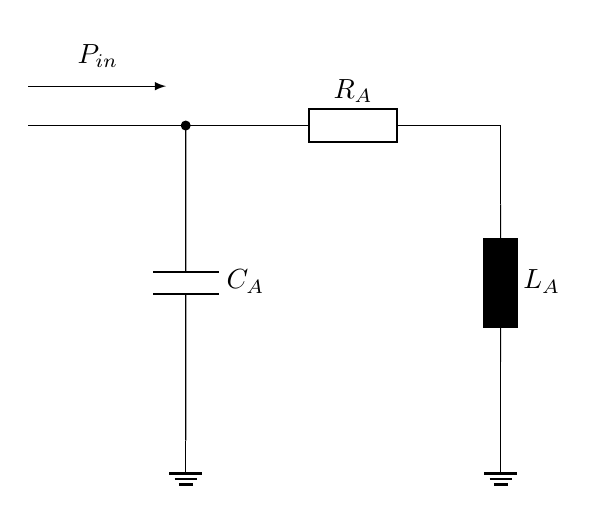
\begin{tikzpicture}
		% Paths, nodes and wires:
		\draw (11, 3) to[european inductor, l_={$L_{A}$}] (11, 5);
		\draw (7, 6) to[capacitor, l={$C_A$}] (7, 2);
		\node[ground] at (7, 2){};
		\node[ground] at (11, 2){};
		\draw (7, 6) -- (5, 6);
		\node[circ] at (7, 6){};
		\draw (7, 6) -- (7.25, 6);
		\draw[-latex] (5, 6.5) -- (6.75, 6.5);
		\node[shape=rectangle, minimum width=2.215cm, minimum height=0.965cm] at (6.534, 6.75){} node[anchor=north west, align=left, text width=1.827cm, inner sep=6pt] at (5.409, 7.25){$P_{in}$};
		\draw (11, 2) -| (11, 3);
		\draw (7.25, 6) to[european resistor, l={$R_A$}] (11, 6);
		\draw (11, 6) -- (11, 5);
	\end{tikzpicture}
}
\caption{Reduced equivalent circuit}
\label{fig:eqc_simple}
	\end{subfigure}
	
	\caption{A full equivalent circuit of the small loop antenna, and a simplified version of it}
	\label{fig:eqc_loop}
\end{figure}


\begin{figure}[htbp]
	\centering
	\resizebox{\textwidth}{!}{%
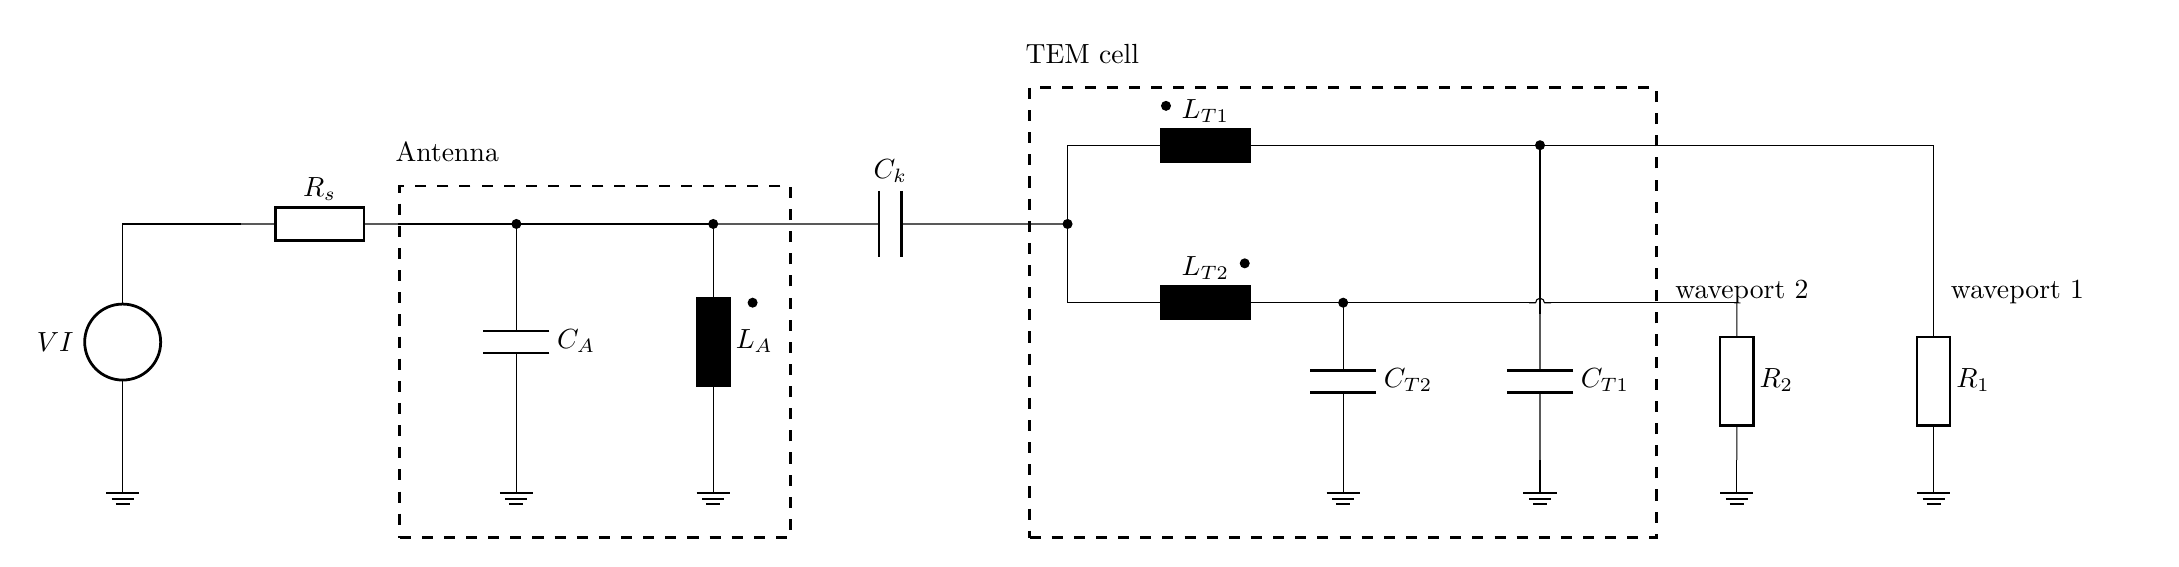
\begin{tikzpicture}
	% Paths, nodes and wires:
	\node[shape=circle, draw, line width=1pt, minimum width=0.965cm](N1) at (2.5, 9.5){} node[anchor=east] at (N1.west){$VI$};
	\node[ground] at (2.5, 8){};
	\draw (2.5, 9) -| (2.5, 8);
	\draw (4, 11) to[european resistor, l={$R_s$}] (6, 11);
	\draw (7.5, 11) to[capacitor, l={$C_A$}] (7.5, 8);
	\draw (10, 11) to[european inductor, l={$L_A$}] (10, 8);
	\node[ground] at (7.5, 8){};
	\node[ground] at (10, 8){};
	\draw (2.5, 10) -| (2.5, 11) -- (4, 11);
	\draw (6, 11) -- (7.5, 11) -- (10, 11);
	\node[circ] at (7.5, 11){};
	\node[circ] at (10.5, 10){};
	\node[shape=rectangle, draw, line width=1pt, dash pattern={on 4pt off 4pt}, minimum width=4.965cm, minimum height=4.465cm] at (8.5, 9.25){};
	\node[shape=rectangle, minimum width=5.215cm, minimum height=1.465cm] at (8.375, 11.5){} node[anchor=north west, align=left, text width=4.827cm, inner sep=6pt] at (5.75, 12.25){Antenna};
	\draw (10, 11) to[capacitor, l={$C_k$}] (14.5, 11);
	\node[circ] at (10, 11){};
	\draw (14.5, 10) to[european inductor, l={$L_{T2}$}] (18, 10);
	\draw (14.5, 12) to[european inductor, l={$L_{T1}$}] (18, 12);
	\draw (14.5, 10) -| (14.5, 12);
	\node[circ] at (14.5, 11){};
	\draw (18, 10) to[capacitor, l={$C_{T2}$}] (18, 8);
	\draw (23, 10) to[european resistor, l={$R_2$}] (23, 8);
	\node[ground] at (18, 8){};
	\node[ground] at (20.5, 8){};
	\node[circ] at (18, 10){};
	\draw (18, 12) -- (22, 12);
	\draw (20.5, 10) to[capacitor, l={$C_{T1}$}] (20.5, 8);
	\node[ground] at (23, 8){};
	\draw (25.5, 10) to[european resistor, l={$R_1$}] (25.5, 8);
	\node[ground] at (25.5, 8){};
	\draw (22, 12) -- (24.5, 12);
	\draw (20.5, 10) -- (20.5, 12);
	\node[jump crossing] at (20.5, 10){};
	\draw (18, 10) -- (20.36, 10);
	\draw (20.64, 10) -- (23, 10);
	\draw (24.5, 12) -| (25.5, 10);
	\node[circ] at (20.5, 12){};
	\node[shape=rectangle, draw, line width=1pt, dash pattern={on 4pt off 4pt}, minimum width=7.965cm, minimum height=5.715cm] at (18, 9.875){};
	\node[shape=rectangle, minimum width=5.215cm, minimum height=1.465cm] at (16.375, 12.75){} node[anchor=north west, align=left, text width=4.827cm, inner sep=6pt] at (13.75, 13.5){TEM cell};
	\node[shape=rectangle, minimum width=2.715cm, minimum height=0.965cm] at (23.375, 10){} node[anchor=north west, align=left, text width=2.327cm, inner sep=6pt] at (22, 10.5){waveport 2};
	\node[shape=rectangle, minimum width=2.715cm, minimum height=0.965cm] at (26.875, 10){} node[anchor=north west, align=left, text width=2.327cm, inner sep=6pt] at (25.5, 10.5){waveport 1};
	\node[circ] at (15.75, 12.5){};
	\node[circ] at (16.75, 10.5){};
\end{tikzpicture}
}
\caption{Circuit with voltage source, resistor, and capacitor.}
\label{fig:simple-circuit}
\end{figure}

The inductance and reactance is derived out of the parallel replacement circuit through 

\begin{subequations}
	\begin{equation}
	L = \frac{V^2}{2\omega^2W_m},
	\end{equation}
 	\begin{equation}
 	C = \frac{2W_c}{V^2}.
 	\end{equation}
\end{subequations}

Inserting the reactance values yield a good approximation of the real dipole moments. The behavior of the dipole moments can therefore be explained by the dominating inductance, which generates a large voltage, thus increasing the electric coupling. 

A fine mesh is important due to the near-fields of the antenna. Coarse meshes lead to bad modeling the the fields near the antenna, leading to bad current and voltage calculations in the antenna. A large part of this happens due to bad modeling of the displacement current near the port. Especially small values which are important, such as the capicitance responsible for electric coupling of the antenna, heavily suffer from the numerical error.

%\begin{figure}[htbp]
%	\centering
%	\begin{subfigure}[b]{0.48\textwidth}
%	\centering
%\includegraphics[width=1\linewidth]{content/img/loop_inductance}
%\caption{}
%\label{fig:loopinductance}
%	\end{subfigure}
%	\hfill
%	\begin{subfigure}[b]{0.48\textwidth}
%	\centering
%	\includegraphics[width=1\linewidth]{content/img/loop_capacitance}
%	\caption{}
%	\label{fig:loopcapacitance}
%	\end{subfigure}
%	
%	\caption{Dipole moments and phase shift of loop antenna}
%	\label{fig:example}
%\end{figure}

The capacitance of the antenna in the TEM cell is $C_{AT}=6.74\,\mathrm{pF}$ and the inductance $L_{AT}=16.51\,\mathrm{nH}$, approximately constant over frequency. In free space, the antenna has much lower inductance and capacitance values, which vary with frequency. \todo{plot free space capacitance and inductance values}

\todo{Replace all plots here. Use this ansys hfss solution setup as standard for all antennas and simulations}




\autoref{fig:dipole_moments_loop_antenna} shows the dipole moments of the loop antenna over frequency. As expected, the magnetic dipole moment $m_\mathrm{m}$ contributed the largest amount to the antenna coupling. A small amount of electric dipole moment is also present, which naturally occurs due to the current wire aligned with the TEM electric fields. The electric dipole moment $m_\mathrm{e}$ increases non-linearly with frequency. The calculations with the S-parameters proved to have lower numerical deviations than other methods, such as integrating fields in the antenna region. Those results showed to fluctuate heavily, likely due to low resolution around the small antenna region, leading to larger errors. Calculating with S-parameters bypasses this problem.

\begin{figure}[h]
	\centering
	\includegraphics[width=0.7\linewidth]{content/img/curr_imp}
	\caption{Magnitude and phase of the impedance of the current loop antenna.}
	\label{fig:currimp}
\end{figure}

The impedance was calculated by dividing the voltage and current at the feedpoint. However, due to the phase being small in value and prone to numerical errors, it has been determined by evaluating the complex power $S$ and then the imaginary power $Q$ through

\begin{equation}
	Q = \sqrt{S^2 - P^2}
\end{equation}

The real power consumed at the antenna input is roughly equal to the real power at one waveport. This is due to the almost 180° phase shift between the power at output ports, which does not require the antenna to provide the real power for both ports at once.

\subsubsection{Current distribution on septum}

\begin{figure}[h]
	\centering
	\includegraphics[width=1\linewidth]{content/img/loop_surface_currents.png}
	\caption{Surface current density of septum induced by loop antenna at 3\,GHz}
	\label{fig:current_loop_surface_current}
\end{figure}

\todo[inline]{change jsurf name in legend to something different}


Note that the surface current density in \autoref{fig:current_loop_surface_current} is much more concentrated in the center. In the case of the monopole antenna, the current density distributed almost equally around the septum. In the case of the loop antenna, the current below the antenna seems to be cut off by the rotational eddy currents next to them. Furthermore, the phase shift between the currents at the output ports is 180°, leading to the perceived phase shift of magnetic dipole moments.

\autoref{fig:current_loop_surface_current_offset} demonstrates the surface current density when shifting the loop antenna 7.5\,cm (quarter of the septum width) in y-direction. The coupling and transferred energy remains roughly the same.

\begin{figure}[h]
	\centering
	\includegraphics[width=1\linewidth]{content/img/current_loop_surface_current_offset.png}
	\caption{Surface current density at 550\,MHz with offset}
	\label{fig:current_loop_surface_current_offset}
\end{figure}

\autoref{fig:current_loop_surface_current_rotated} shows the surface current density when rotating the antenna by 90°. Only a negligible amount reaches the output ports, leading to no coupling.  

\begin{figure}[h]
	\centering
	\includegraphics[width=1\linewidth]{content/img/current_loop_surface_current_rotated.png}
	\caption{Surface current density at 550\,MHz with rotated antenna}
	\label{fig:current_loop_surface_current_rotated}
\end{figure}

\autoref{fig:current_loop_surface_current_offset_rotated} shows the current distribution of the current loop antenna, when it is rotated and contains an offset. Again, the eddy currents dominate. However, some of those currents propagate towards the output ports, increasing the energy transfer minimally (0.5\,dB). Additionally, the energy transferred is in phase, which makes it indistinguishable from an electric dipole.

\begin{figure}[h]
	\centering
	\includegraphics[width=1\linewidth]{content/img/current_loop_surface_current_offset_rotated.png}
	\caption{Surface current density at 550\,MHz with offset and rotated antenna}
	\label{fig:current_loop_surface_current_offset_rotated}
\end{figure}

\todo{annotate maximum and minimum current densities}



\autoref{fig:currentloopchargedistribution} shows the charge density distribution in the current loop antenna. Charges collect, among other locations, at the bottom wire. This leads to electric coupling with the septum. 

\begin{figure}[htbp]
	\centering
	\begin{minipage}[b]{0.45\textwidth}
		\centering
		\includegraphics[width=0.5\linewidth]{content/img/current_loop_charge_distribution}
		\caption{Charge density distribution in current loop antenna}
		\label{fig:currentloopchargedistribution}
	\end{minipage}
	\hfill
	\begin{minipage}[b]{0.45\textwidth}
		\centering
		\includegraphics[width=0.5\linewidth]{content/img/current_loop_current_distribution}
		\caption{Current density distribution in current loop antenna}
		\label{fig:currentloopcurrentdistribution}
	\end{minipage}
\end{figure}


The current and voltage drops along the wire are not constant. From the feedpoint to the first corner, there is a much larger voltage drop and current, than from the second corner to the ground plane. Consequently, the power consumed by the first part is much higher than by the latter \todo{Insert power consumption plots of each antenna section}. Additionally, this difference in power consumption increases slightly over frequency. 

The electric current reduces over the wire because of the displacement current to the septum and the ground plane. As visible in the charge density plot in \autoref{fig:currentloopcurrentdistribution} and the electric field plot in \autoref{fig:currentloopnearefield}, much of the displacement current occurs near the feedpoint and at the wire parallel to the septum. Consequently, this is where the current drops by the most amount. \todo{Insert current distribution plots}



\begin{figure}[htbp]
	\centering
	\begin{minipage}[b]{0.45\textwidth}
		\centering
		\includegraphics[width=0.7\linewidth]{content/img/current_loop_near_e_field}
		\caption{Electric near field in current loop antenna}
		\label{fig:currentloopnearefield}
	\end{minipage}
	\hfill
	\begin{minipage}[b]{0.45\textwidth}
		\centering
		\includegraphics[width=0.7\linewidth]{content/img/current_loop_near_h_field}
		\caption{Magnetic near field in current loop antenna}
		\label{fig:currentloopnearhfield}
	\end{minipage}
\end{figure}


\todo{H-field from other perspective?}



\autoref{fig:currentloopfeedcurrent} and \autoref{fig:currentloopvoltagedrop} show the current and voltage consumption of the antenna. The phase shift equals $\phi\approx89.80\circ$, which hints to a strong inductive behavior. The inductance is determined to be $L\approx2.15\,\mathrm{nH}$. The capacitance is very low, but does lead so some displacement current. The frequency behavior of the voltage and current interchange if the antenna is strongly capacitive, as it the case in a monopole antenna.

A theoretical approach to approximate the inductance of a current loop in free-space is \cite[p. 245]{Balanis_1997}

\begin{equation}
	L_A = \frac{2\mu_0 a}{\pi} \left[ \ln\!\left(\frac{a}{b}\right) - 0.774 \right],
\end{equation}

which yields $L=2.32\,\mathrm{nH}$. However, this does not consider the coupling effects of the TEM cell.


Next, the electric and magnetic near field is investigated. The wave impedance $Z=E/H$ shown in \autoref{fig:waveimpedanceloop} in the center of the loop rises linearly over frequency. At low frequencies, the wave impedance is very low, which confirms the inductive behavior of the antenna. However, as the frequency increases, so does the voltage drop. This may be analogous to a inductor in an electrical circuit, across which the voltage drop also increases with frequency $U = \mathrm{i}L\omega I$. 


\autoref{eqn:a_b_moments_simp} relates the dipole moments to the output power. The influence of the dipole moments is determined by the electric field at the electric dipole moment and the magnetic field at the magnetic dipole moment. In this formula, the electric and magnetic field are simply related through the free-space wave impedance. However, as visible in \autoref{fig:waveimpedanceloop}, the wave impedance at the location of the dipole moments (i.e. at the antenna) is much lower. Additionally, it rises linearly with the frequency. This influence of the antenna itself on the fields around the dipoles could explain the non-linear relation of the dipole moments to the frequency.



\autoref{fig:currentlooppowerconsumption} shows the power consumption of the antenna, which is influenced by two factors. The radiation resistance rises quadratically with the frequency. At the same time, the impedance increases, leading to higher matching and therefore to a higher power transfer. This is contrary to the monopole antenna, where the impedance is decreases over the frequency, again leading to better impedance matching, because the impedance was high to begin with. The source impedance is 50\,$\Omega$.

\autoref{fig:deleteafter} shows the total power maintained in the system, meaning $S_{11}^2+S_{12}^2+S_{13}^2$. It does not add up to one, meaning that some energy is lost due to finite conductivity of the septum and antenna. This energy dispersion increases with frequency, most likely due to a decrease of the conductivity due to high-frequency effects like the Skin-effect. Consequently, the power consumption in \autoref{fig:currentlooppowerconsumption} shows a square root relation to the frequency, because the power dispersion is so high. When changing the material of the antenna and septum to a perfect electric conductor, the total power in a system remains one (no power is dispersed) and the power consumption over frequency of the antenna shows a quadratic relation to the frequency, due to the quadratic increase of the radiation resistance.


The Skin-effect reduces the area in which the current flows, therefore increasing resistance. This appears due to the reduction of the depth, in which the electromagnetic waves enter. It is also called Skin depth and mathematically described by \autoref{eqn:skin_depth}. It depends on the imaginary part of the wave number $\kappa$, which is described in \autoref{eqn:kappa}. For high conducting materials $\left(\sigma >> \epsilon\omega\right)$, the dependency of the skin depth $d$ on the frequency can be described therefore as $d \propto 1/\sqrt{\omega}$. Since the power dispersion is linearly proportional to the area of the conductor and therefore Skin-depth, it shows the same dependency on the frequency $P_\mathrm{disp}\propto 1/\sqrt{\omega}$ \cite{Griffiths_2024}.  
\todo{Own little chapter for skin effect? Loop antennas are known for higher conductor losses than radiation Balanis page 231}

\begin{subequations}
	\begin{equation}
		\kappa = \omega \sqrt{\frac{\epsilon \mu}{2}}\left[\sqrt{ 1+\left(\frac{\sigma}{\epsilon\omega}\right) ^2 } -1\right]^{1/2}
		\label{eqn:kappa}
	\end{equation}
	\begin{equation}
		d = 1/\kappa
		\label{eqn:skin_depth}
	\end{equation}
\end{subequations}

At 1\,GHz, the dispersed power already equals to 0.46\,\%, which is much higher than the power transfer of the antenna to one waveport of 1.26e-5 at that frequency. Because this dispersed power is proportional to the square-root of the frequency $P_\mathrm{disp}\propto 1/\sqrt{\omega}$, the overall transferred power to the antenna shows the same characteristic. However, the power transfer to the waveports has a quadratic dependency on the frequency. %This, in turn, also leads to the unusual relation of the electric dipole moment to the frequency. 
\todo{explain better.}

This dispersed power may be ignored in the simulations by changing the antenna's material (main source of power dissipation) and the septum from copper to a perfect electric conductor. The overall power in the system then remains at a constant one over the whole frequency range. Additionally, the transferred power to the antenna now has a quadratic relationship with the frequency, indicating increased radiation efficiency, previously described by \autoref{eqn:elec_rad_res}. 
\todo{Show plots?}

\begin{figure}[htbp]
	\centering
	\begin{subfigure}[b]{0.48\textwidth}
		\centering
		\includegraphics[width=1\linewidth]{content/img/loop_opower}
		\caption{}
		\label{fig:loopopower}
	\end{subfigure}
	\hfill
	\begin{subfigure}[b]{0.48\textwidth}
		\centering
		\includegraphics[width=1\linewidth]{content/img/loop_opower_comp}
		\caption{}
		\label{fig:loopopowercomp}
	\end{subfigure}
	
	\caption{Dipole moments and phase shift of loop antenna}
	\label{fig:example}
\end{figure}

Possible reasons for the deviation in power are numerical inaccuracies or the coupling of the TE\textsubscript{01} mode, which changes the field distribution in a disadvantageous way.

The current-loop antenna contains two electric dipoles, shifted in phase by 180°. They therefore oppose each other in the power transfer to the waveports. However, as visible in the electric near field plot in \autoref{fig:currentloopvoltagedrop}, the electric dipole moment from node A to the feedpoint is much larger than the one from node B to ground. The reason can be demonstrated by representing the antenna with its nodes in \autoref{fig:current_loop_ua_ub}. The partial inductances in this schematic are much larger than the capacitances. This leads to a large voltage drop between node A and B, and therefore a weaker electric dipole moment at node B.

Additionally, this voltage difference $V_\mathrm{A}-V_\mathrm{B}$ rises linearly over the frequency, due to the linearly increasing impedance of the inductance $\mathrm{i}\omega L$. This means, that the over electric dipole moment a quadratic relationship to the frequency has.
\todo{Magnetic moment equivalent antenna. Explain with current and H-field, too}

\todo{Prove square frequency dependency}

Further, \autoref{fig:loopwaveimp} shows the wave impedance of the near-fields at the loop antenna. The \autoref{eqn:a_b_moments_simp} shows, that the influence of the dipoles depends on the electric and magnetic fields at the dipoles position. The electric and magnetic fields are related through the wave impedance $Z = E/H$. If the wave impedance rises linearly over frequency, the electric field increases over the magnetic fields, giving more influence to the electric dipole moments. As previously discussed, there are two electric dipole moments in this antenna, benefiting from that. \todo{Monopole antenna: Also change in wave impedance, but there is not really a magnetic dipole moment} 



The wave impedance $Z_\mathrm{w}$ in the near field of the electrically small loop antenna is approximated by \autoref{eqn:wave_impedance_loop}. It confirms the linear relationship of the near-field wave impedance to the frequency. \todo{Source: \href{https://en.wikipedia.org/wiki/Near_and_far_field}{Wikipedia}. I couldn't find the source in the reference books. TODO}


\begin{equation}
	\left|Z_\mathrm{w}\right|\approx 2 \pi^2 \cdot 240\,\Omega \cdot\frac{r\cdot f}{c}
	\label{eqn:wave_impedance_loop}
\end{equation}


\FloatBarrier

\subsubsection{Loop antenna with gap}\label{sec:loop_gap_sim}
\begin{figure}[h]
	\centering
	\includegraphics[width=0.5\linewidth]{content/img/gapped_loop_antenna}
	\caption{Geometry of loop antenna with a gap in the return path inserted into the TEM cell.}
	\label{fig:gappedloopantenna}
\end{figure}

The loop is not closed, therefore, a simple calculation of the magnetic flux is not possible. Instead, the closed field integral of the electric field can be evaluated, where the integral of the gap region is set to zero. An equivalent electric field can be found, with which a magnetic field is easy to find. 

\begin{figure}[htbp]
	\centering
	\begin{subfigure}[b]{0.48\textwidth}
	\centering
\includegraphics[width=1\linewidth]{content/img/gapped_loop_moments}
\caption{}
\label{fig:gappedloopmoments}
	\end{subfigure}
	\hfill
	\begin{subfigure}[b]{0.48\textwidth}
	\centering
\includegraphics[width=1\linewidth]{content/img/gapped_loop_phase}
\caption{}
\label{fig:gappedloopphase}
	\end{subfigure}
	
	\caption{Dipole moments and phase shift of loop antenna}
	\label{fig:example}
\end{figure}


\begin{figure}[htbp]
	\centering
	\begin{subfigure}[b]{0.48\textwidth}
	\centering
\includegraphics[width=1\linewidth]{content/img/gapped_loop_opower}
\caption{}
\label{fig:gappedloopopower}
	\end{subfigure}
	\hfill
	\begin{subfigure}[b]{0.48\textwidth}
	\centering
\includegraphics[width=1\linewidth]{content/img/gapped_loop_voltage}
\caption{}
\label{fig:gappedloopvoltage}
	\end{subfigure}
	
	\caption{Dipole moments and phase shift of loop antenna}
	\label{fig:example}
\end{figure}



\begin{figure}[htbp]
	\centering
	\begin{subfigure}[b]{0.48\textwidth}
	\centering
\includegraphics[width=1\linewidth]{content/img/gapped_loop_current}
\caption{}
\label{fig:gappedloopcurrent}
	\end{subfigure}
	\hfill
	\begin{subfigure}[b]{0.48\textwidth}
	\centering
\includegraphics[width=1\linewidth]{content/img/gapped_loop_imp}
\caption{}
\label{fig:gappedloopimp}
	\end{subfigure}
	
	\caption{Dipole moments and phase shift of loop antenna}
	\label{fig:example}
\end{figure}



\FloatBarrier

\subsubsection{Inverted F-antenna}\label{sec:ifa_sim}

The inverted F-antenna (IFA) is modeled in Ansys HFSS as shown in \autoref{fig:ifa}. It is positioned at the center of the TEM cell, mounted at the top surface. The 5\,mm long wire points towards waveport 2. The excitation is a modal wave port. With a maximum dimension of 5\,mm, the antenna is electrically small for a frequency of up to 6\,GHz, at which it will be a tenth of the wavelength. In this simulation, the antenna is investigated for the frequency of 100\,MHz to 1\,GHz. The TEM cell has a width of 40\,mm and a height of 24\,mm and an impedance of $\sim50\,\Omega$. The goal is to find equivalent dipole moments of the antenna. 


\begin{figure}[h]
	\centering
	\includegraphics[width=0.75\linewidth]{content/img/inverted_f_antenna.png}
	\caption{Inverted F-antenna used in the simulation}
	\label{fig:ifa}
\end{figure}




\begin{figure}[htbp]
	\centering
	\begin{subfigure}[b]{0.48\textwidth}
	\centering
\includegraphics[width=1\linewidth]{content/img/inverted_f_dipoles}
\caption{Dipole moments}
\label{fig:invertedfdipoles}
	\end{subfigure}
	\hfill
	\begin{subfigure}[b]{0.48\textwidth}
	\centering
\includegraphics[width=0.95\linewidth]{content/img/inverted_f_dipoles_phase}
\caption{Phase}
\label{fig:invertedfdipolesphase}
	\end{subfigure}
	
	\caption{Dipole moments and phase shift of loop antenna}
	\label{fig:example}
\end{figure}

\begin{figure}[h]
	\centering
	\includegraphics[width=0.7\linewidth]{content/img/inverted_f_opower}
	\caption{Output power and electric field at output.}
	\label{fig:invertedfopower}
\end{figure}


\begin{figure}[htbp]
	\centering
	\begin{subfigure}[b]{0.48\textwidth}
	\centering
\includegraphics[width=1\linewidth]{content/img/inverted_f_current}
\caption{Current}
\label{fig:invertedfcurrent}
	\end{subfigure}
	\hfill
	\begin{subfigure}[b]{0.48\textwidth}
	\centering
\includegraphics[width=1\linewidth]{content/img/inverted_f_voltage}
\caption{Voltage}
\label{fig:invertedfvoltage}
	\end{subfigure}
	
	\caption{Voltage and current at feedpoint of inverted-F antenna.}
	\label{fig:example}
\end{figure}

\begin{figure}[h]
	\centering
	\includegraphics[width=0.7\linewidth]{content/img/inverted_f_impedance}
	\caption{Phase and magnitude of the inverted-F antenna's impedance over frequency.}
	\label{fig:invertedfimpedance}
\end{figure}




\autoref{fig:dipole_moments_over_freq_ifa} shows the dipole moments over frequency. The electric dipole moment $m_e$ has been normalized to the free-space wave impedance of $377\,\Omega$ to make the dipole moments comparable. This is possible because the dipole moments are interchangeable through the wave impedance \cite[p. 414]{Jackson}. The antenna input power has been set to 142588.47\,W, because this leads to an output power of 1\,W at a frequency of 1\,GHz. The magnetic dipole moment is much larger than the electric dipole moment, because the current loop of the antenna is aligned with the TEM cell's magnetic fields, but the line current is not with the TEM electric fields. The magnetic dipole moments rises linearly with the frequency, which is equal to a quadratic increase of power. Only the TEM modes has been considered in the simulation, as other modes disturb the calculations. 



\todo{Repeat for different orientations? Change variable name: TEM cell height.}

The magnetic coupling with the septum happens due to the alignment of the current loop with the magnetic field of the dominant TEM mode. The antenna is now rotated by 90° around the z-axis, such that the magnetic current loop stands perpendicular to the magnetic TEM fields. \autoref{fig:phase_shift_90_ifa} demonstrates the phase of the S-parameters, describing the coupling of antenna to waveport 1 and 2. Since the magnetic dipole moment is responsible for a phase between the ports, \autoref{fig:phase_shift_90_ifa} strongly hints to an absence of it.


\autoref{dipole_moments_ifa_90} shows that the electric dipole moment $m_\mathrm{e}$ has stayed the same, while the magnetic dipole moment became zero. Consequently, the overall power transfer between the antenna and the waveports is also much lower. 

\todo{The same procedure was repeated with different dipole moments positions, for which \autoref{eqn:e0z_mse} worked. Maybe do a general equation for the normalized e-field?}


\FloatBarrier
\subsubsection{Center Fed Monopole Antenna}

The center fed monopole antenna is shown in \autoref{fig:center_fed_monopole}. The conducting plane in \autoref{fig:center_fed_monopole} is on the top side of the TEM cell, thus the image is rotated counter-clockwise by 90 degrees. The electric wire with the length of 5 mm points towards the septum. The 1.1 x 1.6 mm loop is again aligned with the magnetic field lines of the TEM mode. The antenna is fed with a power of $P_\mathrm{Antenna}=127770.39\,\mathrm{W}$, which once more leads to an output power of $P_\mathrm{Out}=1\,\mathrm{W}$ at 1\,GHz at both output ports. 

\begin{figure}[h]
	\centering
	\includegraphics[width=0.3\linewidth]{content/img/center_fed_monopole.png}
	\caption{Center fed monopole antenna used in simulation}
	\label{fig:center_fed_monopole}
\end{figure}

The magnitude of $|S_\mathrm{A1}|=|S_\mathrm{A2}|$ in \autoref{fig:forward_coeff_cfm} shows stronger coupling. As will be seen below, this is because of an increased electric dipole moment, while the magnetic dipole moment remained the same. Therefore, the center fed monopole antenna couples well electrically with the TEM cell.

\begin{figure}[h]
	\centering
	\includegraphics[width=1\linewidth]{content/img/forward_coeff_cfm.png}
	\caption{S-parameter describing coupling of antenna to waveport 1}
	\label{fig:forward_coeff_cfm}
\end{figure}

\begin{figure}[htbp]
	\centering
	\begin{minipage}[t]{0.48\textwidth}
		\centering
		\includegraphics[width=0.85\linewidth]{content/img/phase_shift_cfm.png}
		\caption{Phase shift}
		\label{fig:phase_shift_cfm}
	\end{minipage}
	\hfill
	\begin{minipage}[t]{0.48\textwidth}
		\centering
		\includegraphics[width=1\linewidth]{content/img/dipole_moment_cfm.png}
		\caption{Dipole moments}
		\label{fig:dipole_moment_cfm}
	\end{minipage}
\end{figure}



\begin{figure}[htbp]
	\centering
	\begin{minipage}[b]{0.45\textwidth}
	\centering
\includegraphics[width=1\linewidth]{content/img/cfm_opower}
\caption{Output power and electric field of center-fed monopole antenna}
\label{fig:cfmopower}
	\end{minipage}
	\hfill
	\begin{minipage}[b]{0.45\textwidth}
	\centering
\includegraphics[width=1\linewidth]{content/img/cfm_imp}
\caption{Magnitude and phase of center-fed monopole antenna's impedance.}
\label{fig:cfmimp}
	\end{minipage}
\end{figure}


\autoref{fig:dipole_moment_cfm} shows that the magnetic dipole moments of the inverted F and center fed monopole antennas are equal. This is due to the same size of the current loops. However, the electric dipole moments increased for the center fed monopole antenna. The alignment of the line current with the TEM cell's electric field causes this. (antenna power = 126549.7191667088\,W)


\begin{figure}[htbp]
	\centering
	\begin{subfigure}[b]{0.48\textwidth}
		\centering
		\includegraphics[width=1\linewidth]{content/img/cfm_voltage}
		\caption{Voltage}
		\label{fig:cfmvoltage}
	\end{subfigure}
	\hfill
	\begin{subfigure}[b]{0.48\textwidth}
		\centering
		\includegraphics[width=1\linewidth]{content/img/cfm_current}
		\caption{Current}
		\label{fig:cfmcurrent}
	\end{subfigure}
	
	\caption{Voltage and current at feedpoint of center-fed monopole antenna.}
	\label{fig:example}
\end{figure}




The output power has been scaled as in the simulation before. This leads to the same electric field magnitude. Therefore, the electric field and output power over frequency plot are the same as in the case for the inverted F antenna, visible in \autoref{fig:output_power_e_fields_over_freq_ifa}.


When rotating this antenna by 79°, the electric and magnetic dipole moment influence the output power by roughly the same amount, as visible in \autoref{fig:79cfm}. This makes itself manifest by a phase shift of around 45°  between the output powers of the waveports. Interestingly, both the electric and the magnetic dipole moment demonstrate a non-linear behavior. \todo{Why does the magnetic moment sink?}

\todo{CFM at 90° rotation still demonstrates magnetic dipole moment, opposed to current loop. Does this scale with antenna height, i.e. electric dipole moment?}

\FloatBarrier



\subsubsection{Serial Loop Antenna}

This section will discuss the antenna displayed in \autoref{fig:serialloopantenna}. The idea of that antenna is to create two magnetic dipole moments, which are in phase. As the frequency increases, the displacement current between the loops becomes larger, thus reducing the current through and weakening the second loop. The dipole moments in \autoref{fig:serialloopantennadipolemoments} demonstrate a non-linear behavior of the magnetic dipole moment (only very weakly recognizable, but with a geometry sweep this becomes clearer \todo{Find a geometry where this effect is much stronger}). Also, it would be interesting to measure the wave impedances in both loops over the frequency. Also, find the current distributions, add current plots and electric fields, charge distributions.  

\begin{figure}[h]
	\centering
	\includegraphics[width=0.3\linewidth]{content/img/serial_loop_antenna}
	\caption{Serial loop antenna}
	\label{fig:serialloopantenna}
\end{figure}
\begin{figure}[h]
	\centering
	\includegraphics[width=1\linewidth]{content/img/serial_loop_antenna_dipole_moments}
	\caption{Dipole moments }
	\label{fig:serialloopantennadipolemoments}
\end{figure}

\FloatBarrier

\subsubsection{Offset of source antennas and eddy currents}

\todo{Relate the offset to the normalized E field distribution. For Example, the vertical part of the current loop antenna does not influence the TEM cell coupling without offset, which can be shown with the normalized E field distribution.}

\todo{Can the normalized h-field distribution be related to the E field by multiplying it with the free-space wave impedance? How does a 90° rotated current loop antenna couple with offset? There should be some coupling due to the existence of normalized h-fields there}

\colorbox{red}{This section is probably wrong.}

Next, the CFM is rotated by an angle. This angle is swept from 0° to 90°, iteratively increased by 1° [deg]. At 90° the magnetic dipole moment is at a minimum, while it is the largest at 0°. The idea is now to find a balance between the electric and magnetic dipole moment, such that the antenna operates in a way of resonance. In this operation, the S11 parameter shall be the lowest, even though the coupling of the magnetic field only becomes weaker with increasing angle \todo{Is it possible to proof this by mathematics?}. The reason for this approach by increasing angle is that it is otherwise very hard to achieve such a balance between the dipole moments by purely scaling the antenna. The electric dipole moment is very weak, and when increasing the antenna height (thus only the electric dipole moment), it soon becomes very large and even touches the septum. Rotating the angle instead becomes a very efficient alkternative. This has been determined just by looking at the phase shifts from the antenna to the waveports: If electric and magnetic dipole moments are roughly equally influential, then the phase shift between the ports shall be 90°\todo{Show mathematically?}. Very important for these simulation is the renormalization of the waveports \todo{Describe this in HFSS section, under excitations}. This enables the port exciting the antenna to have an impedance of 50 Ohm, independent of size. This will make a geometry sweep of the antenna able, without influencing the impedance of the port exciting the antenna (Imagine a coax cable attached to the antenna. It is hinted by the round waveport in the model. When it gets shifted around, its wave impedance changes, and so does the reflection, and the results are distorted) 




\FloatBarrier

\autoref{fig:cfm_rotation_sweep} it is visible, that the lowest S11 (least reflections) is achieved at a rotation angle of 72°. \todo{Why, how do the dipole moments look like there? Anf is this just a numerical error?}

\begin{figure}[h]
	\centering
	\includegraphics[width=1\linewidth]{content/img/cfm_rotation_sweep.png}
	\caption{CFM S11 sweep with rotation angle stepping}
	\label{fig:cfm_rotation_sweep}
\end{figure}


Eddy currents occur on the septum. They increase with frequency. When they get too large, the next-order mode starts propagating. Offsetting the antenna / dipole moment in y-direction reduces the amount of influence of the eddy current on the power carrying current in the septum. 

\todo{How does offset influence the eddy currents and the result?}


When implementing an offset in the center fed monopole antenna, the coupling between the waveports and the antenna changes. The change is visible in \autoref{fig:DELETE_AFTER}, although the magnitude of the coupling to both ports is the same.

\todo{Better investigation of offset: Show coupling and eddy currents}

\begin{figure}[h]
	\centering
	\includegraphics[width=1\linewidth]{content/img/DELETE_AFTER.png}
	\caption{Center fed monopole antenna coupling dependence on offset (Delete after)}
	\label{fig:DELETE_AFTER}
\end{figure}


\subsection{Dipole Moments}


\FloatBarrier
\subsubsection{Orientation and position in TEM Cell}

\autoref{fig:eyezcouplingcomparison} demonstrates the normalized output power of an electric dipole moment pointing in y-direction, and one in z-direction. This simulation only demonstrates the coupling behavior of the dipole moments over frequency, to explain the non-linear coupling of certain antennas. If dipole moments in certain positions and orientations couple with a different proportionality than the standard two dipole moments (ez and my), then the non-linear coupling may be explained that way.

\begin{figure}[h]
	\centering
	\includegraphics[width=1\linewidth]{content/img/ey_ez_coupling_comparison}
	\caption{Comparison of normalized output power of electric dipole moments}
	\label{fig:eyezcouplingcomparison}
\end{figure}

The electric dipole moment in z-direction $e_\mathrm{z}$ demonstrates the expected behavior: As the frequency rises, this dipole moment rises linearly and thus increases the output power quadratically. The electric dipole moment in y-direction $e_\mathrm{y}$ also increases linearly increase with frequency, but does not significantly change the output power for the low frequencies. However, as the frequency approaches the cut-off frequency of the next-higher order mode, the coupling rises significantly.

This simulation is repeated where the dipole moments are located at a height of $h=6\,\mathrm{mm}$, which is the dead center of the TEM cell, and $h=9\,\mathrm{mm}$, which is near the top wall of the TEM cell. The simulation results are similar for both cases. 

Most importantly, this simulation shows that the dipole moments have a relation to the frequency independent on their position. While their magnitude themselves do depend on the position, the relation to the frequency does not. 

\todo{Repeat Simulation for several other dipole moment positions and orientations?} 

\FloatBarrier
\subsubsection{Combining dipole moments with antennas}

\FloatBarrier
\subsubsection{Application of dipole moments}
As show in the previous simulations, antennas may be represented by dipole moments. This can be done in simulation models, which would otherwise be computationally too effortful. The dipole moments may be put into a shielded enclosure around a larger electronic system, as has been done in \cite{10274360}.


\FloatBarrier

\subsection{Investigation of field regions}

\todo[inline]{Update field plots}

In this section, the influence of the field region described in \autoref{sec:rad_fields} on the dipole moments are investigated. Making the TEM cell larger, such that $k\cdot r > 1$, is hardly possible without enabling higher-order modes to propagate. On the other hand, making the TEM cell smaller such that $k\cdot r \ll 1$, proves to be feasible. The following simulations are conducted with a TEM cell of dimensions $a=10\,\mathrm{mm}$ and $b=6\,\mathrm{mm}$, visible in \autoref{fig:krtemcell}.  

\begin{figure}[h]
	\centering
	\includegraphics[width=0.7\linewidth]{content/img/kr_tem_cell}
	\caption{TEM cell containing dipole moments}
	\label{fig:krtemcell}
\end{figure}


First, the current loop antenna used in \autoref{sec:loop_sim} is placed in the dead center of the TEM cell. The equivalent dipole moments are shown in \autoref{fig:loop_small_tem_moments}. In the \autoref{fig:dipole_moments_loop_antenna_copy} next to it, the dipole moments of the same antenna in the larger TEM cell used before ($a=40\,\mathrm{mm}$ and $b=24\,\mathrm{mm}$) are presented. 

\todo{The e field approx. in the python code is based on the large TEM cell. Therefore, the magnitude of the dipole moments of the small TEM cell are probably off}
\begin{figure}[htbp]
	\centering
	\begin{minipage}[t]{0.48\textwidth}
	\centering
\includegraphics[width=1\linewidth]{content/img/loop_small_tem_moments.png}
\caption{Moments in small TEM cell}
\label{fig:loop_small_tem_moments}
	\end{minipage}
	\hfill
	\begin{minipage}[t]{0.48\textwidth}
	\centering
	\includegraphics[width=1\linewidth]{content/img/dipole_moments_loop_antenna.png}
	\caption{Moments in normal TEM cell}
	\label{fig:dipole_moments_loop_antenna_copy}
	\end{minipage}
\end{figure}

This is done to compare the dipole moments in both cases. While they clearly increased by magnitude in case of the small TEM cell due to better coupling, their non-linear frequency relation still remains. This means that the change of field regions is not the reason for this behavior.

\todo{Insert kr, describe where r is measured, describe why the suspicion was that kr could influence this and how the fields change in the regions as described in the theoretical parts. Insert small current loop simulation. Insert Dipole Moment Simulations}

The $k\cdot r$ factor is determined in \autoref{fig:kranalysissmalltem} in the frequency range from 1\,MHz to 3\,GHz for the small TEM cell. This factor does not surpass 0.1, thus fulfilling the requirement $k\cdot r \ll 1$ for this investigation. For comparison, the $k\cdot r$ factor over a wider frequency range are shown in \autoref{fig:kranalysissmalltem} for the normal sized TEM cell ($a = 40\,\mathrm{mm}$ and $b = 24\,\mathrm{mm}$) and a degenerately high TEM cell ($a = 10\,\mathrm{mm}$ and $b=44\,\mathrm{mm}$). The high TEM does not have a port impedance of $50\,\Omega$, and is an attempt to achieve a large $k\cdot r$ factor without higher-order modes propagating. The markers in \autoref{fig:kranalysis} indicate the cut-off frequency, in which the next higher-order mode propagates. They demonstrate, that even in the high TEM cell a $k\cdot r = 1$ is not achieved.


\begin{figure}[htbp]
	\centering
	\begin{minipage}[t]{0.48\textwidth}
	\centering
	\includegraphics[width=1\linewidth]{content/img/kr_analysis_small_TEM}
	\caption{$k\cdot r$ in small TEM cell}
	\label{fig:kranalysissmalltem}
	\end{minipage}
	\hfill
	\begin{minipage}[t]{0.48\textwidth}
	\centering
	\includegraphics[width=1\linewidth]{content/img/kr_analysis}
	\caption{$k\cdot r$ for other TEM cells}
	\label{fig:kranalysis}
	\end{minipage}
\end{figure}
\todo{Fix figures: Titles and Legends}

Now, three simulations are conducted with different excitation sources in the small TEM cell:

\begin{itemize}
	\item The current loop 
	\item The equivalent dipole sources $e_z$ and $m_m$ of the current loop
	\item The equivalent magnetic dipole source $m_m$, neglecting $e_z$
\end{itemize}

\autoref{fig:outputpowercomparisonsmalltem} shows the output power over frequency normalized to 1\,W for all three constellations. The normalization is done to qualitatively discuss the frequency-dependent coupling behavior. \autoref{fig:phaseshiftcomparisonsmalltem} demonstrates the phase shift between the powers at the two waveports over frequency.

\begin{figure}[htbp]
	\centering
	\begin{minipage}[t]{0.48\textwidth}
		\centering
		\includegraphics[width=1\linewidth]{content/img/output_power_comparison_small_tem}
		\caption{Output powers}
		\label{fig:outputpowercomparisonsmalltem}
	\end{minipage}
	\hfill
	\begin{minipage}[t]{0.48\textwidth}
		\centering
		\includegraphics[width=1\linewidth]{content/img/phase_shift_comparison_small_tem}
		\caption{Phase shifts}
		\label{fig:phaseshiftcomparisonsmalltem}
	\end{minipage}
\end{figure}

The frequency dependent behavior of the output power does not change depending on the type of dipole moment used. This is significant, because this shows that the dipole moments do not exhibit different coupling behaviors in the TEM cells. This is further proven in the phase shift plots. The magnetic dipole moment causes a constant phase shift of $-\pi$. If this was not the case, this would mean that the coupling behavior of the magnetic dipole moment in the TEM cell would change. Since the opposite is the case, this poses as good evidence against arguments of change in field regions causing the non-linear dipole moment behavior. Instead, it is very likely to be caused by the geometry of the antenna.



\subsection{Shielding materials}


\todo[inline]{Rest of shielding material section still TODO}
\subsubsection{Shielding effectiveness of graphite}

The reference power $P_\mathrm{ref}$ has been set to 1\,W. Using \autoref{eqn:load_power} and the S-parameters from the simulation results, $P_\mathrm{load}$ may be determined. \autoref{fig:se_graphite} demonstrates the shielding effectiveness of graphite in dB $SE_\mathrm{dB}$ over the shielding material thickness. The solution frequency is 500\,MHz. A frequency sweep shows that the reflection coefficient $S_{11}$ does not depend much on the frequency. 

\begin{figure}[h]
	\centering
	\includegraphics[width=1\linewidth]{content/img/se_graphite.png}
	\caption{Shielding effectiveness of graphite}
	\label{fig:se_graphite}
\end{figure}

The components of $SE_\mathrm{dB}$ are determined according to \autoref{eqn:se_rereflections}. 

\subsubsection{Shield effectiveness of FR4}

The FR4 has a relative permittivity of $\epsilon_r=4.4$. According to \autoref{eqn:rel_wave_imp}, the relative wave impedance is $Z=0.476$. This leads to a reflection coefficient of $R=-0.355$ by \autoref{eqn:reflection_coefficient_plane_dielectric}.


The reflection coefficient $|S_{11}|=0.045$.

\subsubsection{Dual TEM Cell}

A simulation setup of a dual TEM cell is created. A rectangular aperture with a side length of $l=5\,\mathrm{cm}$, inspired by \cite{Wilson_1981}, connects both TEM cells. One waveport 1, as in \autoref{fig:dual_tem_cell}, is excited with a power of $P=1\,\mathrm{W}$. The simulation is conducted, leaving the aperture open. A second one determines the coupling of the waveports, when the aperture is filled with a graphite sheet with a thickeness of $t=50$\,µm.

At a frequency of $f=500\,\mathrm{MHz}$, the coupling between waveport 1 to the waveports 3 and 4 of the receiving TEM cell is shown in \autoref{tab:dual_tem_fwd_trans}. Only one frequency point is investigated, as the results stay roughly constant over the inspected frequency range from 100\,MHz to 1\,GHz. 


\begin{table}
	\centering
	\begin{tabular}{|c|c|c|}
		\hline
		Forward transmission coefficient & Empty aperture & aperture filled with FR408\\\hline\hline
		Waveport 1 to 3 $S_{13}$ & -83.80\,dB, -144.96° & -85.27\,dB, -155.79°\\\hline
		Waveport 1 to 4 $S_{14}$ & -90.31\,dB, -144.96° & -87.14\,dB, 25.00°\\\hline
	\end{tabular}
	\caption{Forward transmission coefficients}
	\label{tab:dual_tem_fwd_trans}
\end{table}
\todo{Why -8dB difference in empty aperture? Explained in \cite{Wilson_1981}}

Using \autoref{eqn:se_dual_cell_e} and \autoref{eqn:se_dual_cell_m} leads to the shielding effectiveness for electric coupling $SE_\mathrm{dB}^\mathrm{e}=19.07\,\mathrm{dB}$ and magnetic coupling $SE_\mathrm{dB}^\mathrm{m}=-9.22\,\mathrm{dB}$. \todo{negative SE possible? Redo Simulations with finer Mesh around aperture} To get the sum $P_\mathrm{sum}$ and difference $P_\mathrm{diff}$ of powers, the phase of the signals have to be considered. With unit input power at the transmitting TEM cell, \autoref{eqn:s_param_to_power_sum} and \autoref{eqn:s_param_to_power_diff} are used for this purpose \cite{Sreenivasiah_Chang_Ma_1981}. 

\begin{subequations}
	\begin{equation}
		P_\mathrm{sum} = (S_{13} + S_{14})(S_{13} + S_{14})^*
		\label{eqn:s_param_to_power_sum}
	\end{equation}
	\begin{equation}
		P_\mathrm{diff}= (S_{13} - S_{14})(S_{13} - S_{14})^*
		\label{eqn:s_param_to_power_diff}
	\end{equation}
\end{subequations}

Indicated by the phase shift of roughly 180°, the coupling between the TEM cells occur mainly due to magnetic dipoles. Due to the relative permittivity of $\epsilon _\mathrm{r}=3.66$ and the relative permeability of $\mu_r\approx 1$ of the shielding material, the magnetic fields dominate. This leads to a energy transfer mainly due to magnetic dipole moments\todo{One port receives overall more power due to the material. Is it because of the magnetic/electric dipoles in it? Check mesh around the small aperture.} The overall shielding effectiveness $SE_\mathrm{dB}=$ \autoref{eqn:dual_tem_cell_tot_power}.

\begin{equation}
	P_\mathrm{total}=|S_{13}|^2+|S_{14}|^2
	\label{eqn:dual_tem_cell_tot_power}
\end{equation}



\newpage

\iffalse
\subsection{Summary}

\fi
\cleardoublepage
\printbibliography
\end{document}
